% CVPR 2025 Paper Template; see https://github.com/cvpr-org/author-kit

\documentclass[10pt,twocolumn,letterpaper]{article}

%%%%%%%%% PAPER TYPE  - PLEASE UPDATE FOR FINAL VERSION
% \usepackage{cvpr}              % To produce the CAMERA-READY version
% \usepackage[review]{cvpr}      % To produce the REVIEW version
\usepackage[pagenumbers]{cvpr} % To force page numbers, e.g. for an arXiv version

% Import additional packages in the preamble file, before hyperref
% %
% --- inline annotations
%
\newcommand{\red}[1]{{\color{red}#1}}
\newcommand{\todo}[1]{{\color{red}#1}}
\newcommand{\TODO}[1]{\textbf{\color{red}[TODO: #1]}}
% --- disable by uncommenting  
% \renewcommand{\TODO}[1]{}
% \renewcommand{\todo}[1]{#1}



\newcommand{\VLM}{LVLM\xspace} 
\newcommand{\ours}{PeKit\xspace}
\newcommand{\yollava}{Yo’LLaVA\xspace}

\newcommand{\thisismy}{This-Is-My-Img\xspace}
\newcommand{\myparagraph}[1]{\noindent\textbf{#1}}
\newcommand{\vdoro}[1]{{\color[rgb]{0.4, 0.18, 0.78} {[V] #1}}}
% --- disable by uncommenting  
% \renewcommand{\TODO}[1]{}
% \renewcommand{\todo}[1]{#1}
\usepackage{slashbox}
% Vectors
\newcommand{\bB}{\mathcal{B}}
\newcommand{\bw}{\mathbf{w}}
\newcommand{\bs}{\mathbf{s}}
\newcommand{\bo}{\mathbf{o}}
\newcommand{\bn}{\mathbf{n}}
\newcommand{\bc}{\mathbf{c}}
\newcommand{\bp}{\mathbf{p}}
\newcommand{\bS}{\mathbf{S}}
\newcommand{\bk}{\mathbf{k}}
\newcommand{\bmu}{\boldsymbol{\mu}}
\newcommand{\bx}{\mathbf{x}}
\newcommand{\bg}{\mathbf{g}}
\newcommand{\be}{\mathbf{e}}
\newcommand{\bX}{\mathbf{X}}
\newcommand{\by}{\mathbf{y}}
\newcommand{\bv}{\mathbf{v}}
\newcommand{\bz}{\mathbf{z}}
\newcommand{\bq}{\mathbf{q}}
\newcommand{\bff}{\mathbf{f}}
\newcommand{\bu}{\mathbf{u}}
\newcommand{\bh}{\mathbf{h}}
\newcommand{\bb}{\mathbf{b}}

\newcommand{\rone}{\textcolor{green}{R1}}
\newcommand{\rtwo}{\textcolor{orange}{R2}}
\newcommand{\rthree}{\textcolor{red}{R3}}
\usepackage{amsmath}
%\usepackage{arydshln}
\DeclareMathOperator{\similarity}{sim}
\DeclareMathOperator{\AvgPool}{AvgPool}

\newcommand{\argmax}{\mathop{\mathrm{argmax}}}     



% It is strongly recommended to use hyperref, especially for the review version.
% hyperref with option pagebackref eases the reviewers' job.
% Please disable hyperref *only* if you encounter grave issues, 
% e.g. with the file validation for the camera-ready version.
%
% If you comment hyperref and then uncomment it, you should delete *.aux before re-running LaTeX.
% (Or just hit 'q' on the first LaTeX run, let it finish, and you should be clear).
\definecolor{cvprblue}{rgb}{0.21,0.49,0.74}
\usepackage[pagebackref,breaklinks,colorlinks,allcolors=cvprblue]{hyperref}
\usepackage{enumitem}
\usepackage{graphicx}
\usepackage{ragged2e}
\usepackage{multirow}
\usepackage{multicol}
\usepackage{array}
\usepackage{listings}
\usepackage{xcolor}

\definecolor{darkgreen}{rgb}{0.0,0.65,0}
\newcommand {\maneesh}[1]{\colornote{red}{MA}{#1}}
\newcommand{\jiaju}[1]{\colornote{darkgreen}{JM}{#1}}
\newcommand{\dslname}{MoVer}
\providecommand{\shortcite}[1]{\cite{#1}}

\citestyle{acmauthoryear}

%%%%%%%%% PAPER ID  - PLEASE UPDATE
\def\paperID{*****} % *** Enter the Paper ID here
\def\confName{CVPR}
\def\confYear{2025}

%%%%%%%%% TITLE - PLEASE UPDATE
\title{\dslname{}: Motion Verification for Motion Graphics Animations}

%%%%%%%%% AUTHORS - PLEASE UPDATE
\author{Jiaju Ma\\
Stanford University\\
{\tt\small jiajuma@cs.stanford.edu}
% For a paper whose authors are all at the same institution,
% omit the following lines up until the closing ``}''.
% Additional authors and addresses can be added with ``\and'',
% just like the second author.
% To save space, use either the email address or home page, not both
\and
Maneesh Agrawala\\
Stanford University\\
{\tt\small maneesh@cs.stanford.edu}
}

\begin{document}

%% teaser
\twocolumn[{%
\renewcommand\twocolumn[1][]{#1}%
\vspace{-1cm}
\maketitle
\vspace{-0.8cm}
\begin{center}
    \centering
    \captionsetup{type=figure}
    \includegraphics[width=\textwidth]{figs/fig_teaser.pdf}
    \captionof{figure}{We present \dslname{}, a motion verification DSL, and apply it in
      an LLM-based motion graphics synthesis pipeline. Given a text
      prompt (top left) describing a desired animation (with a static SVG
      scene for context), our pipeline synthesizes both (1)
      an SVG motion graphics animation (right) and (2) a corresponding
      \dslname{} verification program (middle left) that captures
      spatio-temporal properties mentioned in the prompt as
      first-order logic predicates.
      %Here, the \dslname{} program
%      checks whether the motion of the orange circle {\tt m$_1$} ends
%      at the top of the rectangle, whether motion of the H is a
%      clockwise rotation of 90 degrees {\tt m$_2$} and whether the two
%      motions overlap in time using the {\tt while()}
      %      predicate.
      Executing the \dslname{} program on the animation
      produces a verification report (bottom left) that specifies
      which 
      % motions and 
      predicates the animation includes (marked true) and
      which it does not (marked false).
      %
      Here, {\tt m$_1$} is false because the circle motion does not
      end at the top of the rectangle.
      Motion {\tt m$_2$} is true because the H correctly rotates 90 degrees counterclockwise.
      % But the {\tt while()} predicate is false
      % because {\tt  m$_1$} occurs over frames 1 to
      % 60 and does not overlap with {\tt m$_2$} which occurs
      % over frames 061 to 120.
      The {\tt while()} predicate is false
      because {\tt  m$_1$} is invalid.
      %
      Our pipeline can automatically feed the verification report back to the LLM-based animation
      synthesizer to iteratively correct the animation or users can examine the report to facilitate
      % their debugging process.
      debugging.
      %\maneesh{Can we shorten?}
%    Our text-to-animation generation approach improves the results of an LLM-based program synthesizer with a FOL-based program verification pipeline.
%    Given a static vector graphic and a motion description prompt, we verify if the resulting animation program produced by the LLM satisfies user-specified constraints.
%    We prompt the LLM synthesizer to fix any errors detected. 
%    \maneesh{Need to update caption. Should the circle move to the top of the rectangle?}}
    }
    \label{fig:teaser}
\end{center}%
}]

\begin{abstract}
\begin{abstract}  
Test time scaling is currently one of the most active research areas that shows promise after training time scaling has reached its limits.
Deep-thinking (DT) models are a class of recurrent models that can perform easy-to-hard generalization by assigning more compute to harder test samples.
However, due to their inability to determine the complexity of a test sample, DT models have to use a large amount of computation for both easy and hard test samples.
Excessive test time computation is wasteful and can cause the ``overthinking'' problem where more test time computation leads to worse results.
In this paper, we introduce a test time training method for determining the optimal amount of computation needed for each sample during test time.
We also propose Conv-LiGRU, a novel recurrent architecture for efficient and robust visual reasoning. 
Extensive experiments demonstrate that Conv-LiGRU is more stable than DT, effectively mitigates the ``overthinking'' phenomenon, and achieves superior accuracy.
\end{abstract}  
\end{abstract}



AI systems are increasingly used to assist humans in making decisions. In many situations, although
the algorithm has superior performance, it can only assist the human by providing recommendations, leaving the final decision to the human.
For example, 
algorithms assist medical doctors in assessing patients' risk factors and in targeting health inspections and treatments (\cite{musen2021,garcia2019,tomavsev2019,jayatilake2021}), and assist judges in making pretrial release decisions, as well as in sentencing and parole determinations (\cite{courts2020, nyc_cja_2020,compas2019}). However, the final decision ultimately remains at the discretion of the doctors or judges \cite{casey2019rethinking,european2021proposal}. 
This paper studies such AI-assisted decision-making scenarios where the human decision-maker learns from experience in repeated interactions with the algorithm. In our setting, an algorithm assists a human by 
telling them which information they should use for making a prediction, with the goal of improving the {\em human's} prediction accuracy.

Consider, for instance, a doctor assessing a patient's risk of a bacterial infection. To improve their diagnosis, the doctor can order tests that reveal the values of unknown variables. However, the number of tests the doctor can run is limited (e.g., due to costs or time constraints), and they rely on an algorithm to determine which tests to perform. The algorithm, trained on vast amounts of data, is more accurate than the doctor in estimating the statistical relationships between the unknown variables and the disease risk. The doctor has their own (potentially inaccurate) beliefs about how test results relate to risk assessment and will interpret the results according to their beliefs. The doctor orders the tests recommended by the algorithm
-- either because they recognize its superior data processing capabilities or because an insurance provider conditions funding on following the algorithm's selections. The algorithm's objective is to select the tests that lead the doctor to make the most accurate prediction.




While we phrase the problem in terms of a doctor and an algorithm, similar problems appear in other domains as well. For example, in bail decisions, a judge may use an algorithm to determine which aspects of a defendant’s record to scrutinize. In hiring, an algorithm may guide which aspects of an applicant's file to review or suggest questions for the interview. Similarly, an algorithm may assist investors in due diligence by highlighting key aspects of a firm to review before making an investment. 
Beyond these domains, in which features correspond to tests of different types, a similar challenge arises in product design, e.g., 
when designing dashboards and deciding on a fixed subset of features to display to assist humans in various prediction tasks. 
The choice prioritizes features that the human can interpret correctly over those that may be more useful but are harder to interpret. For a concrete example, many weather apps display humidity which people in general know how to interpret instead of displaying the dew point, even though the latter better captures the discomfort caused by humidity \cite{NOAA_DewPoint}.

We begin with a qualitative discussion, identifying two fundamental tradeoffs in AI-assisted decision-making. Then, we provide a brief summary of our model and demonstrate how both tradeoffs manifest within our framework with a concrete example. Finally, we summarize our results. %and contributions.




\vspace{5pt} \noindent  \textbf{Fundamental Tradeoffs in AI-Assisted Decision Making.}
A key question an algorithm faces when assisting a human decision-maker is determining what information will be {\em useful to the human}. If the algorithm were making the prediction on its own, the answer would be clear: it would use all available information to maximize accuracy. When access to information is constrained (e.g., due to costs associated with acquiring additional observations), the algorithm would prioritize the most informative data, selecting the observations expected to contribute most to prediction accuracy. However, when the algorithm does not make the prediction on its own but instead  selects information to assist a $human$ in making a prediction, it must also account for the human's ability to use that information correctly. %\sodelete{in their prediction}. 
The algorithm seeks to balance increasing {\em informativeness} while providing information where the human's and the algorithm's interpretations of the data {\em diverge} less. Our starting point is identifying this tradeoff, which we call the ``informativeness vs. divergence'' tradeoff.


\begin{tradeoff} \label{tradeoff1}
    {\em The Informativeness vs. Divergence Tradeoff:} When selecting information for human use, the algorithm faces a tradeoff between selecting the most informative data and selecting data that minimizes divergence %with lower divergence  
    between the human's model and the algorithm's model of the ground truth. 
\end{tradeoff}


This tradeoff implies that the algorithm may not always select the most informative features for the prediction at hand, but may instead choose less-informative features that fit the human's level of understanding. For example, a medical algorithm might recommend that a doctor performs a less-accurate throat culture, which the doctor has used frequently and knows how to interpret, rather than a newer, more precise blood test for specific proteins that the doctor does not yet know how to interpret its results.
The need to balance informativeness and divergence is fundamental to any human-algorithm interaction where the algorithm provides information to optimize human performance. Recent research reflects a growing awareness of this challenge.
In chess, for instance, skill-compatible AI is designed so that a powerful algorithm playing alongside a less-skilled human does not only choose the best move but one that the human can understand and build upon \cite{hamade2024}. 
\cite{xu2024persuasion} considers the question of when an algorithm should delegate a decision to a human and what information it should provide. They find that more information does not always lead to better decisions. 


 A second fundamental question in human-algorithm interactions arises when moving beyond a single interaction. In this repeated-interaction setting, the human naturally learns from experience by repeatedly making predictions. 
When considering human learning, the algorithm faces a tradeoff between optimizing for short-term versus long-term outcomes: should it optimize for the human's performance in the present, or should it guide them to learn more toward better performance in the future? 
Here, the dilemma of whether to provide more informative or less divergent data is amplified. 
If the algorithm chooses to optimize based on the human's current understanding (e.g., selecting the less-accurate throat culture which the human already knows how to use), doing so repeatedly comes at the risk of preventing learning opportunities and sustaining incorrect beliefs, which may lead to worse performance in the long run. Conversely, if the algorithm chooses to provide information that encourages learning (e.g., instructing the doctor to use the new blood test), it can improve long-term outcomes, but at the cost of an initial learning phase  during which the human may make errors while adjusting their beliefs. We call this the ``fixed vs. growth mindset'' tradeoff. 


\begin{tradeoff} \label{tradeoff2}
     {\em The Fixed vs. Growth Mindset Tradeoff:} 
     When a human decision-maker learns through repeated interactions with an algorithm, the algorithm faces a tradeoff between %increasing immediate payoffs 
     maximizing immediate performance 
     based on the human's current beliefs and %increasing long-term payoffs 
     fostering long-term performance 
     by {getting} %\sodelete{helping} 
     the human to learn and improve their beliefs over time.
\end{tradeoff}


The fixed vs. growth mindset tradeoff naturally arises in teaching environments. The teacher can rely on the student's current knowledge to achieve the best performance in the short term. Alternatively, the teacher can instill a new and better skill, which may take longer to master but ultimately leads to improved performance and a stronger skill set in the long run.
%
This tradeoff is related to the classic question of ``giving a fish vs. giving a fishing rod.''\footnote{This is also {reminiscent} of the ``sneakers vs. coaching'' metaphor \cite{hofman2023a} for thinking about types of AI-Assistance. While ``coaching'' aligns closely with the growth mindset, ``sneakers'' differs from the fixed mindset: in the fixed {mindset} approach, the algorithm does not provide any additional assistance to the human, but rather optimizes solely with their existing knowledge and abilities.}  Providing a fish ensures immediate success but does not contribute to long-term skill development. In contrast, teaching someone to fish requires an initial investment of time and effort but ultimately equips them with the ability to succeed even more in the future -- whether by catching more fish or developing greater self-sufficiency. 



Note that neither of these two tradeoffs has a clear ``correct'' answer. The fixed vs. growth mindset tradeoff (Tradeoff \ref{tradeoff2}), as we will see, depends on the human's ability to learn and the time preferences the algorithm was set to optimize for. In cases of emergency, where immediate outcomes are critical, such as helping a patient in urgent need, it may be best to optimize based on the human's current abilities, even if they are capable of learning. By contrast, situations where time constraints are less strict present an opportunity to focus on skill development and long-term growth. 
%

The informativeness-divergence tradeoff (Tradeoff \ref{tradeoff1}), which may lead the algorithm to provide suboptimal information
according to 
the human's level of understanding, raises the question of whether the algorithm is merely simplifying the problem into a form the human can comprehend or actively manipulating them. While there is no formal distinction between these two cases -- since in both, the algorithm adapts to human limitations at the cost of being less informative -- we tend to perceive them quite differently depending on the context. For example, it seems reasonable to introduce a doctor to a new blood test (low stake scenario), but undesirable when the algorithm's selections lead a doctor to order costly or invasive tests that are less informative than other available options (high stake scenario).

% \newpage


\vspace{5pt} \noindent  \textbf{Model Summary.}
Consider a human who needs to predict the outcome of a variable $y$. The true outcome is given by a function of $n$ features: $y = f(x)$, where the features $x = (x_1,...,x_n)$ are independent random variables that are standardized to have zero mean and unit variance.
We assume the {widely used} linear functional form:\footnote{ Note that this is similar to the linear regression that 
organizations (e.g., hospitals or city governments) often use to weigh factors that human experts (e.g., doctors or judges) are considering when making decisions (e.g.,\cite{nyc_cja_2020, blatchford2000risk, alur2024integrating}).
} $y = f(x) = c + \sum_{i=1}^n a_i x_i$. 



\begin{itemize}
 \item The human's belief about the coefficient of feature $i$ at time $t\geq 0$ is $h_{i,t}$, where {$h_0 = (h_{1,0},h_{2,0}, ..., h_{n,0})$} is their initial belief. Their belief about the constant term is $\bar c$.
 \item The algorithm's estimate of the true coefficients is $a' = (a'_1,...,a'_n)$ and its estimate of $c$ is $c'$. The algorithm's estimates of the humans' initial belief is denoted by {$h'_0 = (h'_{1,0},h'_{2,0},...,h'_{n,0})$} and $\bar c'$.
 \item At every time step $t\geq 0$,
 \begin{itemize}
\item The algorithm selects a subset of features $A_t\subseteq[n]$, with $|A_t| \leq k$, where $k\leq n$ is a budget parameter.
\item The human and the algorithm observe the realization of the features in $A_t$.
\item The human makes a prediction $\bar c + \sum_{i \in A} h_{i,t} x_i$ and exhibits a loss according to the Mean Squared Error (MSE) of their prediction. We denote this loss by $MSE(A_t,h_t)$.
\item The human updates $h_{i,t+1}$ for all observed features $i\in A_t$ according to some arbitrary learning rule that converges to the true $a_i$ as the number of times that feature $i$ is selected goes to infinity. 
 \end{itemize}
\end{itemize}

The algorithm selects a sequence $\seq{S}=(A_t)_{t=0}^\infty$ {aiming} %\sodelete{with the objective} 
to minimize the discounted loss of the human's prediction over time: $\sum_{t=0}^\infty \delta^t MSE(A_t,h_t)$, where $\delta \in (0,1)$ is a discounting parameter that was chosen by the entity deploying the algorithm. We also refer to $\delta$ as the ``patience'' parameter: the higher $\delta$ is, the more patient the algorithm is in considering future outcomes. For the majority of the paper, we analyze the case where the algorithm's model of the ground truth is correct (i.e., $a'=a$ and $c'=c$) and the algorithm knows the human's initial beliefs (i.e., $h_0 = h'_0$, and $\bar c' = \bar c $) and the human's convergence rate. Given these assumptions, the algorithm has all the information required for optimizing this discounted loss. 
%See Section \ref{sec:model} for more details about our model.
We provide more details about our model and elaborate on our modeling choices in Section \ref{sec:model}.

As we will see, many of our results are driven by two quantities: the magnitude of a coefficient $a_i$ representing the {\em informativeness} of feature $i$ and the distance between $a_i$ and $h_{i,0}$ representing the {\em divergence} for that feature at time $0$. %Next, to help the reader get aquatinted with our model 
%we analyze our model 











\vspace{5pt} \noindent  \textbf{Example.}
  %\label{sec:example}
To build intuition about our model and how the fundamental tradeoffs arise within this framework, let us revisit our medical diagnosis example in a single-decision setting. Suppose that the doctor has three possible tests they can run, with true coefficients $a_1=0.3$, $a_2=0.2$, and $a_3=0.1$. That is, test $1$ is the most informative, followed by test $2$, and test $3$ is the least informative. However, the doctor overestimates the importance of tests $1$ and $3$, with $h_1=0.8$ and $h_3=0.15$, while accurately interpreting test $2$, with $h_2=a_2=0.2$. Suppose that the algorithm knows both the ground truth and the human's model and can select any subset of tests (i.e., there is no budget constraint, $k=n=3$).

Table \ref{tbl:example-mse} summarizes the MSE of the human's prediction, for each of the $2^3$ possible subsets of tests that the algorithm can select. %in the single-decision setting. %according to the fixed human coefficients $h_1$, $h_2$, and $h_3$.
As can be seen, the best human performance (i.e., the least MSE) is achieved by selecting tests $2$ and $3$, and therefore this is the algorithm's optimal feature selection in the single-decision setup. 
This optimal subset includes test $2$, which the human perfectly understands ($h_2 = a_2$).
%, meaning there is no divergence and thus no tradeoff. 
Test $3$ is also selected, despite some divergence between the human's beliefs and the ground truth ($h_3 \neq a_3$), because the divergence is small enough relative to its informativeness to still make it beneficial. 
Notably, the optimal subset does not include the most informative test (test 1), as the high divergence in the human's interpretation of this test ($h_1 \gg a_1$) outweighs its informativeness. 
  {In Section \ref{sec:static}, we analyze the exact condition under which 
  the algorithm selects features for an optimal subset in a single prediction instance.} 
This illustrates Tradeoff \ref{tradeoff1}: when minimizing the MSE loss, the algorithm balances between high informativeness and low divergence of the selected tests.






\begin{table}[t]     
    \centering
    \renewcommand{\arraystretch}{1.5}
    \begin{tabular}{|c|c|c|c|c|c|c|c|c|}
        \hline
        Feature Subset          & \(\emptyset\) & \(\{1\}\) & \(\{2\}\) & \(\{3\}\) & \(\{1,2\}\) & \(\{1,3\}\) & \(\{2,3\}\) & \(\{1,2,3\}\) \\ \hline
        % MSE             & 0.14         & 0.3       & 0.1       & 0.17      & 0.26        & 0.33        & 0.13        & 0.29         \\
        MSE             & 0.14         & 0.3       & 0.1       & 0.1325      & 0.26        & 0.2925        & \textbf{0.0925}        & 0.2525         \\ \hline
    \end{tabular}
        \caption{\normalfont Mean Squared Error (MSE) for all possible subsets of features  for the example in Section \ref{sec:intro}. The example has three features $\{1,2,3\}$, the algorithm's model of the true coefficients is $a'=a=(0.3, 0.2, 0.1)$, the algorithm's model of the human's coefficients is $h'=h=(0.8, 0.2, 0.15)$, and there is no limit on the number of features that can be selected (i.e., $k=n=3$). }
        \label{tbl:example-mse}
\end{table}




This example also demonstrates the importance of modeling the human's decision-making process in addition to modeling the ground truth. A na\"{\i}ve algorithm, which does not model human decisions but instead bases its feature selection solely on its own estimates, 
would recommend considering all features to minimize the error from its own perspective.  
In our example, this would result in almost the worst possible error, as shown in Table \ref{tbl:example-mse}.  

Now, consider the scenario in which a learning human repeatedly interacts with the algorithm to make predictions. Suppose the human is a very fast learner, such that after using a feature once, they learn its true coefficient for all subsequent predictions. If the algorithm selects all features in the first prediction, it incurs a loss of $0.2525$ at that time. However, with repeated selections of all features in subsequent steps, the error drops to zero.
%
By contrast, if the algorithm repeatedly selects only features $2$ and $3$ (which were optimal in the single-shot scenario), it initially incurs a smaller loss of $0.0925$, but in subsequent predictions, it incurs a loss of $0.09$. That is, the error improves due to learning feature $3$, but only to a suboptimal result of $0.09$ in each prediction. The reason for this is that the human was never given an opportunity to learn feature $1$. Thus, if the algorithm equally weights each repetition, for three steps or more it is better off enduring the initial learning period and allowing the human to make mistakes and improve their {model} %\sodelete{coefficients} 
over time. 
The choice between these two sequences depends on how the algorithm weights short-term losses versus long-term losses. 
When learning is more gradual, the learning phase lasts longer and has higher costs, which, along with the weight assigned to future outcomes, influence the algorithm's choice as well.
This second example captures Tradeoff \ref{tradeoff2}: the algorithm trades off the value of teaching the human (the ``growth'' mindset) vs. helping the human perform as best as they can with their current beliefs (the ``fixed'' mindset). The contrast between the algorithm's choices in the one-shot and the learning scenarios demonstrates the importance of taking human learning into account {when considering human decision-making in repeated interactions. }



\vspace{5pt} \noindent  \textbf{Results Summary.}
We analyze the interaction between algorithmic assistance and a learning human decision-maker. {Recall that the algorithm selects a sequence of feature subsets with the objective of minimizing the discounted loss of the human's prediction.}
We begin by characterizing optimal sequences of feature selections. Initially, one might suspect that feature selection is a hard problem due to the large search space: {exponential in the single-interaction setting and unbounded in the repeated-interaction setting.}
Our analysis reveals a surprisingly clean combinatorial structure for this problem. In \cref{thm:stationary}, we show that there exists an optimal sequence that is a stationary sequence -- a sequence in which the algorithm consistently selects the same subset of features at each step (see Section \ref{sec:stationary}). This insight allows us to restrict our focus to stationary sequences, reducing the problem to a finite space, though still exponential in the number of features $n$. Then, we show in \cref{thm:complexity-learning} that for a given value of $\delta$, it is possible to compute an optimal stationary sequence in $\Theta(n \log n)$ time (see Section \ref{sec:complexity}). Moreover, we find that across the full range of $\delta \in (0,1)$, the total number of stationary sequences that can be optimal is at most $\Theta(n^2)$ (\cref{prop-delta-bounded}, Section \ref{sec:tradeoff-analysis}). Notably, our analysis imposes no restrictions on human learning, except that it satisfies a natural convergence property (see Section \ref{sec:model-human}). 
For the full details of our analysis, see Section \ref{sec:learning}.


Following these results, we focus our attention on optimal stationary sequences and study the conditions under which the algorithm selects more informative feature subsets, and how this choice is influenced by the time preferences in the algorithm's objective function and the efficiency of the human's learning. 
%
First, holding human learning at a fixed rate, we show that as the algorithm's patience parameter $\delta$ increases, it increasingly selects more informative feature subsets (\cref{prop-delta-efficient}). This improves both prediction accuracy and the human's understanding of the world in the long term. Additionally, we show that there always exists a sufficiently large $\delta$ value above which the algorithm's optimal selection is the most informative feature set (\cref{prop-delta-efficient}). Second, we fix $\delta$ and vary the efficiency of the learning rule. We show that as the human learns more efficiently, the informativeness of the feature set selected by the algorithm increases (\cref{prop-phi-increases}). Moreover, our analysis highlights that it is more beneficial for the human to invest in learning during earlier time steps rather than later ones, as this allows the algorithm to select more informative features and enables the human to extract greater benefits from the interaction with the algorithm.  For the full analysis, see Section \ref{sec:tradeoff-analysis}.




Finally, in Section \ref{sec:misspecification}, we study the impact of errors in the algorithm's knowledge of the ground-truth coefficients and its models of the human's coefficients and learning rate. Roughly speaking, we translate these modeling errors into the maximum possible error in a quantity that we later denote as the \emph{value} of a feature, and is used to select an optimal feature set. We show that this maximum possible error quantifies a level of tolerance to algorithmic modeling errors: when the gaps between feature values are large there is a wide error tolerance range and when they are small the impact of suboptimal choices that the algorithm makes is small. %\sodelete{On one hand, when gaps between feature values are large, there is a wide tolerance range in which modeling errors have no impact on performance. On the other hand, when differences in feature values are small, small errors may lead to incorrect feature selection, but in such cases, the impact of misselecting features on performance is also small.}
This behavior results from the structure of algorithmic assistance, in which the human makes the actual predictions, and the algorithm's role is limited to selecting the feature sets for the human to use.


% The rest of the paper is organized as follows. In Section \ref{sec:literature}, we discuss related literature. In Section \ref{sec:model}, we provide a detailed description of our model of human-algorithm interaction. In Section \ref{sec:static}, we characterize the algorithm's optimal selection of features in the static scenario, where the human's beliefs about feature coefficients are fixed. Then, in Section \ref{sec:learning}, we present our main analysis of algorithmic assistance in the dynamic scenario, in which the human decision maker learns from experience through repeated interactions with the algorithm. In Section \ref{sec:misspecification}, we analyze cases of misspecification in the algorithm's knowledge, and we conclude in Section \ref{sec:discussion} with a short discussion. 



\section{Related Work}
\label{sec:formatting}
XAI methods for computer vision can be categorized by two axes: local (heatmap-based) vs. global (concept-based) approaches, and \textit{post-hoc} vs. \textit{ante-hoc} explanations.
In this section, we overview existing methods along these lines.
\\
\noindent \textbf{Heatmap-based explainability.}
This refers to a family of \textit{post-hoc} explainability techniques, often called attribution methods, that visualize the parts of the input image that contribute most to the model's output.
\textit{Gradient-based methods} generate explainable heatmaps by backpropagating gradients with respect to the input of each layer.
Some of these methods, such as FullGrad~\cite{srinivas2019full}, are class-agnostic as they produce roughly identical results regardless of the output class \cite{sundararajan2017axiomatic, smilkov2017smoothgrad}, while others, such as GradCAM~\cite{selvaraju2017grad}, generate class-dependent heatmaps~\cite{simonyan2013deep, chattopadhay2018grad}. This property is essential when the true class is ambiguous.
While widely used, their main drawback is high sensitivity to gradient noise, which may render their outcomes impractical~\cite{adebayo2018sanity}. To address this issue, some Class Activation Maps (CAM) methods~\cite{zhou2016learning}, such as ScoreCAM~\cite{wang2020score}, produce gradient-free explanation maps.

\textit{Attribution propagation methods} decompose the output of a model into the contributions of its layers by propagating “relevance” in a recursive manner, without exclusively relying on gradients. Common attribution propagation methods, such as Layer-wise Relevance Propagation (LRP)~\cite{binder2016layer}, are primarily applicable to Convolutional Neural Networks (CNNs)~\cite{montavon2017explaining, shrikumar2017learning, zhang2018top}. Later approaches have been adapted to accommodate vision transformers (ViTs)~\cite{dosovitskiy2020image}, exploiting their built-in self-attention mechanism~\cite{voita2019analyzing, abnar2020quantifying, chefer2021transformer, radford2021CLIP}.
% We note that, unlike our SALF-CBM, both gradient-based and attribution propagation methods do not provide concept-based explanations. Additionally, since these are \textit{post-hoc} techniques, they do not enable test-time user intervention.
We note that, unlike our SALF-CBM, both gradient-based and attribution propagation methods do not provide concept-based explanations. Additionally, since these are \textit{post-hoc} techniques, they do not enable test-time user intervention.

%-------------------------------------------------------------------------
\noindent \textbf{Concept-based explainability.}
An alternative way of explaining vision models is by using human-interpretable concepts. Various methods provide such explanations in a \textit{post-hoc} manner.
For example, Testing Concept Activation Vectors (TCAV)~\cite{kim2018interpretability} measures the importance of user-defined concepts to the model's prediction by training a linear classifier to distinguish between concepts in their activation space. However, this requires labeling images with their corresponding concepts in advance.
ACE~\cite{ghorbani2019towards} extends this idea by applying multi-resolution segmentation to images from the same class, followed by clustering similar segments into concepts to compute their TCAV scores. Similarly, Invertible Concept Embeddings (ICE)~\cite{zhang2021invertible} and Concept Recursive Activation Factorization (CRAFT)~\cite{fel2023craft} provide concept-based explanations using matrix factorization of feature maps. CRAFT also generates attribution maps that localize concepts in the input image.
These methods, however, are mostly applicable to CNN architectures~\cite{ghorbani2019towards}, which use non-negative activations~\cite{zhang2021invertible, fel2023craft}, and therefore cannot be directly applied to other types of models. Additionally, since they provide \textit{post-hoc} explanations, they do not enable test-time user intervention.

In contrast, \textit{Concept-Bottleneck Models (CBMs)} is a family of \textit{ante-hoc} interpretable models whose explainability mechanism is an integral part of the model itself. CBMs operate by introducing a concept-bottleneck layer into pre-trained models, before the final prediction layer. The goal of this bottleneck is to project features into an interpretable concept space, where each neuron corresponds to a single concept. 
Unlike \textit{post-hoc} methods, the output of CBMs is directly based on interpretable concepts, making them easily explainable and allowing user intervention by modifying concept neurons activations. 
In the original CBM work~\cite{ koh2020concept}, the concept bottleneck layer was trained using manual concept annotations, limiting its ability to scale to large datasets. 
Recently, Post-Hoc CBM (P-CBM)~\cite{yuksekgonul2022post} and Label-Free CBM (LF-CBM)~\cite{oikarinen2023label} addressed this issue by leveraging CLIP to assign concept scores for training images, thus not requiring concept annotations. LF-CBM also presented an automatic process for creating a list of task-relevant concepts using GPT-3. While showing good interpretability results, both P-CBM and LF-CBM present a performance drop on the final classification task compared to the original (non-CBM) model. Additionally, unlike our SALF-CBM, these methods are limited to global concept explanations, and are unable to localize these concepts within the image.
\section{\dslname{}: A Motion Verification DSL}
\label{sec:moverDSL}

\dslname{} is a domain specific language for verifying that certain
spatio-temporal concepts appear in a motion graphics animation.
%Figure~\ref{fig:teaser} and \ref{fig:verification} each show an
%example animation and a \dslname{} verification program that checks
%for various concepts we would like the animation to include.
%
%A \dslname{} verification program can be manually coded, or it can be
%generated from a text prompt using LLM-based program synthesis as we
%will describe in Section~\ref{sec:llmsynth}.
We first consider the design of the \dslname{} language (Section~\ref{sec:design}) and then describe
how we execute a \dslname{} verification program (Section~\ref{sec:execution}).
%on a motion graphics
%animation.

\subsection{\dslname{} Language Design}
\label{sec:design}

We designed \dslname{} based on prior work from cognitive psychology
that has analyzed how people think about and describe spatio-temporal properties and relationships in animated
scenes\,\cite{talmy1983language,talmy1975motion,tversky1998space}.
%
%This work has shown that linguistic descriptions of animation focus on
%describing the motion of each object. People break complex
%trajectories into simpler motions, and individually describe the
%translation, rotation and scaling of an object. {\maneesh Can we cite something for prev. sentence}.
%
%
%This work has shown that linguistic descriptions of animation
%schematize the information to emphasize only the most salient
%aspects of object motions.
%
This work has shown that linguistic descriptions of animation
schematize the information to emphasize only the most salient aspects
of the motions of each object.
%
People break complex trajectories into basic motions; they
individually describe the translation, rotation, and scaling of an
object even when all three occur simultaneously. 
%
People also commonly use relative frames of reference rather than absolute frames,
e.g. saying ``Move the circle above the square after rotating the
triangle.'' instead of ``Move the circle to (100,100) starting at second 5.0''.
%


In \dslname{}, spatio-temporal concepts are expressed as
first-order logic predicates (boolean functions)
over variables representing objects {\tt o$_i$} $\in \mathbf{O}$ and
their motions {\tt m$_j$} $\in \mathbf{M}$
(Table~\ref{tab:predicates}).
%
\dslname{} treats seven attributes as 
{\em atomic} descriptions of a motion {\tt m$_j$}:
%At the lowest-level, \dslname{} identifies seven motion attribute predicates as {\em atomic} descriptions of a motion {\tt m$_i$}.
%We briefly discuss each below (more details in Table~\ref{tab:predicates}).
\begin{enumerate}[leftmargin=0.5cm]
    \item {\tt \bf agt } The agent object {\tt o$_i$} performing motion {\tt m$_j$}.
    \item {\tt \bf type}  The motion type of {\tt m$_j$}: ``translation,'' ``rotation,'' or ``scale''. 
    \item {\tt \bf dir } The direction of motion {\tt m$_j$}.
    \item {\tt \bf mag } The magnitude or distance of motion {\tt m$_j$}.
    \item {\tt \bf orig} The origin of motion {\tt m$_j$} when {\tt type} is rotation or scale.
    \item {\tt \bf dur } The duration of motion {\tt m$_j$}.
    \item {\tt \bf post} A postcondition the end state of motion {\tt m$_j$} must satisfy.
\end{enumerate}
\dslname{} includes predicates that can check the values for each of these
attributes. For example, the predicate {\tt dir(m$_j$, [1,0])} returns
true for each frame where motion {\tt m$_j$} is along the direction vector
$[1,0]$ (i.e., rightwards).
%
We can combine individual predicates into a complete logic statement
to check whether an animation contains a motion {\tt m} with a set of \textit{atomic} properties as
\begin{multline}
%{\tt m}_j = \iota
%  \texttt{m.type(m,"trn")}\land\texttt{dir(m,[0,1])}\land\texttt{mag(m,100)}\\ \texttt{agt(m,$\iota$o.clr(o,"black")}\land\texttt{shp(o,"square"))}.
\exists \texttt{m.type(m,"trn")}\land\texttt{dir(m,[0,1])}\land\texttt{mag(m,100)}\\ \texttt{agt(m,$\iota$o.clr(o,"black")}\land\texttt{shp(o,"square"))}.
\end{multline}
This statement returns true for frames containing a motion where a
square-shaped object is translating upwards by 100 px.
%and returns the
%motion as variable {\tt m$_j$}.

%This statement identifies frames of the animation where 
%where a square-shaped object is translating upwards by 100 px and returns the motion as variable {\tt m$_j$}.
% (e.g move the circle to (100,100) over 2 seconds).

\dslname{} also includes predicates that can check relative
spatio-temporal relationships between motions.
%
These predicates are based on Allen's~\shortcite{allen1983interval}
temporal interval algebra and it's 2D analog, the rectangle
algebra~\cite{balbiani1998model,navarrete2013spatial}.
%
These algebras provide a formal representation for 13 temporally
relative relationships and 169 spatially relative relationships (Figure~\ref{fig:allen_rectangle}) and
\dslname{} includes predicates that can check for all of them.
%
In addition, \dslname{} aggregates certain relative predicates together with
disjunction to form higher-level relative predicates to better accommodate for natural
language's inherent ambiguity.
%
For example, the higher-level aggregated temporal predicate
\texttt{while(m$_i$, m$_j$)} (Figure~\ref{fig:allen_rectangle} top)
returns true
for each frame where both {\tt m$_i$} and {\tt m$_j$}  occur at the same time and aggregates
nine lower-level Allen algebra predicates.
%to have some overlap in time, instead
%of additionally restricting their relative start and end times like
%each individual Allen predicates.
%
%Similarly, the aggregated spatial predicate {\tt top(o$_i$,io$_i$)} returns true as long as the top side of object {\tt o$_i$} is above the top side of {\tt o$_j$}, accounting for various sizes that each object might have.
%
%For example, the temporal predicate \texttt{while(m$_i$, m$_j$)}
%returns true for each frame where both $m_i$ and $m_j$ occue
%simultaneously.
Similarly the aggregated spatial predicate {\tt top(o$_i$,o$_j$)}
returns true as long as the top edge of object {\tt o$_i$} is above
the top edge of {\tt o$_j$} and aggregates 52 lower-level rectangle
algebra predicates.


%% spatio temporal predicates
%In addition to using absolute frames of reference and precise quantitative
%metrics like the example above,
%People also commonly use relative frames and imprecise metrics (e.g.,
%``Move the circle above the square after rotating the triangle.'').
%rather than absolute frames and precise metrics (e.g., ``Move the
%$circle to (100,100) starting at second 5.0'').
%
%We build on Allen's~\shortcite{allen1983interval} temporal interval
%algebra and it's 2D analog, the rectangle
%algebra~\cite{balbiani1998model,navarrete2013spatial}
%(Figure~\ref{fig:allen_rectangle}), which provide formal representations for
%such relative and imprecise spatio-temporal relationships.
%
%% \dslname{} provides predicates that can check each of the 13 temporal
%% relationships in Interval Algebra and 169 spatial relationships in the
%% Rectangle Algebra. \jiaju{consider using IA and RA instead of spelling it out.}
%% %
%% % \jiaju{need to be clear here that we have all the low-level predicates as well as high-level ones. The examples below are the high level ones. the high-level mapping allows \dslname{} to accommodate for ambiguities in natural language.}
%% Further, \dslname{} aggregates certain predicates together with
%% disjunction to form higher-level predicates to accommodate for natural
%% language's inherent ambiguity.  For example, the aggregated temporal
%% predicate \texttt{while(m$_i$, m$_j$)}
%% (Table~\ref{fig:allen_rectangle}a) loosely constraints that the motion
%% {\tt m$_i$} and {\tt m$_j$} should have some overlap in time, instead
%% of additionally restricting their relative start and end times like
%% each individual Allen predicates.
%% %
%% Similarly, the aggregated spatial predicate {\tt top(o$_i$,io$_i$)} returns true as long as the top side of object {\tt o$_i$} is above the top side of {\tt o$_j$}, accounting for various sizes that each object might have.
%% % %



%% past edits

%To express various \textit{temporal} relations between atomic motions
%and different \textit{spatial} relations between their objects, we
%build on Allen's~\shortcite{allen1983interval} temporal algebra, which
%provides a formal representation for working with relative temporal
%intervals (Figure~\ref{fig:allen}), and Balbiani et al.'s~\shortcite{}
%rectangle algebra, which extends Allen's algebra to represent relative
%spatial relationships in the 2D space.
%
%Figure~\ref{fig:allen} and \ref{fig:rectangle} show the various
%spatio-temporal relationships these algebras can represent, and our
%DSL provides predicates that can check for each of them.  \jiaju{need
%  to be clear here that we have all the low-level predicates as well
%  as high-level ones. The examples below are the high level ones.}
% example temporal
%For example, \texttt{while(m$_i$, m$_j$)} checks for whether the two
%motions have any amount of overlap across time.
% example spatial
%The spatial predicate {\tt above($o_i$,$o_j$)} returns true for each
%frame of the animation where object $o_i$ is above $o_j$.

%The predicate {\tt above($o_i$,$o_j$)} is a higher-level spatial
%concept that returns true for each frame of the animation where object
%$o_j$ is above $o_i$.

\begin{figure}[t]
  \centering
  \includegraphics[width=\linewidth]{figs/fig_allen_rectangle.pdf}
  \vspace{-2em}
  \caption{
      (top) The 13 low-level temporally relative predicates in Allen's interval algebra and the 3 aggregated predicates (disjunctions of the low level predicates) in \dslname: \texttt{before()}, \texttt{while()}, and \texttt{after()}. 
      (bottom) The 169 spatially relative predicates in the rectangle algebra and 4 of the aggregated predicates in \dslname{}. 
%    Other aggregated spatial relationships, such as \texttt{border()}, all correspond to various sub-regions of this table.
      \dslname{} implements 10 spatially relative aggregated predicates: \texttt{top()}, \texttt{bottom()}, \texttt{left()}, \texttt{right()}, \texttt{border()}, \texttt{intersect()}, \texttt{top\_border()}, \texttt{bottom\_border()}, \texttt{left\_border()}, and \texttt{right\_border()} as sub-regions of this table.
  }
    \vspace{-2em}
  \label{fig:allen_rectangle}
\end{figure}




\subsection{\dslname{} Execution Engine}
\label{sec:execution}
%Our Motion Verifier is responsible for checking whether an SVG motion
%program is consistent with a motion verification program written in our DSL.
%
%It outputs the set of frames that evaluate to false with respect to
%each logical expression in the verification program.
%
%Our Motion Verifier is responsible for executing a motion verification
%program on an SVG motion program.  It outputs the set of frames that
%evaluate to false with respect to each logical expression in the
%verification program.

We have implemented an execution engine for \dslname{} that can check
whether a motion graphics animation is consistent with a \dslname{}
program.
%
It computes the set of frames that evaluate to false with respect to
each logical statement and predicate in the verification program and
outputs a verification report for each such expression
(an example report is Figure~\ref{fig:teaser} bottom left).

%Executing a \dslname{} verification program yields a report specifying
%which logic statements and predicates the animation successfully
%passes and which it fails.
%(bottom left
%Figure~\ref{fig:teaser} and ~\ref{fig:verification}).

%While a motion graphics animation might be written using a variety of
%high-level animation APIs (e.g. GSAP\,\cite{gsap}, \maneesh{add others
%  to cite},\maneesh{Could we demonstrate a physics based API?}),
The \dslname{} execution engine operates on a generic, frame-level SVG
representation of motion graphics animations.
%
Specifically, each foreground object is represented as an SVG {\tt
  <shape>} , {\tt <g>}, or {\tt <image>} node with motion transforms
specified per-frame.
%
This SVG motion program representation is similar to that used by Zhang et
al.\,\shortcite{zhang2023motion}, and many high-level animation APIs,
including CSS~\cite{cssAnimation}, anime.js~\cite{animeJs}, and GSAP~\cite{gsap},
support rendering an animation into this type of
per-frame SVG representation.
% \maneesh{add missing cites.}

Given such an SVG motion program, our execution engine first builds a
2D {\em animation matrix} data structure where each row represents an object and each
column represents a frame of the animation.  In each cell $(i,j)$ of
the animation matrix we store all atomic motion attributes (Section~\ref{sec:design}),
except {\tt post}, for object {\tt o$_i$} at frame $j$.
%\maneesh{Table needs to better describe the
%  7 atomic motion attributes, or we need to pull those out into text.}
%\jiaju{01-18: let me know what you think about reading the updated
%  3.1}
%
%% Specifically we store information about the motion type (translation,
%% rotation or scale), direction (``clockwise'' or ``counterclockwise''
%% for rotations, a normalized tangent vector for translations, and a 2D
%% vector of scalefactors (in $x$ and $y$) for scale), magnitude, and
%% center (of rotation or of scale).
%
We compute these motion attributes by first factoring the per-frame
transformation matrix of each object into a translation, rotation, and
scale~\cite{thomas1991} and then depending on the type of motion,
computing a direction, magnitude, and origin.
%
We separately store static information for each object such as its color,
shape, and bounding box in object local coordinates.


With these data structures in place, we implement our DSL as follows.
%
%{\tt exists(var, expr)}: we recursively execute {\tt expr} 
%
We execute each logical predicate in the verification program on each
cell of the animation matrix. We mark the
cell as true if the
predicate is satisfied and false otherwise. Thus each predicate
produces a boolean matrix with the same shape as the animation matrix.
%
For example, executing the predicate {\tt type(m,"rot")} sets
matrix cell $(i,j)$ to true if object {\tt o$_i$} has a non-zero rotation
angle in frame $j$. Similarly, executing the predicate {\tt shp(o$_i$,"square")}
sets the entire matrix row $(i,*)$ to true if
object {\tt o$_i$} is square-shaped. 
%
A predicate expression (i.e., {\tt expr}) combines the results of
multiple predicates by applying logical boolean operators (e.g., $\land$,
$\lor$, $\lnot$) element-wise on the predicate matrices.
%
We can check logical quantifiers (e.g., $\exists$, $\forall$) by aggregating
the the boolean matrices.
%
Finally, the $\iota$ operator returns an object $o_i$ or motion $m_j$
for which a logical expression {\tt expr} holds. We compute the
expression on the animation matrix, identify a row for which the
expression holds for at least one frame, and return the row index (if an object
is requested) or the row itself (if a motion is requested).
%Note that if a resulting motion contains discontiguos sequences of
%frames we further filter the row to only include true values for the
%first contiguous sequence.


%
%and we can apply boolean operators (e.g. and, or, not) element-wise to
%each entry in the matrix to combine the results of different
%predicates.

While many predicates primarily involve looking up information in the
animation and object data structures, temporal and spatial predicates
based on the interval and rectangle algebras are more complex.
%predicates that compare the
%timing interval of two motions or the bounding boxes of two objects (from the
%Allen or rectangle algebras) are more complex.
These require comparisons between the starting and ending frames of
the motions or between the relative positions and overlaps of the
bounding boxes of the objects (Figure~\ref{fig:teaser}).
%
An interval tree representation~\cite{cormen2022introduction} of the
motions (2D intervals per-frame for spatial predicates, frame
discretized 1D intervals for temporal predicates) enables efficient
execution of these predicates.







% LocalWords:  DSL str dir dur preceds motA motB fastcoref Intra NUM
% LocalWords:  spaCy subtree SetFit finetuned finetune TODO expr pre
% LocalWords:  VidProm intra lemmatized roberta advcl relcl subtrees
% LocalWords:  prev awk LLM SVG Verifier Parsers keyframe GSAP Zhang
% LocalWords:  verifier et al spatio Balbiani allen APIs zhang agt px
% LocalWords:  Maneesh's Jiaju's trn clr shp disjunction js
% LocalWords:  discretized postcondition disjunctions

%\section{Method}
\label{sec:method}

Our method takes a text prompt as input and generates a corresponding
motion graphics animation program in 3 main steps
(Figure~\ref{fig:pipeline}).
%
(1) A Motion Program Synthesizer uses in-context LLM-based program
synthesis to generate an SVG motion program.
%that represents each foreground object as an SVG group {\tt <g>}
%containing it's appearance and a sequence of per-frame motion
%transforms.
(2) A Prompt Parser converts $t$ into a FOL-based verification program
using our motion verification DSL.  \maneesh{We a explore two
  approaches to parsing in this work, a rule-based semantic parser and
  an in-context, LLM-based parser.}
%
(3) A Motion Verifier then applies the verification program to the SVG motion program
to check that space-time concepts mentioned in the prompt appear in the motion program.
%
If verification fails our system can automatically send the error
feedback to the synthesizer to update the program thereby supporting
iterative updates.
%
In addition a human user can examine the verification output and either
manually fix the motion program, or filter the feedback sent to the
synthesizer. \maneesh{Last sentence may not be necessary here.}

\maneesh{Might be able to kill the roadmap paragraph below.}
We first describe the Motion Program Synthesizer (Section~\ref{sec:synthesizer}) as
it generates the low-level SVG representation of motion our pipeline
operates on. We then describe our motion verification DSL
(Section~\ref{sec:dsl}). Next we explain how our Motion Verifier applies a
verification program to an SVG motion program
(Section~\ref{sec:verifier}). Finally we describe our Prompt Parsers
(Section~\ref{sec:parsers}).



\subsection{Motion Program Synthesizer}
\label{sec:synthesizer}

Our motion program synthesizer, follows prior work on in-context
LLM-based program synthesis\,\cite{}. \maneesh{see TIFA paper for references in
  addition to ViperGPT and VISPROG}. We provide a system prompt that
includes documentation for an SVG-based animation API and examples of
text prompts paired with corresponding output programs in this API
(see Appendix XX for the system prompt).
%
%Following prior work we use in-context LLM-based program
%synthesis\,\cite{see TIFA paper for references in addition to ViperGPT
%  and VISPROG}, with a system prompt that includes documentation
%for an SVG-based animation API and examples of prompts paired with
%corresponding output programs (Appendix XX shows the prompt.}
  %
While the animation API can be any high-level representation of the
SVG objects and their motions (e.g. a sparse keyframe based API such
as \maneesh{GSAP} \maneesh{Could we demonstrate a physics based
  API?}), our verifier operates on a low-level SVG representation
where each foreground object is represented as an SVG {\tt <shape>} ,
{\tt <g>}, or {\tt <image>} node with per-frame motion transforms,
similar to that used by Zhang et al.\,\shortcite{}.
%
Therefore our synthesizer also converts the high-level motion program
into the corresponding, generic low-level SVG motion program by
executing the high-level version and keeping track of the per object
transforms.

\subsection{Motion Verification DSL}
\label{sec:dsl}

% \begin{figure*}[t]
%     \centering
%     \includegraphics[width=\textwidth]{figs/predicate_table.png}
%     \caption{
%         Our first-order logic motion verification DSL. \maneesh{Needs to be made in Latex and also made to take up less room vertically.}
%     }
%     \label{fig:table_predicate}
% \end{figure*}

We have developed a domain specific language for verifying that
certain concepts related to space and time appear in an SVG motion
program.
%The language consists of functions and predicates 
%(i.e., functions that return boolean values)
The concepts are expressed as first-order logic predicates (functions
that return boolean values)
%in our language and are based on prior
%work in cognitive psychology\,\cite{} that has analyzed how people
%think about and describe animations
over variables representing objects $o_i$ and their
motions $m_j$.
%
For example, the predicate {\tt above($o_i$,$o_j$)} returns true for
each frame of the animation where object $o_j$ is above
$o_i$. \maneesh{above(o1,o2) is not directly in the table -- should give
  it as an example of a spatial concept.}
%
The predicate {\tt direction($m_i$, [0,1])} returns true for each frame where
motion $m_i$ is along the direction vector $[0,1]$ (i.e. rightwards).
%
And the expression $ \exists \texttt{m. type(m, "translate")} \land
\texttt{direction(m, [0, 1])} \land \texttt{magnitude(m, 100.0)} \land
\texttt{agent(m, iota(o, color(o,''black'')} \land
\texttt{shape(o,''square''))}$ returns true for each frame where a
square shaped object is translating upwards.  \maneesh{Might need to
  use $\iota$ symbol instead of iota(). Also maybe move long
  expression into a figure or table or equation block.}
%
Table~\ref{fig:table_predicate} shows the elements (predicates,
functions, boolean operators) of our language.


The predicates in our DSL are based on prior work from cognitive
psychology and linguistics that has analyzed how people think about
and describe meaningful spatio-temporal relationships in
animation\,\cite{Talmy,Tversky}. 
%
This work has shown that linguistic descriptions of animation
schematize the information to emphasize only the most salient
space-time configurations often without providing precise metric
properties in a absolute frame of reference (e.g., the square is at
(100,40) etc.), but rather in a frame of reference relative to other
objects (e.g., the square is next to the circle).
%
We build on Allen's\,\shortcite{} temporal algebra which provides a
formal representation for working with relative temporal
intervals as well as Balbiani et al.'s\,\shortcite{} rectangle algebra which
extends Allen's algebra to represent relative 2D spatial relationships.
%
Figure~\ref{} shows the various spatio-temporal relationships these
algebras can represent and our DSL provides predicates that can check
for each of them.


\begin{table*}[t]
% \small
\footnotesize
% \scriptsize
\centering
\resizebox{\textwidth}{!}{%
\begin{tabular}{p{0.13\textwidth}p{0.2\textwidth}p{0.67\textwidth}}
\toprule
Name      & 
Syntax                   & 
Description \vspace{0.5mm}\\
%
\hline
variables & {\tt o$_i$}, {\tt m$_j$}          & 
Variables that represent objects and motions in the animation scene \vspace{0mm}\\
%
\hline
\multicolumn{3}{l}{\textit{Logical operators}} \\
\hline
%
$\forall$, $\exists$ &
\texttt{exists(var, expr)} &
\texttt{expr} is a logical statement, and \texttt{var} is an object or motion. Returns true if there is an assignment of \texttt{var} that satisfies \texttt{expr}. \\
%
$\iota$      & 
\texttt{iota(var, expr)}          & 
Returns an object or motion that satisfies \texttt{expr} and assign it to \texttt{var}. \\
%
A       & 
\texttt{all(var, expr)} & 
Return all objects or motions that satisfy \texttt{expr} and assign it to \texttt{var}.\\
%
$\neg$ & 
\texttt{not expr}& 
Compute the negation of \texttt{expr}. \\
%
$\land$, $\lor$   & 
\texttt{expr$_1$ and expr$_2$}   & 
Compute the conjunction or disjunction of \texttt{expr$_1$} and \texttt{expr$_2$} \vspace{0mm}\\
%%
\hline
\multicolumn{3}{l}{\textit{Object attribute predicates}}\\
\hline
%
% shape     & 
% \texttt{shp(o$_i$, shp\_val)}     & 
% Returns true if o$_i$ has the shape specified by \texttt{shp\_val}, and false otherwise. \\
% %
% color     & 
% \texttt{clr(o$_i$, clr\_val)}     & 
% Returns true if o$_i$ has the color specified by \texttt{clr\_val}, and false otherwise. \\
% %
% property  & 
% \texttt{prop(o$_i$, prop\_key)}     & 
% Returns the value of an object's property as specified by \texttt{prop\_key} (e.g. position, width, height, etc). 
% \vspace{0mm} \\
%
shape     & 
\texttt{shp(o$_i$, shp\_val)}     & 
Returns true if o$_i$ has the shape specified by \texttt{shp\_val}, and false otherwise. \\
%
color     & 
\texttt{clr(o$_i$, clr\_val)}     & 
Returns true if o$_i$ has the color specified by \texttt{clr\_val}, and false otherwise. \\
%
id     & 
\texttt{id(o$_i$, id\_val)}     & 
Returns true if o$_i$ has the id specified by \texttt{id\_val}, and false otherwise. \\
%%
\hline
\multicolumn{3}{l}{\textit{Atomic motion attribute predicates}} \\
\hline
%
agent &
\texttt{agt(m$_j$, o$_i$)} &
Returns a vector $V$ of booleans (one per frame). If o$_i$ performs m$_j$ at frame $n$, then $v_n \in V$ is true, and false otherwise. \\ 
%
type      & 
\texttt{type(m$_j$, type\_val)}      & 
%\texttt{type\_val} is one of \texttt{trn}, \texttt{rot}, and \texttt{scl},
If m$_j$ has motion type of \texttt{type\_val} (either \texttt{trn}, \texttt{rot}, or \texttt{scl}) at frame $n$, then $v_n \in V$ is true, and false otherwise.    \\
%
direction & 
\texttt{dir(m$_j$, dir\_val)} & 
If m$_j$ is in the direction \texttt{dir\_val} at frame $n$, then $v_n \in V$ is true, and false otherwise.             \\
%
magnitude & 
\texttt{mag(m$_j$, mag\_val)} & 
If m$_j$ reaches the magnitude \texttt{mag\_val} over a sequence of frames $m,...,n$, then $v_m,....,v_n \in V$ are true, and false otherwise.\\
%If m$_j$ reaches the magnitude \texttt{mag\_val} at frame $k$, then $v_k \in V$ is true, and false otherwise \\
%
origin    & 
\texttt{orig(m$_j$, orig\_val)}   & 
If m$_j$ is performed around the origin \texttt{orig\_val} at frame $n$, then $v_n \in V$ is true, and false otherwise.    \\
%
duration  & 
\texttt{dur(m$_j$, dur\_val)}  & 
If m$_j$ lasts the duration \texttt{dur\_val} over the sequence of frames, $m,...,n$, then $v_m,....,v_n \in V$ are true, and false otherwise.
\\
%
post &
\texttt{post(m$_j$, expr)} &
If \texttt{expr} evaluates to true on the last frame of {\tt m$_j$}, then $v_n \in V$ is true for all frames of {\tt m$_j$}, and false otherwise.\\
%%
\hline
\multicolumn{3}{l}{\textit{Spatial and temporal relative predicates}} \\
\hline
%
temporal relative &
  \texttt{<tmp\_rel>(m$_j$, m$_j$)} &
  \texttt{<tmp\_rel>} is one of the 13 Allen's interval algebra predicates or aggregations of them (Figure~\ref{fig:allen_rectangle} top). Returns true if the time intervals of m$_j$ and m$_j$ satisfy \texttt{<tmp\_rel>}.
      \dslname{} includes three aggregated temporal predicates: \texttt{before()}, \texttt{while()}, and \texttt{after()}.

  \\
%
spatial relative &
  \texttt{<spt\_rel>(o$_i$, o$_j$)} &
  \texttt{<spt\_rel>} is one of the 169 rectangle algebra predicates or aggregations of them (Figure~\ref{fig:allen_rectangle} bottom). Returns true if the spatial positions of o$_i$ and o$_j$ satisfy \texttt{<spt\_rel>}.
  \dslname{} implements ten aggregated predicates: \texttt{top()}, \texttt{bottom()}, \texttt{left()}, \texttt{right()}, \texttt{border()}, \texttt{intersect()}, \texttt{top\_border()}, \texttt{bottom\_border()}, \texttt{left\_border()}, and \texttt{right\_border()}.
  % Additional aggregated relations can be formed with logical operators, such as \texttt{top()} $\land \neg$ \texttt{left()}.
\\
\bottomrule
\\
\end{tabular}%
}
\vspace{-1em}
\caption{The \dslname{} language provides logic predicates that checks for the fulfillment of various spatio-temporal properties of objects and motions in an input animation. Note that each object and motion attribute predicate has a corresponding  accessor form (e.g. {\tt get\_shp()}) that returns the value of that attribute.
}
\vspace{-2em}
\label{tab:predicates}
\end{table*}

\subsection{Jiaju's Version: Motion Verification DSL}
We have developed \dslname{}, a domain specific language for verifying that concepts related to space and time expressed in natural language descriptions of motions are properly executed in a motion graphics animation.
%
We express these concepts as first-order logic predicates (functions that return boolean values) over variables representing objects $o_i$ and their motions $m_i$ ( Table~\ref{tab:predicates}).
%
The predicates in \dslname{} are based on prior work from cognitive psychology and linguistics that has analyzed how people think about and describe salient spatio-temporal relationships in animations~\cite{allen1983interval, talmy1975motion, Tversky}. 
%% concept of single motion
We organize these predicates into logical statements that describe \textit{atomic motions}, entities that have the seven attributes listed in Table~\ref{tab:predicates}.
For example, the expression $ \exists \texttt{m. type(m, "translate")} \land \texttt{direction(m, [0, 1])} 
\land \texttt{agent(m, iota(o, color(o,''black'')} 
\land \texttt{shape(o,''square''))}$ returns true for each frame where a square shaped object is translating upwards.
% \maneesh{Might need to use $\iota$ symbol instead of iota(). Also maybe move long expression into a figure or table or equation block.}
% the predicate {\tt direction($m_i$, [1,0])} returns true for each frame where motion $m_i$ is along the direction vector $[1,0]$ (i.e. rightwards).
%

%% allen and rectangle
To express various \textit{temporal} relations between atomic motions and different \textit{spatial} relations between their objects, we build on Allen's~\shortcite{allen1983interval} temporal algebra, which provides a formal representation for working with relative temporal intervals (Figure~\ref{fig:allen}), and Balbiani et al.'s~\shortcite{} rectangle algebra, which extends Allen's algebra to represent relative spatial relationships in the 2D space.
%
Figure~\ref{fig:allen} and \ref{fig:spatial} show the various spatio-temporal relationships these algebras can represent, and our DSL provides predicates that can check for each of them.
\jiaju{need to be clear here that we have all the low-level predicates as well as high-level ones. The examples below are the high level ones.}
% example temporal
For example, \texttt{while(m$_i$, m$_j$)} checks for whether the two motions have any amount of overlap across time.
% example spatial
The spatial predicate {\tt above($o_i$,$o_j$)} returns true for each frame of the animation where object $o_i$ is above $o_j$. 
% \maneesh{above(o1,o2) is not directly in the table -- should give it as an example of a spatial concept.}

%
% Table~\ref{fig:table_predicate} shows the elements (predicates,
% functions, boolean operators) of our language.

%
\jiaju{I like this sentence, but I am not sure if it should be here. I wonder if this can be moved to intro.}
This work has shown that linguistic descriptions of animation schematize the information to emphasize only the most salient space-time configurations often, without the need to provide precise metric properties in a absolute frame of reference (e.g., the square is at (100,40)), but rather in a frame of reference relative to other objects (e.g., the square is next to the circle).
%


\begin{figure*}[t]
  \centering
  \includegraphics[width=\textwidth]{figs/fig_allen.pdf}
  \caption{
      Illustration of the 13 relations in Allen's Interval Alegrab and mappings into 
      timing concepts in our DSL. 
  }
  \label{fig:allen}
\end{figure*}

\subsection{Verifying an SVG Motion Program}
\label{sec:verifier}

Our Motion Verifier is responsible for checking whether an SVG motion
program is consistent with a motion verification program written in our DSL.
%
%More specifically it executes the verification program on the SVG
%motion program and
%
It outputs the set of frames that evaluate to false with respect to
each logical expression in the verification program.
%
%Our Motion Verifier is responsible for executing a motion verification
%program on an SVG motion program.  It outputs the set of frames that
%evaluate to false with respect to each logical expression in the
%verification program.


To do this we first convert the SVG motion program into a 2D array
where each row represent an object and each column
represents a frame of the animation. In each cell $(i,j)$ of the array
we store a motion information for object $o_i$ at
frame $f_j$.
%
%% Specifically we store information about the motion type (translation,
%% rotation or scale), direction (``clockwise'' or ``counterclockwise''
%% for rotations, a normalized tangent vector for translations, and a 2D
%% vector of scalefactors (in $x$ and $y$) for scale), magnitude, and
%% center (of rotation or of scale).
%
Specifically for each object we obtain its per-frame transformation
matrix from the SVG motion program and factor it into motion parameters for
rotation (e.g. angle), translation (e.g. direction and magnitude),
etc. and store these in the corresponding cells of the array.
%
We separately store static information for each object such as its color,
shape, and bounding box (in object local coordinates).
%


With these data structure in place we implement our DSL as follows.
%
%{\tt exists(var, expr)}: we recursively execute {\tt expr} 
%
We execute each logical predicate in the verification program on each
cell of the 2D (object $\times$ frame) array and mark the
corresponding cell of an output boolean matrix as true if the
predicate is satisfied and false otherwise. Thus each predicate
produces a 2D boolean matrix of size $|O| \times |F|$.
%
For example, executing the predicate {\tt type(m,''rotation'')} sets
matrix cell $(i,j)$ as true if object $o_i$ has a non-zero rotation
angle in frame $f_j$. Similarly, executing the predicate {\tt
  shape(o,''square'')} sets the entire matrix row $(i,*)$ to true if
object $o_i$ is square shaped. 
%
A predicate expression (i.e., {\tt expr}) combines the results of
multiple predicates by applying logical boolean operators (e.g. and,
or, not) element-wise on the predicate matrices.
%
%and we can apply boolean operators (e.g. and, or, not) element-wise to
%each entry in the matrix to combine the results of different
%predicates.

While many predicates primarily involve looking up information in the
animation and object data structures, predicates that compare the
timing of two motions or the bounding boxes of two objects (from the
Allen or rectangle algebras) are more complex. These require
comparisons between the starting and ending frames of the motions or
between the relative positions of the bounding boxes of the objects
(Figure~\ref{}).




\maneesh{----------- OLD TEXT ---------}



\subsection{Semantic Parser}
\label{sec:parsers}

\begin{figure*}[t]
    \centering
    \includegraphics[width=\textwidth]{figs/fig_parser.pdf}
    \caption{
        The processing pipeline of our semantic parser. 
    }
    \label{fig:parser}
\end{figure*}
    
% \maneesh{Will be a lot easier to understand with a concrete example of a prompt and figures illustrating the main ideas. It will be easier to update this section as well once figures have been added -- rough, even handdrawn is best for now. Opening should explain the overall goals and a high-level walkthrough of the steps of the approach and assumptions made at each step.}

% \maneesh{The current version of the methods section reads like a list of things we do and mostly suggests that we string together lots of previous tools. I think it will be much stronger if it is written to emphasize the key ideas that we are bringing to make everything work. For example why the six categories of motion attributes. How did we choose those? These like this should be emphasized at the very beginning of this section if possible.}

%% motion attributes
% \maneesh{Why these six categories?}
\jiaju{Might be better to talk about these motion attributes when
  introducing the FOL DSL}
By analyzing parameters in existing animation software and
API~\cite{TODO} and summarizing relevant prompts found in the
VidProm~\cite{wang2024vidprom} dataset, we identify seven types of
motion attributes onto which constraints can be placed: \textit{type}
(type of motion, one of translation, rotation, and scaling),
\textit{agent} (object that performs the motion), \textit{direction},
\textit{magnitude}, \textit{origin} (for rotation and scaling),
\textit{timing} (duration and sequencing), and \textit{post state}
(e.g. end at a specific position).
\maneesh{I don't follow why we are explaining what is in this paragraph. It seems out of place. Goal needs to be explained first. I also don't understand how these things are constraints. We do we mean by the term ``constraint''?}

The goal of our semantic parser is to extract these types of
constraints placed on motions and their sequencing from an input
natural language description of a motion graphics animation and to
assemble these constraints into a verification program in the
FOL-based DSL described above.
\maneesh{I don't follow this goal because I don't know what we mean by ``constraint'' and I don't understand how the DSL is FOL-based, or what it even means to be FOL-based.}
%
% \maneesh{Should motivate each part of the pipeline. An example prompt can help with this. In general each part/step/stage of the work should be motivated.}
%
As shown in Figure~\ref{fig:parser}, our semantic parsing pipeline
consists of four stages: (1) we resolve object and motion
co-references (e.g. identifying that ``it'' refers to ``the black
square'', (2) we break the input prompt into atomic sentences
without complex clauses such that each sentence describes one
continuous motion (e.g. breaking down ``it rotates, while expanding''
into ``it rotates'' and ``it expands'', (3) we build a list of
constraint predicates for information contained within each atomic
sentence (e.g. \texttt{type(m, ''rotate'')} and \texttt{magnitude(m,
  90)} from ``rotates by 90 degrees'', and (4) we compose the final
verification program by adding timing predicates that describe
inter-sentence sequencing relationships.
\maneesh{Instead of intra- and inter- sentence processing stages we should give those two stages more descriptive names. Stage 4 seems to be about sequencing and stage 3 about single motions, or some such.}

In contrast to prior approaches \maneesh{citations here}, our parser can extract multiple
constraints added by a single expression (conflation) with a
multi-label text classification model in Stage 3 (e.g. \texttt{type}
and \texttt{direction} from the verb ``expand'' in
Figure~\ref{fig:parser}).  We describe each stage of our pipeline in
detail below. \maneesh{This paragraph seems out of place. I don't follow what a conflation is from the previous discussion and because we haven't explained how our stages work I can't follow the differences with prior work. Needs to move elsewhere.}

\subsubsection{Stage 1: Object and motion co-reference resolution}
The goal of this stage is to identify segments of text that refer to
the same object or motion.
%so that we do not add duplicate predicates
%later in the pipeline.
%
To resolve co-references to objects, we use the fastcoref
model~\cite{otmazgin2022fastcoref}.  As shown in
Figure~\ref{fig:parser}, this places``The black square'' and
``it'' in the same co-reference cluster.
%
For motion co-reference resolution, we first identify event triggers
(words that introduce a motion) based a set of heuristics.
Specifically, for each noun and verb in the input prompt, we check if
its lemmatized form matches words that describe a motion in our
vocabulary (e.g. ``spin'' is a word that introduces a rotation
motion). \maneesh{What does ``in our vocabulary'' mean. Where does
  that vocabulary come from. Need to explain this in more detail
  because this sounds very brittle -- it sounds as if we are giving
  the system a pre-specified vocabulary.}  If there is a match, then
we mark it as an event trigger.  We then match event triggers to each
other by comparing their modifiers and their positions in a
sentence~\cite{ahmed2023lemmamatching, kenyondean2018lemmaheuristic}.
\maneesh{Need  more explanation of how this matching occurs. What is the algorithm. Can come after the example.}
For example, in the sentence ``The square spins. While rotating, it
also scales'', ``spins'' and ``rotating'' are identified as event
triggers.  Moreover, because they both operate on the same object, and
``rotating'' sits within a subordinate clause, then we identify them
as co-references referring to the same motion of rotation.
% \maneesh{We should motivate each step. Why do we need three different prior techniques to do the co-reference resolution. Need to include detail about what the trigger words are. Paper needs to be re-implementable after reading. Right now the text is a bit too vague for that.}

\subsubsection{Stage 2: Text simplification}
At this stage, we aim to break down the original input prompt into
atomic sentences that each describes a single continuous motion.
This stage sets up the extractions of intra- and inter-sentence
constraints later. \maneesh{The motivation sentence is not that useful. Should be motivated more in terms why it is necessary to do the simplification. The current motivation begs the question of why intra- and inter- sentence stages are necessary.}

%
Prior works on text
simplification~\cite{zhang2019generating, ferres2016yats} have identified six types of syntactic structures for
simplification: passive constructions, appositive phrases, relative
clauses, coordinated clauses, correlated clauses, and adverbial
clauses. \maneesh{Simplification in what sense? Should explain why these six structures are relevant to breaking the prompt into simple sentences -- e.g. sentences that describe a single motion.}
%
We do not simplify appositive phrases as they modify nouns and do
not often introduce new motions.
\maneesh{I don't understand the previous sentence because I don't know what an ``appositive phrase is''. Also why should I as a reader believe you that they do not introduce new motions.}
We also do not process correlated
clauses (e.g. either...or...) as they are rare when describing
motions.  \maneesh{Again, why should I believe you?} For passive constructions, we process them directly in the
next stage. \maneesh{Why are are forcing passive constructions into the next stage? If the passive construction includes multiple motions it should be handled here -- no? Otherwise I'm not sure what simplification is about breaking sentences into single motions.}

Therefore, we simplify three syntactic constructions at this stage:
\textit{Coordinated Clauses}, \textit{Adverbial Clauses}, and
\text{Relative Clauses}.  We first identify if any of these
constructions exists in the input prompt based on dependency relations
obtained with a roberta-based transformer
model~\cite{liu2019roberta, honnibal2020spacy} and then recursively perform the
following set simplification operations based on clause type, until no
more complex structures are present.

\paragraph{Coordinate clauses} We identify this type of clause by the presence of the conjunctive ``and''. 
We split the sentence based on the number of conjuncts and copy relevant sentence parts. For example, given ``Rotate the blue and black square.'', we would edit it to become ``Rotate the blue square'' and ``Rotate the black square.''

\paragraph{Adverbial Clauses}
This type of clauses usually joins two motions together, such as the
second sentence in Figure~\ref{fig:parser}.  We identify this
construction if a verb has the ``advcl'' dependency tag and a ``mark''
word (such as ``while'' and ''before'') is present. \maneesh{Where are the dependency tags coming from? What do they mean?}
%
We first check if the motion contained in the adverbial clause (``while expanding by 2'' in Figure~\ref{fig:parser}) is a co-reference or not.  \maneesh{How is the check done?}
If not, then we split the adverbial clause into a standalone sentence from the main clause as it introduces a new motion (sentences with yellow and blue underlines in Figure~\ref{fig:parser}).
Otherwise, we leave it as-is since it is adding a timing constraint to the motion described in the main clause.

\paragraph{Relative Clauses}
This construction is less common but we process it similarly as
adverbial clauses.  We identify this type of clauses by the presence
of a noun labeled as ``relcl.''
\maneesh{I don't understand this description. Where are the dependency labels coming from and what do they mean.}
We similarly check if the motion
contained in the relative clause is a co-reference or not, and only
split the sentence if it is not. 


\subsubsection{Stage 3: Intra-sentence processing}
% \maneesh{What is a ``single motion''?} 
% \maneesh{Why is this assumption a safe assumption at this point? Should talk about these assumptions in opening of this section.}
% We assume that each input is an atomic sentence that describes and modifies a motion, and the motion is introduced by a verb (e.g. the black square rotates by 90 degrees).
At this stage, the original input prompts has been processed into
atomic sentences where each one introduces a single continuous motion
(Figure~\ref{fig:parser}).  The goal of intra-sentence processing is to extract
motion constraint predicates from each sentence, including from
\textit{conflated} expressions. \maneesh{Need to explain what a ``conflated expression'' is earlier and provide an example.}

For each sentence, we first use a roberta-based transformer model~\cite{liu2019roberta} \maneesh{what is a Roberta based transformer model. Should cite it} to
obtain its syntactic dependency tree via
spaCy~\cite{honnibal2020spacy}, whose root node is the motion verb
(see Stage 3 in Figure~\ref{fig:parser}).
The root node and each of
its subtrees can be seen as a modifier that adds constraints to a
motion (e.g. ``by 90 degrees'' and ``around its center'' attached to
``rotates'' in Figure~\ref{fig:parser}). 

For each subtree, we identify what types of motion attributes the phrase is adding constraints to by classifying it with a fine-tuned sentence transformer. \maneesh{prev sentence is awk.}
Specifically, we use SetFit~\cite{tunstall2022setfit} to fine-tune a sentence transformer on a multi-label vocabulary dataset of example attribute descriptions we curated manually. \maneesh{Where does the vocabulary come from. How brittle is this. Need more detail.}
% conflation!!
In this way, we can account for conflation cases where a single phrase
introduces more than one constraint by adding predicates for each
label. \maneesh{I don't understand the previous sentence as I don't follow how well SetFit does the classification or knows to treat words that expand into multiple constraints.} As shown in Figure~\ref{fig:parser}, the verb ``expanding'' is
parsed into two constraints: \texttt{type(m\_3, ``scale'')} and
\texttt{direction(m\_3, [1.0, 1.0])}.

% clausIE
% \maneesh{I;m a bit lost. Not sure where we introduced parse trees and root nodes. Should illustrate these things. More importantly should motivate why we are doing each step before we describe the step. Why do we need the finetuned SetFit transformer and how exactly do we finetune it.}
%
% describe object predicates
%

For each type of constraint that a phrase adds, we further process the content in the subtree to parse out arguments for the corresponding predicate.
For example, we identify ``by 90 degrees'' as adding a constraint on the \texttt{magnitude} attribute of the rotation motion.
Within the subtree of the phrase ``by 90 degrees'', we then look for a node with part of speech NUM (i.e. the node of the text ``90'') and use it to construct the predicate \texttt{magnitude(m\_2, 90)}.
\maneesh{What is the algorithm for this parsing procedure?}
\jiaju{Need to add more details on how we process direction/magnitude for scale}

% \maneesh{How do we know if a subtree falls in the categories. What is the algorithm for identifying the constraint. Examples need to be accompanied by a general algorithm.}
% \jiaju{TODO: write this in more detail}

\subsubsection{Stage 4: Inter-sentence processing}
An important part of describing motion graphics is the sequencing of
motions.  In the last stage of our parsing pipeline, we iterate
through every atomic sentence and look for expressions that add
sequencing constraints between motions.  We again use a fine-tuned
transformer model for classification.
\maneesh{For classification into what? What exactly do we do? What is the algorithm?}
As shown in
Figure~\ref{fig:parser}, the word ``then'' signals that the rotation
motion needs to happen after the translation motion, and ``while''
indicates that the scaling needs to take place at the same time as the
rotation.  We map each of these words to their corresponding timing
predicates as described in Allen's interval
algebra~\cite{allen1983interval}.
\maneesh{This interval algebra needs to be described in more detail and likely with a figure.}
The final output verification
program is shown at the bottom of Figure~\ref{fig:parser}.
% For example, if a sentence contains the word ``then'' as an adverb modifying the verb, we create a timing predicate that checks whether if the motion described in this sentence takes place after the previous sentence (e.g. \texttt{preceds(m\_1, m\_2)}).
% \jiaju{TODO: write this in more detail}

% LocalWords:  DSL str dir dur preceds motA motB fastcoref Intra NUM
% LocalWords:  spaCy subtree SetFit finetuned finetune TODO expr pre
% LocalWords:  VidProm intra lemmatized roberta advcl relcl subtrees
% LocalWords:  prev awk LLM SVG Verifier Parsers keyframe GSAP Zhang
% LocalWords:  verifier et al spatio Balbiani





%% \begin{figure}[t]
%%     \centering
%%     \includegraphics[width=\linewidth]{figs/fig_pipeline.pdf}
%%     \caption{Our synthesis and verication pipeline takes a text prompt as input.  The animation synthesizer generates a corresponding motion graphics animation, while the the \dslname{} synthesizer independently generates a corresponding verification program. 
%%       Executing the \dslname{} program on the animation produces a verification report that can automatically be fed back to the animation synthesizer for iterative correction. 
%%       }
%%     \label{fig:pipeline}
%% \end{figure}


\section{LLM-Based Motion Program Synthesis and Verification}
\label{sec:llmsynth}
We leverage \dslname{} within an motion graphics synthesis and
verification pipeline. It takes as input a text prompt describing
\begin{figure}[h]
  \centering
  \includegraphics[width=\linewidth]{figs/fig_pipeline.pdf}
  \vspace{-1.5em}
    \label{fig:pipeline}
\end{figure}
\begin{figure*}[t]
    \centering
    \includegraphics[width=\linewidth]{figs/fig_verification.pdf}
    \vspace{-2em}
    \caption{The input text prompt (top left) aims to move the Y and
      the S so that they touch the E on either side.
      %Our 
      %synthesis and verification pipeline produces the animation
      %(left) and a \dslname{} program (middle left) that captures the
      %spatio-temporal properties described in the prompt. Executing
      %the \dslname{} program produces a
      The verification report (bottom left)
      shows that, although the Y does border the left side of E on
      frame 80 and \texttt{left\_border()} evaluates to true, it
      continues its rightward motion \texttt{m}$_1$ until frame 120,
      and so the \texttt{post()} predicate fails.  
      % While
      % \texttt{m}$_2$, the motion of S, successfully borders the right side of E, because it occurs
      % while Y is still moving, instead of occurring after Y's motion
      % ends, as requested in the prompt, the \texttt{before()}
      % predicate fails.
      Although \texttt{m}$_2$, the motion of S, successfully borders the right side of E, the \texttt{before()} predicate fails because \texttt{m}$_1$ is false.
      }
%      Moreover, the
%      motions of Y and S, \texttt{m}$_1$ and \texttt{m}$_2$ respectively
%      occur at the same time instead of moving in sequence as
%      requested by the prompt and reported as a failure of the
%      \texttt{before()} predicate.}
%      executing our \dslname{} program outputs a verification report indicating which parts of the animation satisfy the constraint predicates and which part fail. 
    % \maneesh{Let's talk about all these results figures.}}
%    In this example, our report indicates that the letter Y moves too far to just touch but not intersect with the Letter E.
%    Further, the letter Y and S translate over the same period of time, instead of moving sequentially as required by the prompt.
    % \jiaju{talk about the previous pink text in the caption}
%    }
    \label{fig:verification}
\end{figure*}
\begin{figure*}[t]
    \centering
    \includegraphics[width=\linewidth]{figs/fig_iteration.pdf}
    \vspace{-2em}
    \caption{Our pipeline automatically feeds the verification report
      (Figure~\ref{fig:verification}) back to the LLM animation
      synthesizer to correct the animation. On the first 
      iteration, the motion of Y correctly ends adjacent to the left
      side of E at frame 120. But the motion incorrectly overlaps in time with
      the motion of S. On the second correction iteration, the
      sequencing of the motions is correctly updated so that Y moves first
      (frames 1-60) before S (frames 61-120).  }
%    \caption{Using the output of a \dslname{} program, we automatically feed the verification report back into the LLM animation program synthesizer to iteratively refine the animation shown in Figure~\ref{fig:verification} until all checks are passed.
%    In the first correction iteration, the translate of Y has been corrected to bring it to be adjacent to the letter E on its left side (frame 120).
%    In the second iteration, the sequencing of the motions is updated such that the letter Y moves first (frame 1-60) before the letter S (frame 61-120).
%    }
    \label{fig:iteration}
\end{figure*}

the desired animation along with 
a static SVG that sets the scene context for the prompt.
%
%Our pipeline takes a text prompt describing the desired
%animation, along with the code of a static SVG, as input. 
It uses LLM-based program synthesis to produce two programs;
(1) the {\em animation synthesizer} produces a motion graphics animation program written in a high-level
animation API (GSAP\,\cite{gsap} in our implementation)
%\maneesh{could we demonstrate a physics based API or other APIs?},
and (2) the {\em \dslname{} synthesizer} generates a corresponding \dslname{} verification program.
%
In both cases we follow the LLM-based in-context learnning approach
for program synthesis\,\cite{gupta2023visprog,
  surismenon2023vipergpt}, where we prompt GPT-4o\,\cite{hurst2024gpt}
with annotated API/DSL documentation and examples of text prompts
paired with corresponding output programs
%(Appendix~\ref{appendix:sysprompts} gives the prompts for our
%implementation). \maneesh{fix ref to Appendix.}
(Section A in supplemental materials gives the prompts for our
implementation).

We render the resulting motion graphics animation into the generic
per-frame SVG motion program representation (Section~\ref{sec:execution}).
%
Then we execute the \dslname{} program on
the SVG motion program to check that spatio-temporal properties mentioned
in the prompt appear in the animation.
%
%Note that before running the verification, we convert the motion
%graphics animation program from the high-level API to the generic
%frame-level SVG motion program representation described in
%Section~\ref{sec:execution}, using a custom converter based on
%knowledge of the API. 
%
The output is a verification report
specifying which spatio-temporal properties appear in the animation and which do not.
%specifying which logic
%statements and predicates in the verification program the animation
%successfully passes and which it fails.
%
If the verification report indicates a failure, our pipeline can automatically send the 
report back to the animation synthesizer
and request it to update the motion graphics
animation, thereby supporting iterative correction.
%
Note that when the feedback is automatically sent back to the
LLM, we include the documentation of our \dslname{} DSL in the prompt so it
can interpret the error report (Section A.3 in supplemental materials). 
%\maneesh{update ref to appendix}
%
In addition, a human user can examine the verification report and either
manually fix the motion program, or filter the feedback sent to the
LLM. 
%
%\maneesh{Probably don't need next sentence.}
On each iteration, the LLM animation synthesizer has access to all
previous animations it has generated and the corresponding
verification reports in its chat history to help it make corrections.
%









% LocalWords:  LLM GSAP APIs VISPROG ViperGPT DSL SVG verifier GPT

% \definecolor{darkgreen}{rgb}{0.0, 0.5, 0.0}
\definecolor{violet}{rgb}{0.56, 0.0, 1.0}
\section{Evaluation}
We apply our methodology to derive counterfactual policies for various MDPs, addressing three main research questions: (1) how does our policy's performance compare to the Gumbel-max SCM approach; (2) how do the counterfactual stability and monotonicity assumptions impact the probability bounds; and (3) how fast is our approach compared with the Gumbel-max SCM method?

\begin{figure*}
    \centering
    %
    \resizebox{0.6\textwidth}{!}{
        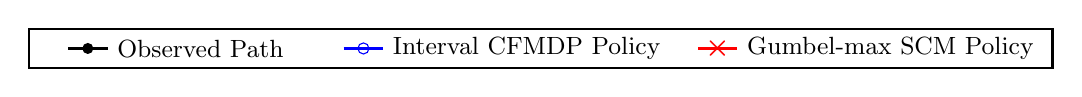
\begin{tikzpicture}[scale=1.0, every node/.style={scale=1.0}]
            \draw[thick, black] (-3, -0.25) rectangle (10, 0.25);
            %
            \draw[black, line width=1pt] (-2.5, 0.0) -- (-2,0.0);
            \fill[black] (-2.25,0.0) circle (2pt); %
            \node[right] at (-2,0.0) {\small Observed Path};
            
            %
            \draw[blue, line width=1pt] (1.0,0.0) -- (1.5,0.0);
            \node[draw=blue, circle, minimum size=4pt, inner sep=0pt] at (1.25,0.0) {}; %
            \node[right] at (1.5,0.0) {\small Interval CFMDP Policy};
            
            %
            \draw[red, line width=1pt] (5.5,0) -- (6,0);
            \node[red] at (5.75,0) {$\boldsymbol{\times}$}; %
            \node[right] at (6,0) {\small Gumbel-max SCM Policy};
        \end{tikzpicture}
    }\\
    %
    \subfigure[\footnotesize Lowest cumulative reward: Interval CFMDP ($312$), Gumbel-max SCM ($312$)]{%
        \resizebox{0.76\columnwidth}{!}{
             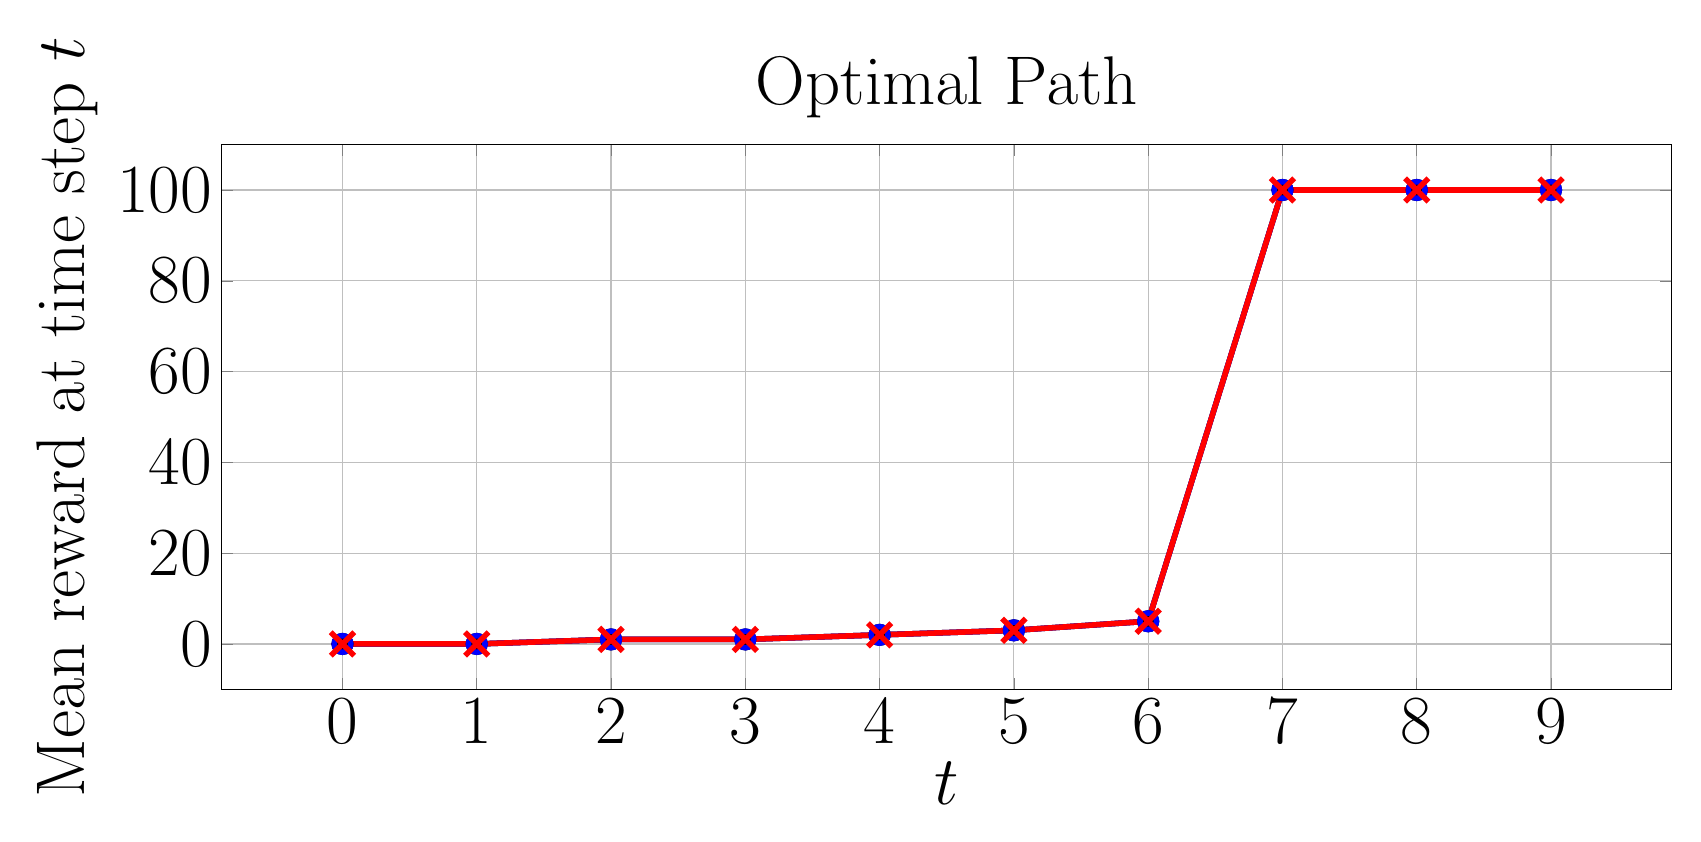
\begin{tikzpicture}
                \begin{axis}[
                    xlabel={$t$},
                    ylabel={Mean reward at time step $t$},
                    title={Optimal Path},
                    grid=both,
                    width=20cm, height=8.5cm,
                    every axis/.style={font=\Huge},
                    %
                ]
                \addplot[
                    color=black, %
                    mark=*, %
                    line width=2pt,
                    mark size=3pt,
                    error bars/.cd,
                    y dir=both, %
                    y explicit, %
                    error bar style={line width=1pt,solid},
                    error mark options={line width=1pt,mark size=4pt,rotate=90}
                ]
                coordinates {
                    (0, 0.0)  +- (0, 0.0)
                    (1, 0.0)  +- (0, 0.0) 
                    (2, 1.0)  +- (0, 0.0) 
                    (3, 1.0)  +- (0, 0.0)
                    (4, 2.0)  +- (0, 0.0)
                    (5, 3.0) +- (0, 0.0)
                    (6, 5.0) +- (0, 0.0)
                    (7, 100.0) +- (0, 0.0)
                    (8, 100.0) +- (0, 0.0)
                    (9, 100.0) +- (0, 0.0)
                };
                %
                \addplot[
                    color=blue, %
                    mark=o, %
                    line width=2pt,
                    mark size=3pt,
                    error bars/.cd,
                    y dir=both, %
                    y explicit, %
                    error bar style={line width=1pt,solid},
                    error mark options={line width=1pt,mark size=4pt,rotate=90}
                ]
                 coordinates {
                    (0, 0.0)  +- (0, 0.0)
                    (1, 0.0)  +- (0, 0.0) 
                    (2, 1.0)  +- (0, 0.0) 
                    (3, 1.0)  +- (0, 0.0)
                    (4, 2.0)  +- (0, 0.0)
                    (5, 3.0) +- (0, 0.0)
                    (6, 5.0) +- (0, 0.0)
                    (7, 100.0) +- (0, 0.0)
                    (8, 100.0) +- (0, 0.0)
                    (9, 100.0) +- (0, 0.0)
                };
                %
                \addplot[
                    color=red, %
                    mark=x, %
                    line width=2pt,
                    mark size=6pt,
                    error bars/.cd,
                    y dir=both, %
                    y explicit, %
                    error bar style={line width=1pt,solid},
                    error mark options={line width=1pt,mark size=4pt,rotate=90}
                ]
                coordinates {
                    (0, 0.0)  +- (0, 0.0)
                    (1, 0.0)  +- (0, 0.0) 
                    (2, 1.0)  +- (0, 0.0) 
                    (3, 1.0)  +- (0, 0.0)
                    (4, 2.0)  +- (0, 0.0)
                    (5, 3.0) +- (0, 0.0)
                    (6, 5.0) +- (0, 0.0)
                    (7, 100.0) +- (0, 0.0)
                    (8, 100.0) +- (0, 0.0)
                    (9, 100.0) +- (0, 0.0)
                };
                \end{axis}
            \end{tikzpicture}
         }
    }
    \hspace{1cm}
    \subfigure[\footnotesize Lowest cumulative reward: Interval CFMDP ($19$), Gumbel-max SCM ($-88$)]{%
         \resizebox{0.76\columnwidth}{!}{
            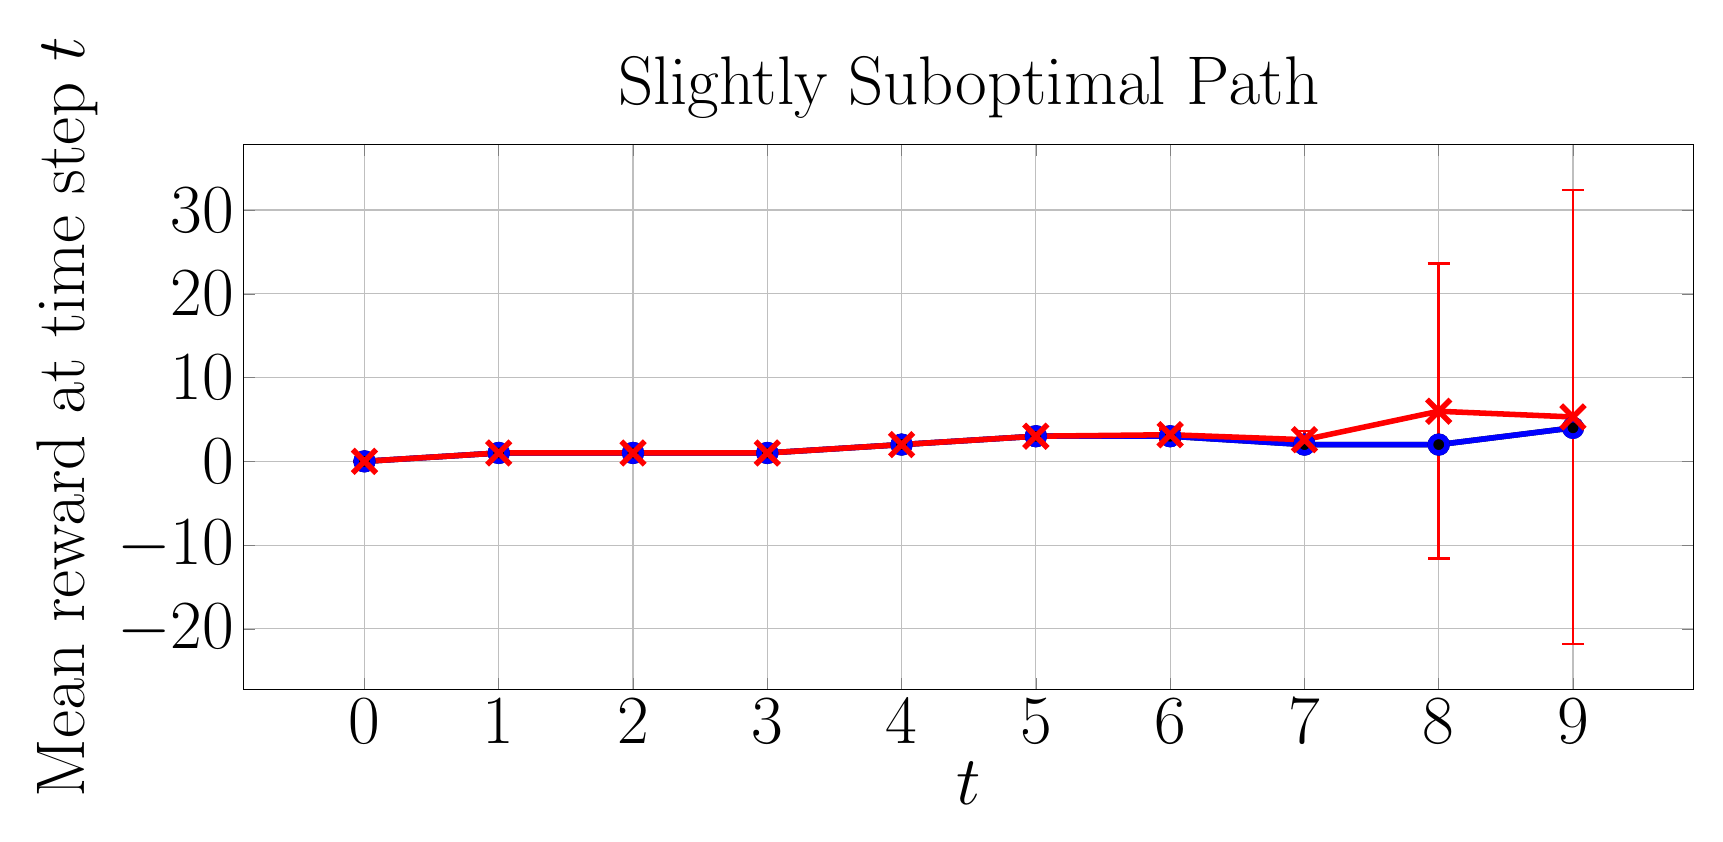
\begin{tikzpicture}
                \begin{axis}[
                    xlabel={$t$},
                    ylabel={Mean reward at time step $t$},
                    title={Slightly Suboptimal Path},
                    grid=both,
                    width=20cm, height=8.5cm,
                    every axis/.style={font=\Huge},
                    %
                ]
                \addplot[
                    color=black, %
                    mark=*, %
                    line width=2pt,
                    mark size=3pt,
                    error bars/.cd,
                    y dir=both, %
                    y explicit, %
                    error bar style={line width=1pt,solid},
                    error mark options={line width=1pt,mark size=4pt,rotate=90}
                ]
              coordinates {
                    (0, 0.0)  +- (0, 0.0)
                    (1, 1.0)  +- (0, 0.0) 
                    (2, 1.0)  +- (0, 0.0) 
                    (3, 1.0)  +- (0, 0.0)
                    (4, 2.0)  +- (0, 0.0)
                    (5, 3.0) +- (0, 0.0)
                    (6, 3.0) +- (0, 0.0)
                    (7, 2.0) +- (0, 0.0)
                    (8, 2.0) +- (0, 0.0)
                    (9, 4.0) +- (0, 0.0)
                };
                %
                \addplot[
                    color=blue, %
                    mark=o, %
                    line width=2pt,
                    mark size=3pt,
                    error bars/.cd,
                    y dir=both, %
                    y explicit, %
                    error bar style={line width=1pt,solid},
                    error mark options={line width=1pt,mark size=4pt,rotate=90}
                ]
              coordinates {
                    (0, 0.0)  +- (0, 0.0)
                    (1, 1.0)  +- (0, 0.0) 
                    (2, 1.0)  +- (0, 0.0) 
                    (3, 1.0)  +- (0, 0.0)
                    (4, 2.0)  +- (0, 0.0)
                    (5, 3.0) +- (0, 0.0)
                    (6, 3.0) +- (0, 0.0)
                    (7, 2.0) +- (0, 0.0)
                    (8, 2.0) +- (0, 0.0)
                    (9, 4.0) +- (0, 0.0)
                };
                %
                \addplot[
                    color=red, %
                    mark=x, %
                    line width=2pt,
                    mark size=6pt,
                    error bars/.cd,
                    y dir=both, %
                    y explicit, %
                    error bar style={line width=1pt,solid},
                    error mark options={line width=1pt,mark size=4pt,rotate=90}
                ]
                coordinates {
                    (0, 0.0)  +- (0, 0.0)
                    (1, 1.0)  +- (0, 0.0) 
                    (2, 1.0)  +- (0, 0.0) 
                    (3, 1.0)  +- (0, 0.0)
                    (4, 2.0)  += (0, 0.0)
                    (5, 3.0)  += (0, 0.0)
                    (6, 3.17847) += (0, 0.62606746) -= (0, 0.62606746)
                    (7, 2.5832885) += (0, 1.04598233) -= (0, 1.04598233)
                    (8, 5.978909) += (0, 17.60137623) -= (0, 17.60137623)
                    (9, 5.297059) += (0, 27.09227512) -= (0, 27.09227512)
                };
                \end{axis}
            \end{tikzpicture}
         }
    }\\[-1.5pt]
    \subfigure[\footnotesize Lowest cumulative reward: Interval CFMDP ($14$), Gumbel-max SCM ($-598$)]{%
         \resizebox{0.76\columnwidth}{!}{
             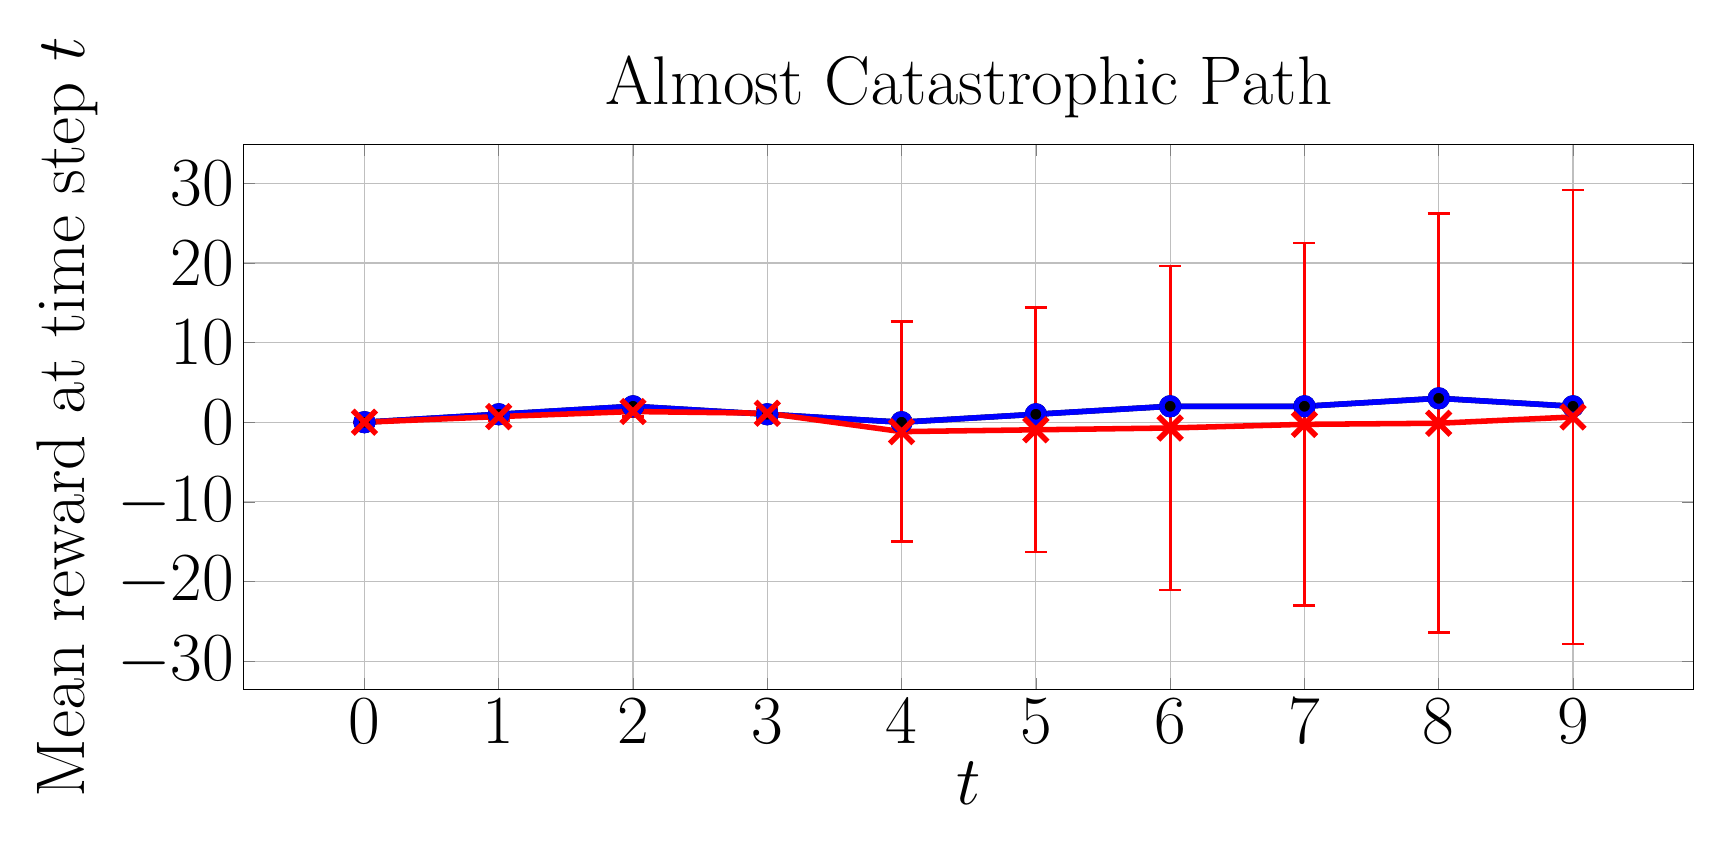
\begin{tikzpicture}
                \begin{axis}[
                    xlabel={$t$},
                    ylabel={Mean reward at time step $t$},
                    title={Almost Catastrophic Path},
                    grid=both,
                    width=20cm, height=8.5cm,
                    every axis/.style={font=\Huge},
                    %
                ]
                \addplot[
                    color=black, %
                    mark=*, %
                    line width=2pt,
                    mark size=3pt,
                    error bars/.cd,
                    y dir=both, %
                    y explicit, %
                    error bar style={line width=1pt,solid},
                    error mark options={line width=1pt,mark size=4pt,rotate=90}
                ]
                coordinates {
                    (0, 0.0)  +- (0, 0.0)
                    (1, 1.0)  +- (0, 0.0) 
                    (2, 2.0)  +- (0, 0.0) 
                    (3, 1.0)  +- (0, 0.0)
                    (4, 0.0)  +- (0, 0.0)
                    (5, 1.0) +- (0, 0.0)
                    (6, 2.0) +- (0, 0.0)
                    (7, 2.0) +- (0, 0.0)
                    (8, 3.0) +- (0, 0.0)
                    (9, 2.0) +- (0, 0.0)
                };
                %
                \addplot[
                    color=blue, %
                    mark=o, %
                    line width=2pt,
                    mark size=3pt,
                    error bars/.cd,
                    y dir=both, %
                    y explicit, %
                    error bar style={line width=1pt,solid},
                    error mark options={line width=1pt,mark size=4pt,rotate=90}
                ]
                coordinates {
                    (0, 0.0)  +- (0, 0.0)
                    (1, 1.0)  +- (0, 0.0) 
                    (2, 2.0)  +- (0, 0.0) 
                    (3, 1.0)  +- (0, 0.0)
                    (4, 0.0)  +- (0, 0.0)
                    (5, 1.0) +- (0, 0.0)
                    (6, 2.0) +- (0, 0.0)
                    (7, 2.0) +- (0, 0.0)
                    (8, 3.0) +- (0, 0.0)
                    (9, 2.0) +- (0, 0.0)
                };
                %
                \addplot[
                    color=red, %
                    mark=x, %
                    line width=2pt,
                    mark size=6pt,
                    error bars/.cd,
                    y dir=both, %
                    y explicit, %
                    error bar style={line width=1pt,solid},
                    error mark options={line width=1pt,mark size=4pt,rotate=90}
                ]
                coordinates {
                    (0, 0.0)  +- (0, 0.0)
                    (1, 0.7065655)  +- (0, 0.4553358) 
                    (2, 1.341673)  +- (0, 0.67091621) 
                    (3, 1.122926)  +- (0, 0.61281824)
                    (4, -1.1821935)  +- (0, 13.82444042)
                    (5, -0.952399)  +- (0, 15.35195457)
                    (6, -0.72672) +- (0, 20.33508414)
                    (7, -0.268983) +- (0, 22.77861454)
                    (8, -0.1310835) +- (0, 26.31013314)
                    (9, 0.65806) +- (0, 28.50670214)
                };
                %
            %
            %
            %
            %
            %
            %
            %
            %
            %
            %
            %
            %
            %
            %
            %
            %
            %
            %
                \end{axis}
            \end{tikzpicture}
         }
    }
    \hspace{1cm}
    \subfigure[\footnotesize Lowest cumulative reward: Interval CFMDP ($-698$), Gumbel-max SCM ($-698$)]{%
         \resizebox{0.76\columnwidth}{!}{
            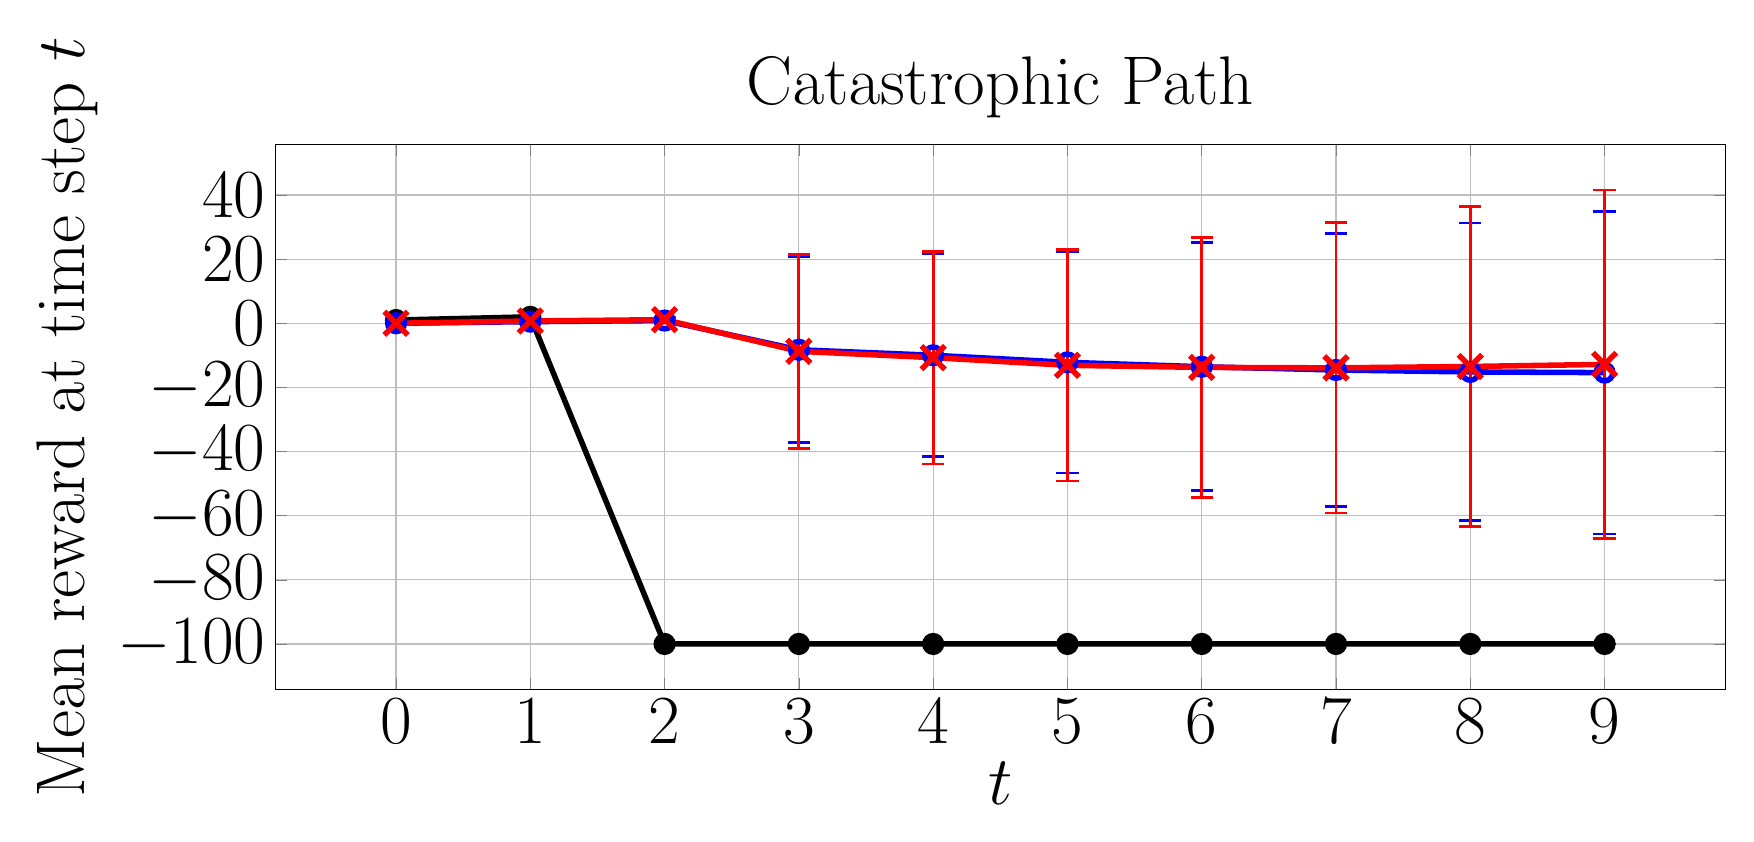
\begin{tikzpicture}
                \begin{axis}[
                    xlabel={$t$},
                    ylabel={Mean reward at time step $t$},
                    title={Catastrophic Path},
                    grid=both,
                    width=20cm, height=8.5cm,
                    every axis/.style={font=\Huge},
                    %
                ]
                \addplot[
                    color=black, %
                    mark=*, %
                    line width=2pt,
                    mark size=3pt,
                    error bars/.cd,
                    y dir=both, %
                    y explicit, %
                    error bar style={line width=1pt,solid},
                    error mark options={line width=1pt,mark size=4pt,rotate=90}
                ]
                coordinates {
                    (0, 1.0)  +- (0, 0.0)
                    (1, 2.0)  +- (0, 0.0) 
                    (2, -100.0)  +- (0, 0.0) 
                    (3, -100.0)  +- (0, 0.0)
                    (4, -100.0)  +- (0, 0.0)
                    (5, -100.0) +- (0, 0.0)
                    (6, -100.0) +- (0, 0.0)
                    (7, -100.0) +- (0, 0.0)
                    (8, -100.0) +- (0, 0.0)
                    (9, -100.0) +- (0, 0.0)
                };
                %
                \addplot[
                    color=blue, %
                    mark=o, %
                    line width=2pt,
                    mark size=3pt,
                    error bars/.cd,
                    y dir=both, %
                    y explicit, %
                    error bar style={line width=1pt,solid},
                    error mark options={line width=1pt,mark size=4pt,rotate=90}
                ]
                coordinates {
                    (0, 0.0)  +- (0, 0.0)
                    (1, 0.504814)  +- (0, 0.49997682) 
                    (2, 0.8439835)  +- (0, 0.76831917) 
                    (3, -8.2709165)  +- (0, 28.93656754)
                    (4, -9.981082)  +- (0, 31.66825363)
                    (5, -12.1776325) +- (0, 34.53463233)
                    (6, -13.556076) +- (0, 38.62845372)
                    (7, -14.574418) +- (0, 42.49603359)
                    (8, -15.1757075) +- (0, 46.41913968)
                    (9, -15.3900395) +- (0, 50.33563368)
                };
                %
                \addplot[
                    color=red, %
                    mark=x, %
                    line width=2pt,
                    mark size=6pt,
                    error bars/.cd,
                    y dir=both, %
                    y explicit, %
                    error bar style={line width=1pt,solid},
                    error mark options={line width=1pt,mark size=4pt,rotate=90}
                ]
                coordinates {
                    (0, 0.0)  +- (0, 0.0)
                    (1, 0.701873)  +- (0, 0.45743556) 
                    (2, 1.1227805)  +- (0, 0.73433129) 
                    (3, -8.7503255)  +- (0, 30.30257976)
                    (4, -10.722092)  +- (0, 33.17618589)
                    (5, -13.10721)  +- (0, 36.0648089)
                    (6, -13.7631645) +- (0, 40.56553451)
                    (7, -13.909043) +- (0, 45.23829402)
                    (8, -13.472517) +- (0, 49.96270296)
                    (9, -12.8278835) +- (0, 54.38618735)
                };
                %
            %
            %
            %
            %
            %
            %
            %
            %
            %
            %
            %
            %
            %
            %
            %
            %
            %
            %
                \end{axis}
            \end{tikzpicture}
         }
    }
    \caption{Average instant reward of CF paths induced by policies on GridWorld $p=0.4$.}
    \label{fig: reward p=0.4}
\end{figure*}

\subsection{Experimental Setup}
To compare policy performance, we measure the average rewards of counterfactual paths induced by our policy and the Gumbel-max policy by uniformly sampling $200$ counterfactual MDPs from the ICFMDP and generating $10,000$ counterfactual paths over each sampled CFMDP. \jl{Since the interval CFMDP depends on the observed path, we select $4$  paths of varying optimality to evaluate how the observed path impacts the performance of both policies: an optimal path, a slightly suboptimal path that could reach the optimal reward with a few changes, a catastrophic path that enters a catastrophic, terminal state with low reward, and an almost catastrophic path that was close to entering a catastrophic state.} When measuring the average probability bound widths and execution time needed to generate the ICFMDPs, we averaged over $20$ randomly generated observed paths
\footnote{Further training details are provided in Appendix \ref{app: training details}, and the code is provided at \href{https://github.com/ddv-lab/robust-cf-inference-in-MDPs}{https://github.com/ddv-lab/robust-cf-inference-in-MDPs}
%
%
.}.

\subsection{GridWorld}
\jl{The GridWorld MDP is a $4 \times 4$ grid where an agent must navigate from the top-left corner to the goal state in the bottom-right corner, avoiding a dangerous terminal state in the centre. At each time step, the agent can move up, down, left, or right, but there is a small probability (controlled by hyper-parameter $p$) of moving in an unintended direction. As the agent nears the goal, the reward for each state increases, culminating in a reward of $+100$ for reaching the goal. Entering the dangerous state results in a penalty of $-100$. We use two versions of GridWorld: a less stochastic version with $p=0.9$ (i.e., $90$\% chance of moving in the chosen direction) and a more stochastic version with $p=0.4$.}

\paragraph{GridWorld ($p=0.9$)}
When $p=0.9$, the counterfactual probability bounds are typically narrow (see Table \ref{tab:nonzero_probs} for average measurements). Consequently, as shown in Figure \ref{fig: reward p=0.9}, both policies are nearly identical and perform similarly well across the optimal, slightly suboptimal, and catastrophic paths.
%
However, for the almost catastrophic path, the interval CFMDP path is more conservative and follows the observed path more closely (as this is where the probability bounds are narrowest), which typically requires one additional step to reach the goal state than the Gumbel-max SCM policy.
%

\paragraph{GridWorld ($p=0.4$)}
\jl{When $p=0.4$, the GridWorld environment becomes more uncertain, increasing the risk of entering the dangerous state even if correct actions are chosen. Thus, as shown in Figure \ref{fig: reward p=0.4}, the interval CFMDP policy adopts a more conservative approach, avoiding deviation from the observed policy if it cannot guarantee higher counterfactual rewards (see the slightly suboptimal and almost catastrophic paths), whereas the Gumbel-max SCM is inconsistent: it can yield higher rewards, but also much lower rewards, reflected in the wide error bars.} For the catastrophic path, both policies must deviate from the observed path to achieve a higher reward and, in this case, perform similarly.
%
%
%
%
\subsection{Sepsis}
The Sepsis MDP \citep{oberst2019counterfactual} simulates trajectories of Sepsis patients. Each state consists of four vital signs (heart rate, blood pressure, oxygen concentration, and glucose levels), categorised as low, normal, or high.
and three treatments that can be toggled on/off at each time step (8 actions in total). Unlike \citet{oberst2019counterfactual}, we scale rewards based on the number of out-of-range vital signs, between $-1000$ (patient dies) and $1000$ (patient discharged). \jl{Like the GridWorld $p=0.4$ experiment, the Sepsis MDP is highly uncertain, as many states are equally likely to lead to optimal and poor outcomes. Thus, as shown in Figure \ref{fig: reward sepsis}, both policies follow the observed optimal and almost catastrophic paths to guarantee rewards are no worse than the observation.} However, improving the catastrophic path requires deviating from the observation. Here, the Gumbel-max SCM policy, on average, performs better than the interval CFMDP policy. But, since both policies have lower bounds clipped at $-1000$, neither policy reliably improves over the observation. In contrast, for the slightly suboptimal path, the interval CFMDP policy performs significantly better, shown by its higher lower bounds. 
Moreover, in these two cases, the worst-case counterfactual path generated by the interval CFMDP policy is better than that of the Gumbel-max SCM policy,
indicating its greater robustness.
%
\begin{figure*}
    \centering
     \resizebox{0.6\textwidth}{!}{
        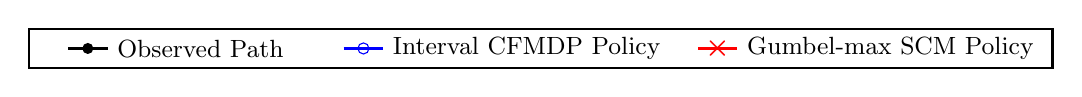
\begin{tikzpicture}[scale=1.0, every node/.style={scale=1.0}]
            \draw[thick, black] (-3, -0.25) rectangle (10, 0.25);
            %
            \draw[black, line width=1pt] (-2.5, 0.0) -- (-2,0.0);
            \fill[black] (-2.25,0.0) circle (2pt); %
            \node[right] at (-2,0.0) {\small Observed Path};
            
            %
            \draw[blue, line width=1pt] (1.0,0.0) -- (1.5,0.0);
            \node[draw=blue, circle, minimum size=4pt, inner sep=0pt] at (1.25,0.0) {}; %
            \node[right] at (1.5,0.0) {\small Interval CFMDP Policy};
            
            %
            \draw[red, line width=1pt] (5.5,0) -- (6,0);
            \node[red] at (5.75,0) {$\boldsymbol{\times}$}; %
            \node[right] at (6,0) {\small Gumbel-max SCM Policy};
        \end{tikzpicture}
    }\\
    \subfigure[\footnotesize Lowest cumulative reward: Interval CFMDP ($8000$), Gumbel-max SCM ($8000$)]{%
         \resizebox{0.76\columnwidth}{!}{
             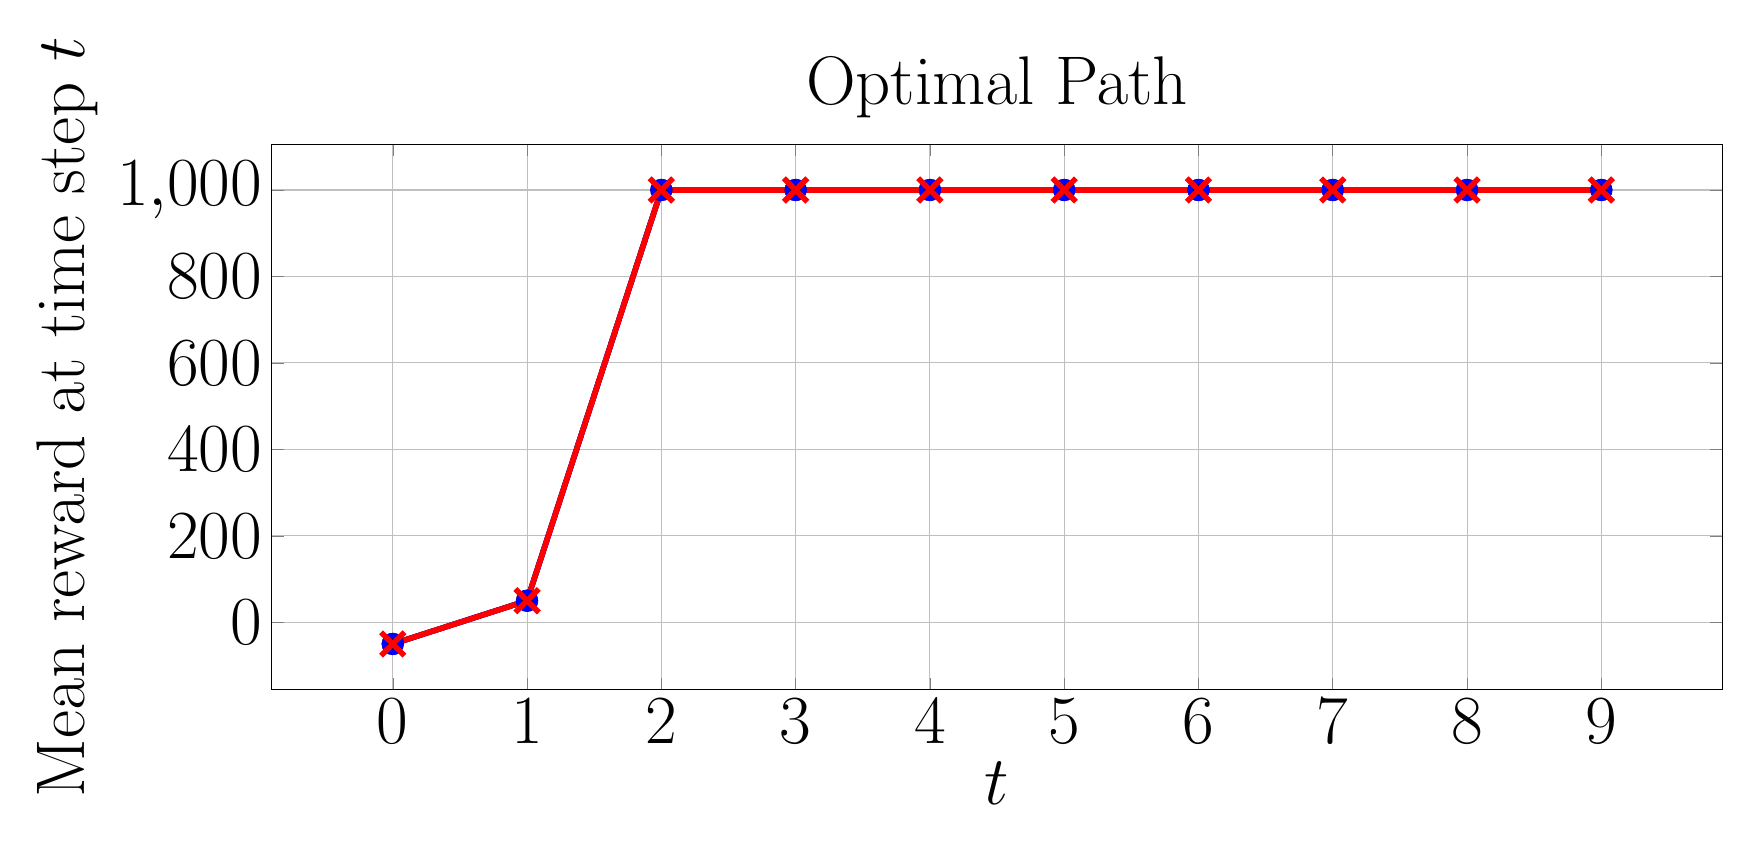
\begin{tikzpicture}
                \begin{axis}[
                    xlabel={$t$},
                    ylabel={Mean reward at time step $t$},
                    title={Optimal Path},
                    grid=both,
                    width=20cm, height=8.5cm,
                    every axis/.style={font=\Huge},
                    %
                ]
                \addplot[
                    color=black, %
                    mark=*, %
                    line width=2pt,
                    mark size=3pt,
                ]
                coordinates {
                    (0, -50.0)
                    (1, 50.0)
                    (2, 1000.0)
                    (3, 1000.0)
                    (4, 1000.0)
                    (5, 1000.0)
                    (6, 1000.0)
                    (7, 1000.0)
                    (8, 1000.0)
                    (9, 1000.0)
                };
                %
                \addplot[
                    color=blue, %
                    mark=o, %
                    line width=2pt,
                    mark size=3pt,
                    error bars/.cd,
                    y dir=both, %
                    y explicit, %
                    error bar style={line width=1pt,solid},
                    error mark options={line width=1pt,mark size=4pt,rotate=90}
                ]
                coordinates {
                    (0, -50.0)  +- (0, 0.0)
                    (1, 50.0)  +- (0, 0.0) 
                    (2, 1000.0)  +- (0, 0.0) 
                    (3, 1000.0)  +- (0, 0.0)
                    (4, 1000.0)  +- (0, 0.0)
                    (5, 1000.0) +- (0, 0.0)
                    (6, 1000.0) +- (0, 0.0)
                    (7, 1000.0) +- (0, 0.0)
                    (8, 1000.0) +- (0, 0.0)
                    (9, 1000.0) +- (0, 0.0)
                };
                %
                \addplot[
                    color=red, %
                    mark=x, %
                    line width=2pt,
                    mark size=6pt,
                    error bars/.cd,
                    y dir=both, %
                    y explicit, %
                    error bar style={line width=1pt,solid},
                    error mark options={line width=1pt,mark size=4pt,rotate=90}
                ]
                coordinates {
                    (0, -50.0)  +- (0, 0.0)
                    (1, 50.0)  +- (0, 0.0) 
                    (2, 1000.0)  +- (0, 0.0) 
                    (3, 1000.0)  +- (0, 0.0)
                    (4, 1000.0)  +- (0, 0.0)
                    (5, 1000.0) +- (0, 0.0)
                    (6, 1000.0) +- (0, 0.0)
                    (7, 1000.0) +- (0, 0.0)
                    (8, 1000.0) +- (0, 0.0)
                    (9, 1000.0) +- (0, 0.0)
                };
                %
                \end{axis}
            \end{tikzpicture}
         }
    }
    \hspace{1cm}
    \subfigure[\footnotesize Lowest cumulative reward: Interval CFMDP ($-5980$), Gumbel-max SCM ($-8000$)]{%
         \resizebox{0.76\columnwidth}{!}{
            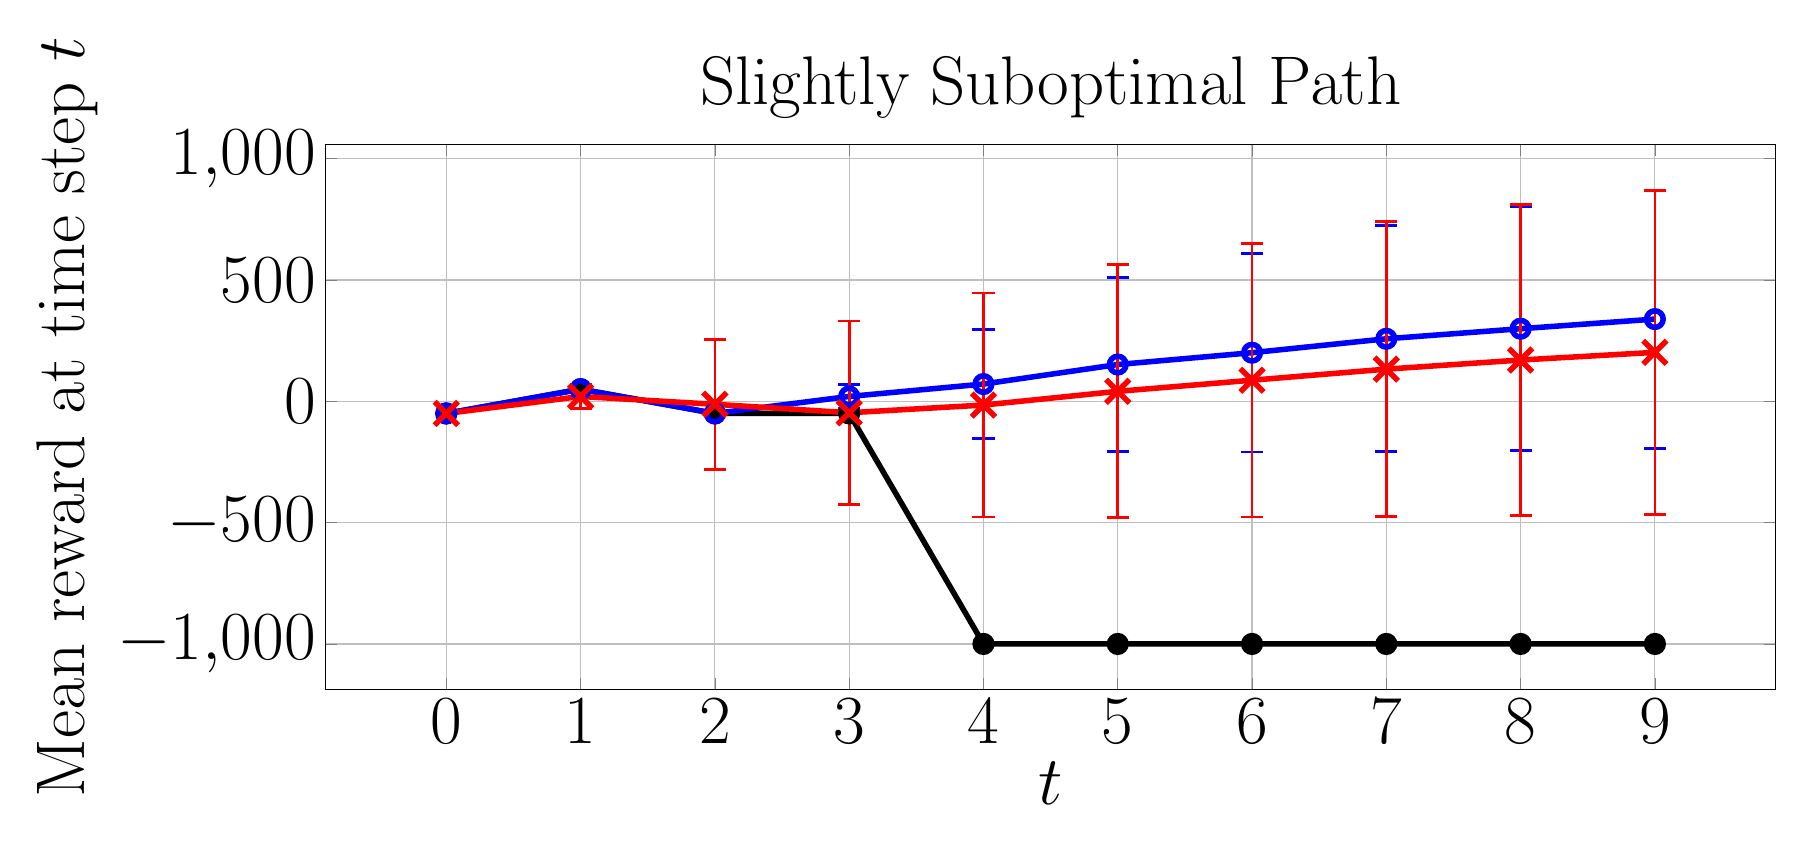
\begin{tikzpicture}
                \begin{axis}[
                    xlabel={$t$},
                    ylabel={Mean reward at time step $t$},
                    title={Slightly Suboptimal Path},
                    grid=both,
                    width=20cm, height=8.5cm,
                    every axis/.style={font=\Huge},
                    %
                ]
               \addplot[
                    color=black, %
                    mark=*, %
                    line width=2pt,
                    mark size=3pt,
                ]
                coordinates {
                    (0, -50.0)
                    (1, 50.0)
                    (2, -50.0)
                    (3, -50.0)
                    (4, -1000.0)
                    (5, -1000.0)
                    (6, -1000.0)
                    (7, -1000.0)
                    (8, -1000.0)
                    (9, -1000.0)
                };
                %
                \addplot[
                    color=blue, %
                    mark=o, %
                    line width=2pt,
                    mark size=3pt,
                    error bars/.cd,
                    y dir=both, %
                    y explicit, %
                    error bar style={line width=1pt,solid},
                    error mark options={line width=1pt,mark size=4pt,rotate=90}
                ]
                coordinates {
                    (0, -50.0)  +- (0, 0.0)
                    (1, 50.0)  +- (0, 0.0) 
                    (2, -50.0)  +- (0, 0.0) 
                    (3, 20.0631)  +- (0, 49.97539413)
                    (4, 71.206585)  +- (0, 226.02033693)
                    (5, 151.60797) +- (0, 359.23292559)
                    (6, 200.40593) +- (0, 408.86185176)
                    (7, 257.77948) +- (0, 466.10372804)
                    (8, 299.237465) +- (0, 501.82579506)
                    (9, 338.9129) +- (0, 532.06124996)
                };
                %
                \addplot[
                    color=red, %
                    mark=x, %
                    line width=2pt,
                    mark size=6pt,
                    error bars/.cd,
                    y dir=both, %
                    y explicit, %
                    error bar style={line width=1pt,solid},
                    error mark options={line width=1pt,mark size=4pt,rotate=90}
                ]
                coordinates {
                    (0, -50.0)  +- (0, 0.0)
                    (1, 20.00736)  +- (0, 49.99786741) 
                    (2, -12.282865)  +- (0, 267.598755) 
                    (3, -47.125995)  +- (0, 378.41755832)
                    (4, -15.381965)  +- (0, 461.77616558)
                    (5, 41.15459) +- (0, 521.53189262)
                    (6, 87.01595) +- (0, 564.22243126 )
                    (7, 132.62376) +- (0, 607.31338037)
                    (8, 170.168145) +- (0, 641.48013693)
                    (9, 201.813135) +- (0, 667.29441777)
                };
                %
                %
                %
                %
                %
                %
                %
                %
                %
                %
                %
                %
                %
                %
                %
                %
                %
                %
                %
                \end{axis}
            \end{tikzpicture}
         }
    }\\[-1.5pt]
    \subfigure[\footnotesize Lowest cumulative reward: Interval CFMDP ($100$), Gumbel-max SCM ($100$)]{%
         \resizebox{0.76\columnwidth}{!}{
             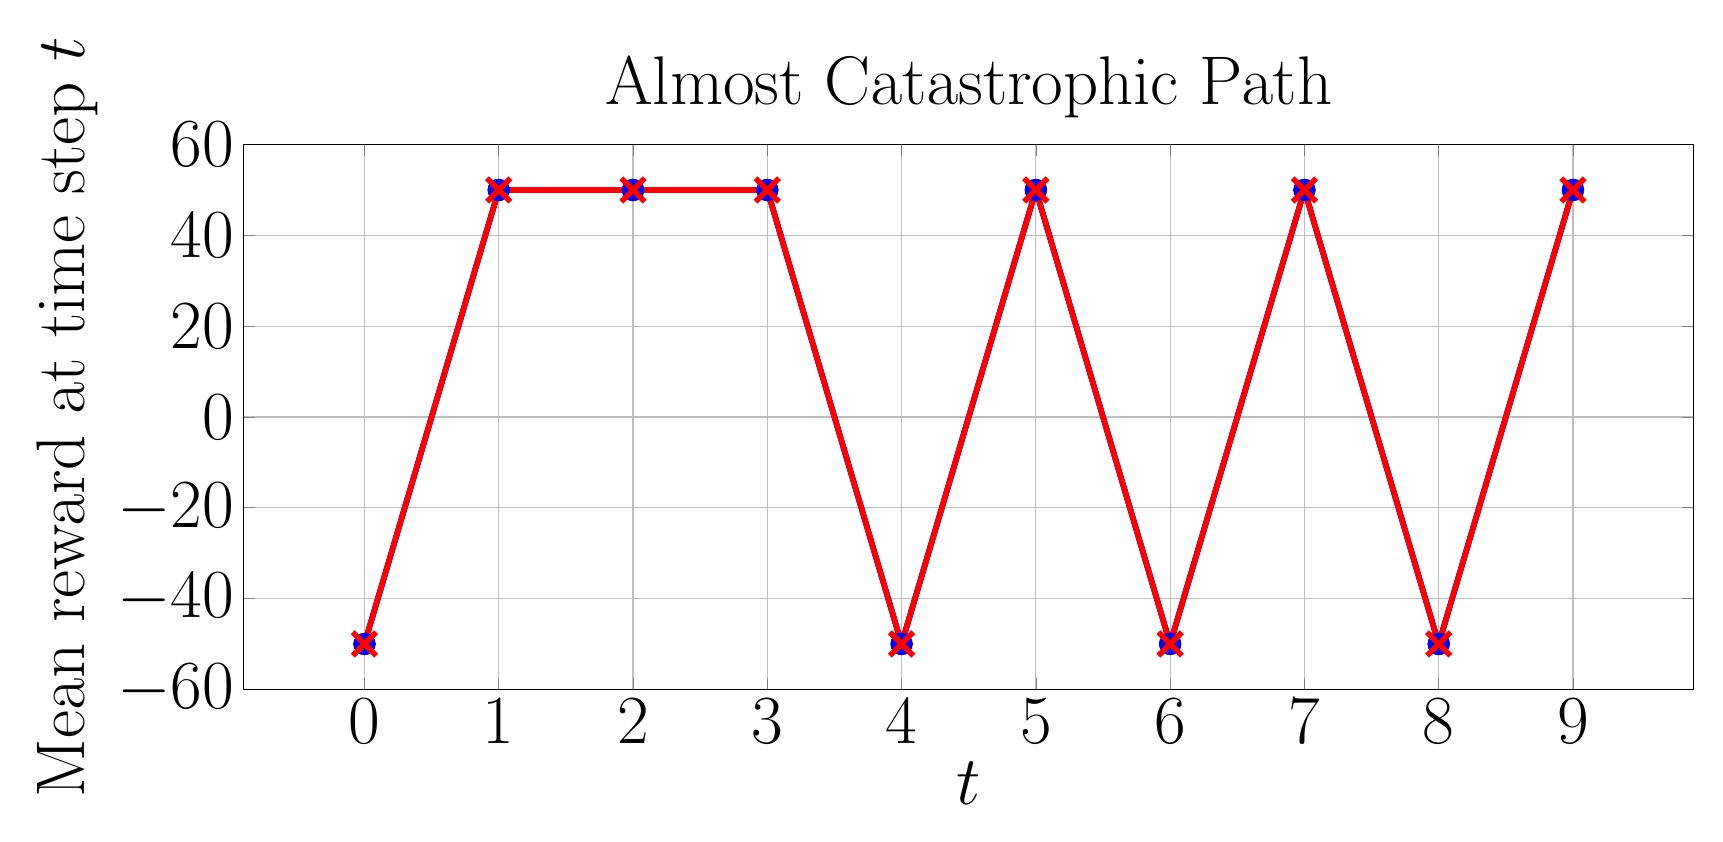
\begin{tikzpicture}
                \begin{axis}[
                    xlabel={$t$},
                    ylabel={Mean reward at time step $t$},
                    title={Almost Catastrophic Path},
                    grid=both,
                    every axis/.style={font=\Huge},
                    width=20cm, height=8.5cm,
                    %
                ]
               \addplot[
                    color=black, %
                    mark=*, %
                    line width=2pt,
                    mark size=3pt,
                ]
                coordinates {
                    (0, -50.0)
                    (1, 50.0)
                    (2, 50.0)
                    (3, 50.0)
                    (4, -50.0)
                    (5, 50.0)
                    (6, -50.0)
                    (7, 50.0)
                    (8, -50.0)
                    (9, 50.0)
                };
                %
                %
                \addplot[
                    color=blue, %
                    mark=o, %
                    line width=2pt,
                    mark size=3pt,
                    error bars/.cd,
                    y dir=both, %
                    y explicit, %
                    error bar style={line width=1pt,solid},
                    error mark options={line width=1pt,mark size=4pt,rotate=90}
                ]
                coordinates {
                    (0, -50.0)  +- (0, 0.0)
                    (1, 50.0)  +- (0, 0.0) 
                    (2, 50.0)  +- (0, 0.0) 
                    (3, 50.0)  +- (0, 0.0)
                    (4, -50.0)  +- (0, 0.0)
                    (5, 50.0) +- (0, 0.0)
                    (6, -50.0) +- (0, 0.0)
                    (7, 50.0) +- (0, 0.0)
                    (8, -50.0) +- (0, 0.0)
                    (9, 50.0) +- (0, 0.0)
                };
                %
                \addplot[
                    color=red, %
                    mark=x, %
                    line width=2pt,
                    mark size=6pt,
                    error bars/.cd,
                    y dir=both, %
                    y explicit, %
                    error bar style={line width=1pt,solid},
                    error mark options={line width=1pt,mark size=4pt,rotate=90}
                ]
                coordinates {
                    (0, -50.0)  +- (0, 0.0)
                    (1, 50.0)  +- (0, 0.0) 
                    (2, 50.0)  +- (0, 0.0) 
                    (3, 50.0)  +- (0, 0.0)
                    (4, -50.0)  +- (0, 0.0)
                    (5, 50.0) +- (0, 0.0)
                    (6, -50.0) +- (0, 0.0)
                    (7, 50.0) +- (0, 0.0)
                    (8, -50.0) +- (0, 0.0)
                    (9, 50.0) +- (0, 0.0)
                };
                %
                %
                %
                %
                %
                %
                %
                %
                %
                %
                %
                %
                %
                %
                %
                %
                %
                %
                %
                \end{axis}
            \end{tikzpicture}
         }
    }
    \hspace{1cm}
    \subfigure[\footnotesize Lowest cumulative reward: Interval CFMDP ($-7150$), Gumbel-max SCM ($-9050$)]{%
         \resizebox{0.76\columnwidth}{!}{
            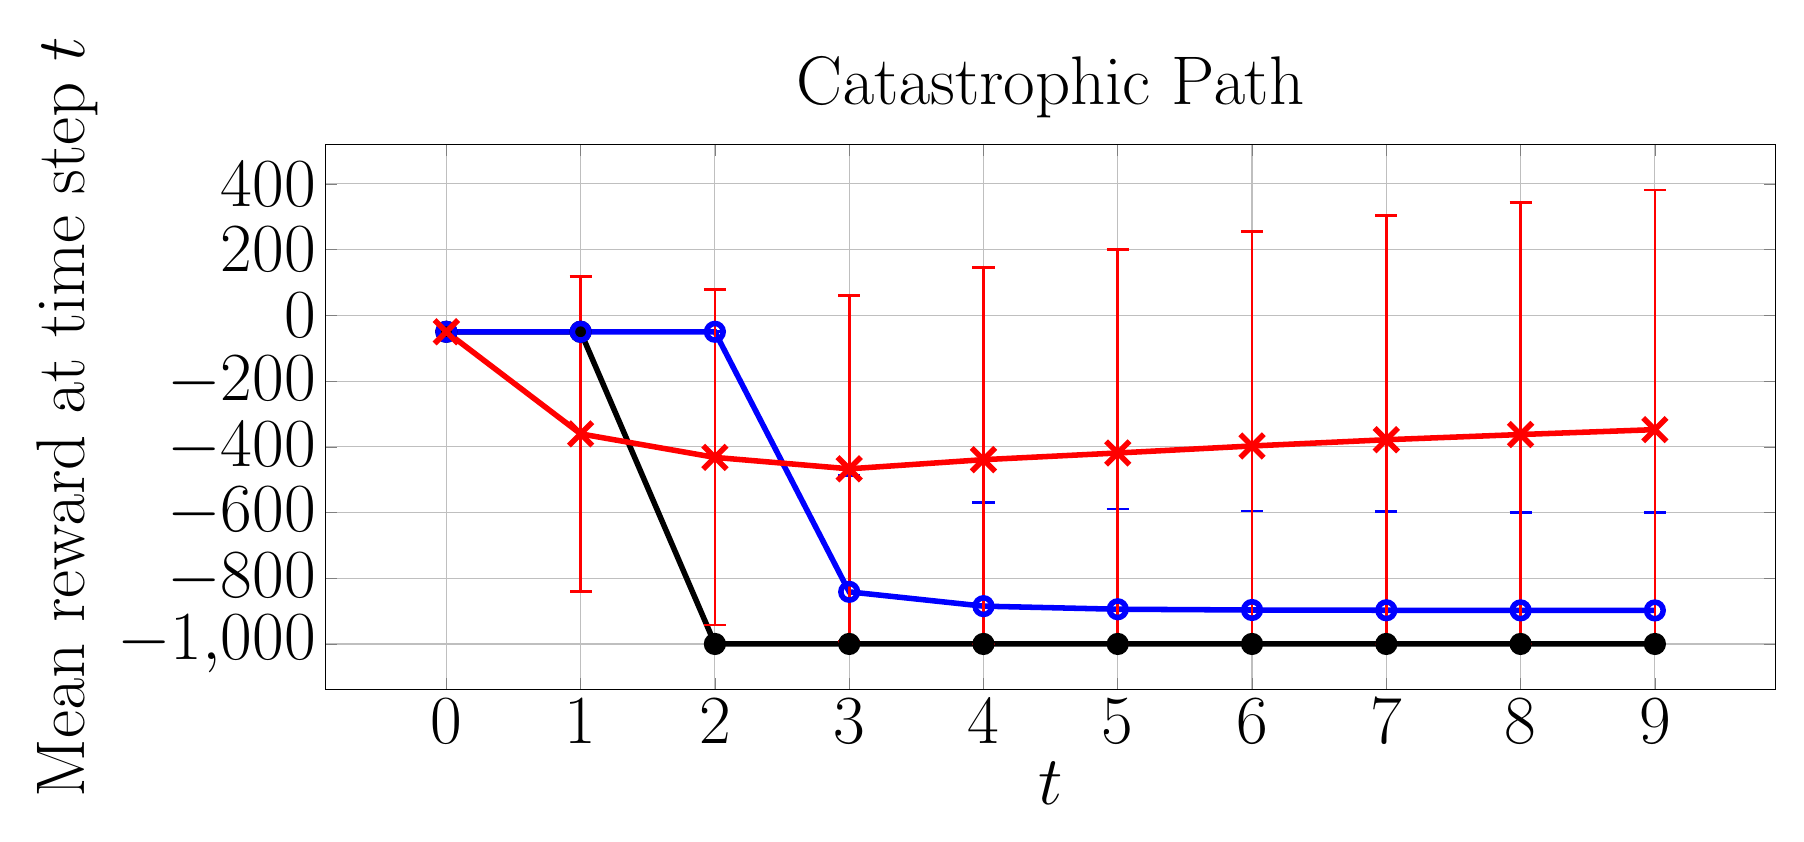
\begin{tikzpicture}
                \begin{axis}[
                    xlabel={$t$},
                    ylabel={Mean reward at time step $t$},
                    title={Catastrophic Path},
                    grid=both,
                    width=20cm, height=8.5cm,
                    every axis/.style={font=\Huge},
                    %
                ]
               \addplot[
                    color=black, %
                    mark=*, %
                    line width=2pt,
                    mark size=3pt,
                ]
                coordinates {
                    (0, -50.0)
                    (1, -50.0)
                    (2, -1000.0)
                    (3, -1000.0)
                    (4, -1000.0)
                    (5, -1000.0)
                    (6, -1000.0)
                    (7, -1000.0)
                    (8, -1000.0)
                    (9, -1000.0)
                };
                %
                %
                \addplot[
                    color=blue, %
                    mark=o, %
                    line width=2pt,
                    mark size=3pt,
                    error bars/.cd,
                    y dir=both, %
                    y explicit, %
                    error bar style={line width=1pt,solid},
                    error mark options={line width=1pt,mark size=4pt,rotate=90}
                ]
                coordinates {
                    (0, -50.0)  +- (0, 0.0)
                    (1, -50.0)  +- (0, 0.0) 
                    (2, -50.0)  +- (0, 0.0) 
                    (3, -841.440725)  += (0, 354.24605512) -= (0, 158.559275)
                    (4, -884.98225)  += (0, 315.37519669) -= (0, 115.01775)
                    (5, -894.330425) += (0, 304.88572805) -= (0, 105.669575)
                    (6, -896.696175) += (0, 301.19954514) -= (0, 103.303825)
                    (7, -897.4635) += (0, 299.61791279) -= (0, 102.5365)
                    (8, -897.77595) += (0, 298.80392585) -= (0, 102.22405)
                    (9, -897.942975) += (0, 298.32920557) -= (0, 102.057025)
                };
                %
                \addplot[
                    color=red, %
                    mark=x, %
                    line width=2pt,
                    mark size=6pt,
                    error bars/.cd,
                    y dir=both, %
                    y explicit, %
                    error bar style={line width=1pt,solid},
                    error mark options={line width=1pt,mark size=4pt,rotate=90}
                ]
            coordinates {
                    (0, -50.0)  +- (0, 0.0)
                    (1, -360.675265)  +- (0, 479.39812699) 
                    (2, -432.27629)  +- (0, 510.38620897) 
                    (3, -467.029545)  += (0, 526.36009628) -= (0, 526.36009628)
                    (4, -439.17429)  += (0, 583.96638919) -= (0, 560.82571)
                    (5, -418.82704) += (0, 618.43027478) -= (0, 581.17296)
                    (6, -397.464895) += (0, 652.67322574) -= (0, 602.535105)
                    (7, -378.49052) += (0, 682.85407033) -= (0, 621.50948)
                    (8, -362.654195) += (0, 707.01412023) -= (0, 637.345805)
                    (9, -347.737935) += (0, 729.29076479) -= (0, 652.262065)
                };
                %
                %
                %
                %
                %
                %
                %
                %
                %
                %
                %
                %
                %
                %
                %
                %
                %
                %
                %
                \end{axis}
            \end{tikzpicture}
         }
    }
    \caption{Average instant reward of CF paths induced by policies on Sepsis.}
    \label{fig: reward sepsis}
\end{figure*}

%
%
%
\subsection{Interval CFMDP Bounds}
%
%
Table \ref{tab:nonzero_probs} presents the mean counterfactual probability bound widths (excluding transitions where the upper bound is $0$) for each MDP, averaged over 20 observed paths. We compare the bounds under counterfactual stability (CS) and monotonicity (M) assumptions, CS alone, and no assumptions. This shows that the assumptions marginally reduce the bound widths, indicating the assumptions tighten the bounds without excluding too many causal models, as intended.
\renewcommand{\arraystretch}{1}

\begin{table}
\centering
\caption{Mean width of counterfactual probability bounds}
\resizebox{0.8\columnwidth}{!}{%
\begin{tabular}{|c|c|c|c|}
\hline
\multirow{2}{*}{\textbf{Environment}} & \multicolumn{3}{c|}{\textbf{Assumptions}} \\ \cline{2-4}
 & \textbf{CS + M} & \textbf{CS} & \textbf{None\tablefootnote{\jl{Equivalent to \citet{li2024probabilities}'s bounds (see Section \ref{sec: equivalence with Li}).}}} \\ \hline
\textbf{GridWorld} ($p=0.9$) & 0.0817 & 0.0977 & 0.100 \\ \hline
\textbf{GridWorld} ($p=0.4$) & 0.552  & 0.638  & 0.646 \\ \hline
\textbf{Sepsis} & 0.138 & 0.140 & 0.140 \\ \hline
\end{tabular}
}
\label{tab:nonzero_probs}
\end{table}


\subsection{Execution Times}
Table \ref{tab: times} compares the average time needed to generate the interval CFMDP vs.\ the Gumbel-max SCM CFMDP for 20 observations.
The GridWorld algorithms were run single-threaded, while the Sepsis experiments were run in parallel.
Generating the interval CFMDP is significantly faster as it uses exact analytical bounds, whereas the Gumbel-max CFMDP requires sampling from the Gumbel distribution to estimate counterfactual transition probabilities. \jl{Since constructing the counterfactual MDP models is the main bottleneck in both approaches, ours is more efficient overall and suitable for larger MDPs.}
\begin{table}
\centering
\caption{Mean execution time to generate CFMDPs}
\resizebox{0.99\columnwidth}{!}{%
\begin{tabular}{|c|c|c|}
\hline
\multirow{2}{*}{\textbf{Environment}} & \multicolumn{2}{c|}{\textbf{Mean Execution Time (s)}} \\ \cline{2-3} 
                                      & \textbf{Interval CFMDP} & \textbf{Gumbel-max CFMDP} \\ \hline
\textbf{GridWorld ($p=0.9$) }                  & 0.261                   & 56.1                      \\ \hline
\textbf{GridWorld ($p=0.4$)  }                 & 0.336                   & 54.5                      \\ \hline
\textbf{Sepsis}                                 & 688                     & 2940                      \\ \hline
\end{tabular}%
}
\label{tab: times}
\end{table}

\section{Results}
\label{sec:results}

Figures~\ref{fig:teaser}, \ref{fig:verification}, \ref{fig:haha} and~\ref{fig:wowmom}  show
examples of motion graphics animations generated with our
synthesis and verification pipeline (more examples can be found in the
video and supplemental materials).
%
%In both examples, the text prompt describes a variety of
%spatio-temporal properties that the animation should include.  The
%LLM-generated \dslname{} program encodes these desired properties as
%logical statements.
%
%Executing this \dslname{} program on the LLM-generated motion graphics animation
%produces a verification report with boolean values for each
%logical statement and its constituent predicates.

%% example in teaser
In Figure~\ref{fig:teaser}, the prompt asks for an upward
translation of the orange circle above the rectangle and a 90-degree
rotation of the letter H with both motions overlapping in
time. The intention is that the animation should end after the shapes
form the word Hi.
While the LLM-generated \dslname{} program captures the spatio-temporal
properties described in the prompt, 
the LLM-generated animation 
does not.
%
As shown in the animation frames and found by the verification
report, there is no valid motion \texttt{m}$_1$,
where the circle
translates to the top of the rectangle, and so both \texttt{top()}
and \texttt{post()} are false.
%
A valid \texttt{m}$_2$ is found as the letter H was
rotated by 90 degrees clockwise.
%
But, since \texttt{m}$_1$ fails, the temporal
predicate \texttt{while()} also fails since one of its input motions is
invalid.
%
%Note that, even if both \texttt{m}$_1$ and \texttt{m}$_2$ were valid,
%the \texttt{while()} predicate could still fail if the motions did not
%overlap in time.
%



%% example in results
In Figure~\ref{fig:verification}, the prompt describes a
series of motions that aim to move the letters Y and S adjacent to the letter 
E.
% \maneesh{The prompt is also unclear about where the S should be. Should fix this.}
The \dslname{} program captures these desired properties and
the verification report
% generated by executing the \dslname{} program on the LLM-generated animation
indicates that \texttt{m}$_1$, the motion of the letter Y, 
is false because \texttt{post()} failed,
even though its input predicate \texttt{left\_border()}
evaluates to true.
This is because 
at frame 80, the letter Y does border
E on its left side.  However, because the Y continues its translational motion
\texttt{m}$_1$ until frame 120, the \texttt{post()} predicate fails.
Since \texttt{m}$_1$ is invalid, the temporal
predicate \texttt{before()} also fails.
% Further, the translation of the letter S takes place over the same period of time as the translation of the letter Y, which fails the requirement that these two translations should happen sequentially.
% mention the human user can also make corrections too?
Figure~\ref{fig:iteration} shows the next two automatic correction iterations of our
pipeline for the example in
Figure~\ref{fig:verification}.
% In this case, we automatically fed the verification error report back to the LLM animation synthesizer.
In correction iteration 1, the verifier reports that the letter Y
now properly borders the letter E at the end of the translation motion \texttt{m}$_1$.  Although
both \texttt{m}$_1$ and \texttt{m}$_2$ are valid, the temporal predicate
\texttt{before()} still fails because the motions do not
occur sequentially.
%
In the second iteration, the animation synthesizer fixes this
problem, and every statement and predicate in the \dslname{}
program evaluates to true, confirming that the final animation
correctly matches the input prompt.
%
Figures~\ref{fig:haha} and~\ref{fig:wowmom} similarly walk through examples that
require multiple correction iterations.

%Once we have the verification result against an animation, we can
%directly feed the result messages, along with the \dslname{} DSL
%documentation and the verification program, back into the LLM
%animation synthesizer to ask it for correction.  As the LLM
%synthesizer has access to all the previous animations it has generated
%and the verification results for each of them, we are in essence
%supplying the LLM synthesizer with negative in-context examples to
%help it make corrections in an iterative manner~\cite{CITE}.  As shown
%in Figure~\ref{fig:iteration},in the LLM synthesizer's first attempt
%to improve the animation, running the verification program indicates
%that the letter Y now properly border the letter E after being
%translated, but their respective translations still did not happen
%sequentially.  We run the feedback loop again, and, in the second
%attempt, the remaining problem of non-sequential translations was
%fixed.  As all logical statements have evaluated to true, we exit the
%feedback loop and output the final animation.


\section{Evaluation}
\label{sec:evaluation}

%We evaluate our synthesis and verification pipeline in
%two ways. (1) We first test the accuracy of our LLM-based
%\dslname{} program synthesizer in generating \dslname{} code from
%text descriptions of a motion graphics animation.  (2) We
%then test how many iterations our fully automatic pipeline requires to
%generate an animation that successfully passes the the corresponding
%verification program.

\vspace{0.5em}
\noindent
{\bf \em Test dataset.}
To evaluate our LLM-based synthesis and verification pipeline, we
require a test dataset consisting of text prompts describing a motion
graphics animation and the corresponding ground truth \dslname{}
programs.
%
Since no such dataset is readily available, we synthetically
build one using a template-based approach in combination with an
LLM. Section B in supplemental materials details our
dataset contruction. %\maneesh{ref to appendix}
%
%
We divide the test dataset into four categories based on the
types of \dslname{} predicates they exercise.
\begin{enumerate}[leftmargin=0.5cm]
    \item {\bf \em Single atomic motion.}  Each prompt describes
      one atomic motion with up to seven of its attributes as in Table~\ref{tab:predicates} (e.g., ``Expand the square by 2.'').
      
    \item {\bf \em Spatially relative motion.}  Each prompt
      describes one atomic motion that is relative to the spatial
      position of another object to exercise predicates from the
      rectangle algebra (Figure~\ref{fig:allen_rectangle} bottom) (e.g., ``Move the square next to the circle.'').
    
    \item {\bf \em Temporally relative motions.}  Each prompt describes 
      multiple atomic motions with relative temporal sequencing relations to
      exercise predicates from the Allen temporal interval algebra (Figure~\ref{fig:allen_rectangle} top). (e.g., ``Move the square,
      while scaling the circle'').
    
    \item {\bf \em  Spatio-temporally relative motions}: Each prompt
      describes multiple atomic motions with both spatially and temporally relative
      relationships (e.g., ``Move the circle next to the square, while it rotates'').
\end{enumerate}
\noindent
Our test dataset includes a total of 5600 pairs of prompts and \dslname{} programs (1200 single
atomic, 1400 spatially relative, 1200 temporally
relative, and 1800 spatio-temporally relative).
%
%\maneesh{May want to talk about break down between fully LLM generated and template generated if there is a difference due to that.}
%\jiaju{talk about it in appendix that we produced more}
%
We will release this dataset to further promote research in the field.


%% We evaluate 1) the LLM-based program synthesizer's ability to parse a
%% natural language motion prompt into a \dslname{} verification program
%% and 2) the LLM-based motion graphics generation pipeline's ability to
%% output an animation that pass all checks in the \dslname{}
%% verification program from an input prompt.

%% \subsection{Motion prompt dataset}
%% We build a dataset consisting of motion prompts and their
%% corresponding ground truth \dslname{} motion verification
%% programs. \jiaju{should we explain why not ground truth animation?}
%% %
%% % \jiaju{TODO: dataset composition}
%% We generate motion prompts in four categories, parametrized by the presence of types of predicates in our DSL.
%% \jiaju{The category names are temporary.}
%% We present the categories below, and more details about how we generate prompts can be found in Section~\ref{sec:prompt_generation}.
%% \begin{enumerate}[leftmargin=0.5cm]
%%     \item \textit{Single atomic motions.}
%%     Each motion prompt within this category describes only one atomic motion with its seven attributes (Table~\ref{tab:predicates}).
%%     No reference to other objects or motions appears in this category of prompts.
    
%%     \item \textit{Object-relative motions.}
%%     Each prompt in this category describes a single atomic motion in reference to another object (e.g. ``Move the square next to the circle.''). 
%%     Each prompt involves concepts related to the Rectangle Algebra (Figure~\ref{fig:allen_rectangle})
    
%%     \item \textit{Motion-relative motions.}
%%     Each prompt of this category describes at least two atomic motions with temporal sequencing relations (e.g. ``Move the square, and then scale the circle'').
%%     Each prompt invokes concepts related to the Allen' Interval Algebra (Figure~\ref{fig:allen_rectangle}).
    
%%     \item \textit{Object-and-motion-relative motions}:
%%     Each prompt includes multiple motions with temporal relations and references to other objects in the scene (e.g. ``Move the square next to the circle, and then scale it'').
%% \end{enumerate}

\begin{table}[t]
% \small
\footnotesize
% \scriptsize
\centering
\resizebox{\linewidth}{!}{%
\begin{tabular}{lccccc}
\toprule
\multirow{2}{*}{\begin{tabular}[l]{@{}c@{}}\dslname{} program\\synthesis method\end{tabular}} & \multicolumn{5}{c}{Prompt Type}                     \\ \cline{2-6}
                                 & \begin{tabular}[c]{@{}c@{}}Single\\atomic\end{tabular} & \begin{tabular}[c]{@{}c@{}}Spatially\\relative\end{tabular} & \begin{tabular}[c]{@{}c@{}}Temporally\\relative\end{tabular} & \begin{tabular}[c]{@{}c@{}}Spatio-\\temporally\end{tabular}  & \multicolumn{1}{|l}{Overall} \\
\hline
LLM-based                 & \textbf{96.5\%}   & \textbf{97.1\%}            & \textbf{97.7\%}            & \textbf{90.9\%} & \multicolumn{1}{|l}{\textbf{95.1\%}}    \\
Semantic Parser                & 87.1\%   & 86.3\%            & 92.4\%            & 76.8\% & \multicolumn{1}{|l}{84.7\%}    \\
\bottomrule
\end{tabular}%
}
\caption{
Success rate for our LLM-based \dslname{} program synthesizer and a baseline semantic parser.
% \maneesh{Maybe move rest of paragraph to table caption.}
We determine the success rate by first computing the string difference
between the LLM synthesized \dslname{} program and the corresponding ground truth
program. We count a success only when there is no difference.
%
We note that requiring a perfect string match is a 
stringent test for success as the underlying semantics of
the two programs may match even without an exact string match.
%
%We leave a looser comparison (e.g. at the level of AST matching) to
%future work.
}
% \vspace{-3em} %% commented out for arxiv
\label{tab:eval_parsing}
\end{table}


\begin{table}[t]
% \small
% \footnotesize
% \scriptsize
\centering
\resizebox{\linewidth}{!}{%
\begin{tabular}{lrrrrr}
\toprule
\multirow{2}{*}{\begin{tabular}[c]{@{}c@{}}LLM-based\\generation\\ pipeline\end{tabular}} & \multicolumn{5}{c}{Prompt Type}                     \\ \cline{2-6}
                                 & \begin{tabular}[c]{@{}c@{}}Single\\atomic\end{tabular} & \begin{tabular}[c]{@{}c@{}}Spatially\\relative\end{tabular} & \begin{tabular}[c]{@{}c@{}}Temporally\\relative\end{tabular} & \begin{tabular}[c]{@{}c@{}}Spatio-\\temporally\end{tabular}  & \multicolumn{1}{|r}{Overall} \\
\hline
pass@0                 & 1060 (88.3\%) & 530 (37.9\%)   & 1062 (88.5\%)   & 640 (35.6\%) & \multicolumn{1}{|r}{3292 (58.8\%)}    \\
pass@1+                & 136 (11.3\%) & 718 (51.3\%)    & 134 (11.2\%)    & 962 (53.4\%) & \multicolumn{1}{|r}{1950 (34.8\%)}    \\
fail              & 4 (0.3\%)    & 152 (10.9\%)    & 4 (0.3\%)       & 198 (11.0\%) & \multicolumn{1}{|r}{358 (6.4\%)}    \\
\cline{1-6}
avg. iters.             &  1.1 (1-5)   & 6.2 (1-34)       & 1.8 (1-12)      & 6.7 (1-38) & \multicolumn{1}{|r}{5.8 (1-38)}    \\
\bottomrule
\end{tabular}%
} % end resize
\caption{Performance of our iterative LLM-based %synthesis and  verification
  pipeline with ground-truth \dslname{} programs. For our
  test dataset of 5600 prompts, we compute the number that require 0 correction
  iterations (pass@0), the number that require 1 to 49 iterations
  (pass@1+), and the number that fail after 49 iterations. For the
  pass@1+ prompts we also report the average number of iterations
  required as well as the min-max range of the iteration count.
}
%  
%%   For each test prompt, we iteratively feed the verification report back to the LLM animation synthesizer until all the verification tests pass or it times out at 50 correction iterations.
%% pass@0 means that the LLM synthesizes an animation that passes all checks without any corrections.
%% We also report the range of the number of iterations in addition to the average.
%% %
%%   Performance of the LLM-based generation pipeline.
%% % \maneesh{put stoppping limit in caption of table.}
%% For each test prompt, we iteratively feed the verification report back to the LLM animation synthesizer until all the verification tests pass or it times out at 50 correction iterations.
%% pass@0 means that the LLM synthesizes an animation that passes all checks without any corrections.
%% We also report the range of the number of iterations in addition to the average.
%% % \jiaju{update caption}
%% We notice that the LLM animation synthesizer needs prominently more correction iterations for prompts in the spatially relative and spatio-temporally relative categories.
% }
% \vspace{-3em} %% commented out for arxiv
\label{tab:eval_pipeline}
\end{table}

% LocalWords:  lccccc LLM Spatio iters


% \begin{tabular}{lrr|rr|rr|rr|rr}
% \toprule
% \multirow{2}{*}{\begin{tabular}[c]{@{}c@{}}LLM-based\\generation\\ pipeline\end{tabular}} & \multicolumn{10}{c}{Prompt Type}                     \\ \cline{2-11}
%                                  & \multicolumn{2}{c}{\begin{tabular}[c]{@{}c@{}}Single\\atomic\end{tabular}} & \multicolumn{2}{c}{\begin{tabular}[c]{@{}c@{}}Spatially\\relative\end{tabular}} & \multicolumn{2}{c}{\begin{tabular}[c]{@{}c@{}}Temporally\\relative\end{tabular}} & \multicolumn{2}{c}{\begin{tabular}[c]{@{}c@{}}Spatio-\\temporally\end{tabular}}  & \multicolumn{2}{|c}{Overall} \\
% \hline
% pass@0             & 1060 & 88.3\% & 530 & 37.9\%   & 1062 & 88.5\%   & 640 & 35.6\% & \multicolumn{1}{|r}{3292} & \multicolumn{1}{c}{58.8\%}    \\
% pass@1+            & 136 & 11.3\% & 718 & 51.3\%    & 134 & 11.2\%    & 962 & 53.4\% & \multicolumn{1}{|r}{1950} & \multicolumn{1}{c}{34.8\%}    \\
% time-outs          & 4 & 0.3\%    & 152 & 10.9\%    & 4 & 0.3\%       & 198 & 11.0\% & \multicolumn{1}{|r}{358}  & \multicolumn{1}{c}{6.4\%}    \\
% \cline{1-11}
% avg. iter.         &  2.1 & 2-6   & 7.2 & 2-35       & 2.8 & 2-13      & 7.7 & 2-39  & \multicolumn{1}{|r}{6.8}  & \multicolumn{1}{c}{2-39}    \\
% \bottomrule
% \end{tabular}%


\begin{figure*}[t]
  \centering
    \includegraphics[width=\linewidth]{figs/fig_discussion.pdf}
    \vspace{-2em}
    \caption{\dslname{} can help user's identify ambiguous
      prompts. Our pipeline correctly generates a \dslname{} program
      reflecting the user's original prompt and it generates a motion that successfully
      passes verification. However, the user's intention was for the
      blue square to make an arcing motion rather
      than rotating about its center and simultaneously
      translating. Understanding why the animation passed verification
      but did not meet their intentions, the user revised the prompt to
      ask for a rotation only motion and produced the desired result.
%      Note that the \dslname{} program for the revised prompt includes
      %      a check that the motion is a rotation only.
    }
    \vspace{-1em}
    \label{fig:discussion}
\end{figure*}

\vspace{0.5em}
\noindent {\bf \em Accuracy of LLM-based \dslname{} synthesizer.}
Table~\ref{tab:eval_parsing} reports the success rate for our
LLM-based \dslname{} synthesizer across our test dataset.
%
Overall we find that it 
generates correct \dslname{} programs for 95.1\% of the test prompts.  It is
especially successful for prompts across the first three categories
(above 96\%), but less so for prompts in the spatio-temporally
relative category at 90.9\%.
%
Analyzing failure cases, we find that the LLM tends to
confuse relative spatial and temporal concepts.  For example, with a
prompt of the form ``The square translates. After that, the
circle scales'' the LLM \dslname{} synthesizer sometimes produces the predicate
\texttt{after(m$_1$,m$_2$)} instead of \texttt{before(m$_1$,m$_2$)}.
%
%If a prompt says to move the square to touch the circle, the LLM sometimes
%generates \texttt{intersect()} instead of \texttt{border()}, even though
%system prompt documentation gives ``to touch'' as an example of the
%\texttt{border()} predicate.
%
There are also cases where the LLM confuses relative
positioning with absolute directions.  For the prompt ``Move the
square to the right of the circle,'' the LLM can produce
\texttt{dir(m,[1,0])} and \texttt{right(o$_1$,o$_2$)} instead of just
the later, confusing rightward motion with the right-side
positioning.
%\maneesh{Still aren't really saying why spatio-temporal is low
%  compared to the others.}  \jiaju{0119: As relative spatial and
%  temporal concepts always appear together in the same prompt in the
%  spatio-temporally relative category, the LLM synthesizer struggles
%  the most.}
%
Nevertheless, the overall success rate of the LLM \dslname{}
synthesizer suggests that it can produce correct programs
across a variety of prompts.


%% comparsion against the semantic parser
To better understand the generalization capabilities of our LLM-based
\dslname{} synthesizer, we implemented a classical rule-based semantic
parser~\cite{kamath2018survey} for converting a text prompt into a
\dslname{} program. This parser serves as a baseline.
%
Section C in supplemental materials describes the parser in
detail.
%
%% parsing results
% \maneesh{Probably need something here about the categories and differences between them them.}
%
Table~\ref{tab:eval_parsing} shows that, although the semantic
parser achieves a high overall success rate of 83.5\%, it is
not as strong as our LLM-based approach.
%across the four
%prompt categories with 94.3\%.
% \maneesh{Next example should focus on understanding the LLM rather than the semantic parser. What do the failures in the four categories tell us about the LLMs capabilities with respect to the semantic parser. We don't have enough context to understand the problem mentioned below about motion type as a noun instead of a verb. Similarly for the LLM based explanation, we just don't have enough context I think. Let's talk about this.}
%% semantic parser brittle
Examining the unsuccessful prompts, we find that the %rule-based
semantic parser
has trouble generalizing to the variety of sentence structures found in 
our test set prompts.
%synthesized by an LLM.
For example, to describe an upward motion of
an object, a prompt might say ``add an upward translation to ...'' or ``propel
the object to climb ...''  The former embeds the motion type
as a noun, while the latter uses multiple verbs to express the
same atomic motion. Our semantic parser does not contain the rules necessary to handle the former
case and produces two motions for the latter.
%
In general, rule-based methods are brittle as it is difficult to cover all
the cases that can occur in natural language. 
%
% (e.g. embedding the motion type as a noun instead of in a verb), and its underlying off-the-shelf dependency parser might place prepositional phrases at unpredictable parts of the parse tree when the sentences become long, causing it to fail to map phrasal content to \dslname{} predicates.
% ... \maneesh{say something about its problems. brittle for certain classes of prompts.}
% \maneesh{Would we be better off dropping the semantic parser completely from this paper?}
%
%% LLM unpredictable

Yet, even though our LLM-based approach generalizes well to a wide
variety of sentence structures and expressions, we find that it can
fail unexpectedly.  For example, it can randomly fail to include a
\texttt{mag()} predicate explicitly mentioned in the prompt (e.g., ``Rotate the square by 90 degrees'').
It might also output the wrong parameters for predicates,
such as flipping the sign of a directional parameter for \texttt{dir()}
or using \texttt{[1,0]} for an upward translation instead of
\texttt{[0,1]}.
%
There is no clear pattern to such failures and we also find that many 
similar prompts can produce correct results.
%
%In contrast, with the rule-based semantic parser, we can examine
%failures and possibly debug the rule-set to fix the parser.
%
%And because the baseline semantic parser performs relatively well
%overall, it may be possible to use both the semantic parser 
%and the LLM-based approach to 
%further reduce \dslname{} synthesis errors (e.g., to check one another). \maneesh{kill last sentence or move to future work?}
% \jiaju{0118: also use wrong [parameter format]}
%




\vspace{0.5em}
\noindent {\bf \em Effectiveness of LLM-based synthesis and verification pipeline.}
Table~\ref{tab:eval_pipeline} evaluates the effectiveness of
our fully automatic LLM-based motion graphics synthesis and verification
pipeline.
%(Figure~\ref{fig:pipeline}).
%
It shows that with 0 correction iterations the LLM-based animation
synthesizer produces a motion graphic that successfully passes all the
checks in the ground-truth \dslname{} program for 58.8\% of our test
prompts (pass@0 metric).  It requires one or more correction
iterations to successfully generate another 34.8\% of the test prompts
(pass@1+), and it fails to pass the ground-truth \dslname{} program
after 49 correction iterations for 6.4\% of the test prompts (fail).
We also see that for the pass@1+ test prompts, the average number of
iterations is 5.8 with a (min-max) range of 1-38.
%
Overall these numbers suggest that the automatic verification
and correction iterations in our pipeline (pass@0 + pass@1+)
significantly improves the number of correct animations produced,
compared to using only a single feed-forward pass of LLM-based
animation synthesis alone (pass@0). 


We also observe that correction iterations are especially effective
for the spatially and spatio-temporally relative prompts, as the
iterations fix 51.3\% and 53.4\% (pass@1+) of these cases
respectively.
%
Examining the test prompts in these categories, we find that
initially our LLM-based animation synthesizer often neglects the
height or width of objects when translating one to a position relative
to another, but such errors are often corrected within a couple of iterations.
%
%\jiaju{0120: Rewrote the previous sentences to: \\
Examining the test prompts in these categories, we find that
initially the LLM-based animation synthesizer
has trouble interpreting
certain relative spatial concepts. %the way \dslname{} defines them.
For example, for the test prompt ``Translate the black square to touch
the blue circle,'' the synthesizer might initially move the square to
fully overlap the circle, rather than moving it to the border of the circle.
%instead of treating it as
%\texttt{border()}.
Errors like these can often be corrected within a
couple of iteration as the feedback from the verification report allows
the LLM to fix the problem.
%we supply the \dslname{} documentation to the
%synthesizer.
%}
% \jiaju{0119: ``Translate the black square to touch the blue circle.''}
% ).
%%
%

%Test prompts that require more correction iterations often ask for a
%rotation or scale motion to position one object relative to another.
%In these cases, the LLM-based animation synthesizer sometimes defaults
%to use translation despite the explicit specification to do otherwise
%in the prompt.
% \jiaju{0119: ``The blue circle is rotated to be on the top side of the black square.''}
%\jiaju{0120: Rewrote the previous sentences to: \\
%
Test prompts that require more correction iterations often ask for a
rotation or scale motion to position one object relative to another.
For example, with the prompt ``The blue circle is rotated to lie
on the top side of the black square'',  the LLM-based
animation synthesizer sometimes defaults to using translation despite
the explicit specification otherwise in the prompt.
%}
%
It insists on using a translation for a few iterations, but after the
verification report marks the motion as failing, it eventually
corrects the motion to use a rotation.
%
%Though it can still struggle to generate the correct origin and
%magnitude of the transformation for a few more iterations.
% \maneesh{I think we should cut the remainder of the paragraph.}
% %
% % correct midpoint between the current and reference object to use as the origin of rotation 
% Sometimes, it might even start to explore using the remaining type of
% motion (e.g. when being asked to use rotation, it would switch to use
% scale).  From here, the LLM synthesizer would either gradually improve
% the animation based on the verification report within a few iterations
% (pass@>0: 51.3\% of the spatially relative prompts and 53.4\% of the
% spatio-temporally relative prompts), or continue to diverge until
% timed out (10.9\% and 11.0\% respectively).


While the numbers in Table~\ref{tab:eval_pipeline} are based on
assuming the pipeline has access to ground truth \dslname{} programs,
in practice our pipeline generates \dslname{} program
using an LLM.
%
As shown in Table~\ref{tab:eval_parsing} our pipeline generates
incorrect \dslname{} programs for 272 (4.9\%) test prompts. Running
these prompts through our full pipeline with incorrect \dslname{}
programs, we find 70 (25.7\%) pass@0, 20 (7.4\%) fail, 134 (49.3\%)
pass@1+ and these require an average of 6.7 (1-32) iterations, while
48 (17.6\%) generate \dslname{} programs that fail to execute.
%
In other words, running our full pipeline on these prompts would
falsely report that it produced correct animations for 204 (75\%) of
the prompts and that it produced incorrect animations for the
remaining 68 (25\%) prompts.


%In addition, we take the 272 test prompts for which the LLM \dslname{}
%generated incorrect verification programs in the previous experiment
%and feed them to our fully automatic pipeline.  Here we report the
%metrics: pass@0: 70 (25.7\%), time-outs: 20 (7.4\%), pass@>0: 134
%(49.3\%), avg. \# of iter.: 7.7 (2-33), error from inexecutable
%\dslname{} programs: 48 (17.6\%).  We observe a significantly low
%pass@0 at 25.7\%, which is expected as the input text prompt does not
%match completely with the \dslname{} program.



%% -----------------------------

%% Table~\ref{tab:eval_pipeline} reports the pass@0 metric and the
%% average number of iterations that our fully automatic pipeline (Figure~\ref{fig:pipeline})
%% % (with LLM-generated verification programs) \maneesh{maybe we should do this with ground truth -- or maybe with both?} 
%% takes to generate an animation program that passes all checks by the
%% ground-truth \dslname{} program.
%% % \maneesh{End of this section should say what the overall results are if we combine the unsuccessful verification programs with iteration results -- in terms of animations that pass an incorrect \dslname{} program and animations that fail an incorrect \dslname{} program. }
%% \maneesh{Next sentences have to go at very end of this section.}
%% In addition, we take the 272 test prompts for which the LLM \dslname{}
%% generated incorrect verification programs in the previous experiment
%% and feed them to our fully automatic pipeline.  Here we report the
%% metrics: pass@0: 70 (25.7\%), time-outs: 20 (7.4\%), pass@>0: 134
%% (49.3\%), avg. \# of iter.: 7.7 (2-33), error from inexecutable
%% \dslname{} programs: 48 (17.6\%).  We observe a significantly low
%% pass@0 at 25.7\%, which is expected as the input text prompt does not
%% match completely with the \dslname{} program.

%% % \maneesh{Present the overall results - -then breakdown by category. Also we should spend less space talking about pass@1. We basically need to say pass@1 is ?? overall, but fairly good for categories X and Y and not good for categories A and B}
%% We observe that our pipeline overall can produce animations without the need of correction for 58.8\% of the time.
%% It performs well on the single atomic and temporally relative prompts (88.3\% and 88.5\% respectively).
%% % animation directly without needing any correction iterations (pass@1) for 88.3\% of the atomic prompts and 88.5\% of the temporal prompts.
%% However, we observe significant drops in pass@0 (37.9\% and 35.6\%) for spatially and spatio-temporally relative prompts.
%% On average, our pipeline needed 7.2 and 7.7 correction iterations before producing an animation
%% that passes all the checks respectively.
%% %% reasons
%% % 1) relative positioning requires computing various magnitudes and determining the center of rotation/scaling, which the LLM is known to be struggling with (CITE).
%% %
%% %
%% % \maneesh{We don't want to examine the pass@1 results. Our focus needs to be on using the verification report and the correction iterations in this section. I would significantly reduce or better yet, cut the rest of this paragraph.}
%% % \maneesh{Should say something about the trends in number of iterations and whether the programs or getting worse iteration to iteration -- could possibly count the number of predicates/statements that are false.}
%% Examining the pass@>0 cases, we observe that the LLM synthesizer often neglect the height and width of objects when translating one to a position relative to another.
%% This can often be corrected within a couple of iterations.
%% %
%% Test prompts that require higher number of correction iterations often ask for a rotation or scale motion to position an object relative to another.
%% In these cases, the LLM synthesizer often defaults to use translation despite the explicit specification.
%% It would also insist on using this strategy for a few iterations.
%% After the verification report repeatedly states that translation cannot be used, the synthesizer eventually uses rotation or scale but then struggles to compute the correct origin of transformation or the appropriate magnitude.
%% % correct midpoint between the current and reference object to use as the origin of rotation 
%% Sometimes, it might even start to explore using the remaining type of motion (e.g. when being asked to use rotation, it would switch to use scale).
%% From here, the LLM synthesizer would either gradually improve the animation based on the verification report within a few iterations (pass@>0: 51.3\% of the spatially relative prompts and 53.4\% of the spatio-temporally relative prompts), or continue to diverge until timed out (10.9\% and 11.0\% respectively).

%% % \jiaju{01-18: maybe cite related work here.}

%% % \jiaju{TODO: can also present some interesting cases where the LLM did the unexpected e.g. the example of using both rotation and translation while the prompt only said rotate}
%% % With the help of the verification report, we observe that the LLM-based animation synthesizer is able to iteratively correct the animation by learning from report feedback, despite an increase in the number of iterations compared to other prompt types.  \maneesh{I don't follow the despite clause.}
%% %

\vspace{0.5em}
\noindent
{\bf \em Discussion.}
While we have focused on the automated correction iterations, one
benefit of our approach is that the verification reports are human
interpretable. Users can adapt their prompts
based on the report feedback. 
%
Figure~\ref{fig:discussion} shows an example from a user in our lab who gave the
pipeline the prompt ``Rotate the blue square to intersect with the
black square'', intending for the blue square to move in an arcing motion
about the black square.
%
Our pipeline produced an animation where the blue
square only rotated around its own center, but simultaneously
translated on a straight path to intersect the block square.
%
%This animation
It correctly passed the \dslname{} program and the user
realized that the prompt was ambiguous. Several different
animations could be consistent with it.
%
\dslname{} verification helped the user adapt their prompt to be more
precise and request ``rotation only'' motion and thereby debug the prompt.

%\maneesh{would need figure on figures page if we keep this
%  example. Should show inital result, iteration 8, and
%  then the update to the prompt to get the right result.}
    
%Upon examining some animations that pass all verification checks, we find some interesting cases where the final animation produced by the LLM synthesizer points out the ambiguity in the input text prompt.
%For example, for the prompt ``rotate the blue square to intersect with the black square,'' the LLM produces an animation after 8 iterations where the blue square only rotates around its own center, but added a translational motion over the same period of time as the rotation.
%Since the blue square did end up intersecting with the black one at the end of its rotation, this animation passes the check even though the displacement was brought entirely by the translation.
% Future work on the \dslname{} execution engine needs to be able to disentangle the effect of other motions to address cases like this. 
%This is a valid interpretation of the original ambiguous input prompt, although it might not match with the initial intent of the user.


%% \vspace{0.5em}
%% \noindent {\bf \em Limitations.}
%% \maneesh{Need to talk about real limitations in the scope of our work. What do we know won't work if we feed it to our pipeline -- e.g. complex motion paths. Maybe can also mention using the LLM verifier and the semantic parser together here. though that may be more like future work.}
%% % \maneesh{Need to end with a Limitations heading and Discuss the various limitations.}
%% % \jiaju{01-18: maybe say something like: there are some cases when a
%% %   more direct feedback from humans that offer some potential solutions
%% %   might be helpful, as the verification results only provide true or
%% %   false, hence the increase in number of timed-out prompts}
%% The verification report produced by a \dslname{} program is passive in
%% that it does not suggest potential solutions other than stating which
%% spatio-temporal concepts are satisfied or not.  Having a human in the
%% loop to propose solutions might be helpful in reducing the number of
%% iterations needed for correction.
%% \maneesh{I wouldn't call this prev one a limitation. It reads more like future work.}

%% \jiaju{
%% 0120: One limitation of \dslname{} is its inability to express the formation of shapes across space and time.
%% For example, one can say ``translate the squares to follow an infinity symbol-shaped path or ``arrange the squares to form a circle.''
%% These spatio-temporal properties formed by the coordination of multiple objects and motions are beyond the scope of \textit{atomic motions} and also first-order logic, which primarily operates on single entities.
%% Similarly, motions with different easing functions can be regarded as having complex temporal trajectories and cannot be directly handled by \dslname{}.
%% }


%% \subsection{Evaluation results}
%% \subsubsection{LLM-based verification program synthesizer}
%% \begin{table}[t]
% \small
\footnotesize
% \scriptsize
\centering
\resizebox{\linewidth}{!}{%
\begin{tabular}{lccccc}
\toprule
\multirow{2}{*}{\begin{tabular}[l]{@{}c@{}}\dslname{} program\\synthesis method\end{tabular}} & \multicolumn{5}{c}{Prompt Type}                     \\ \cline{2-6}
                                 & \begin{tabular}[c]{@{}c@{}}Single\\atomic\end{tabular} & \begin{tabular}[c]{@{}c@{}}Spatially\\relative\end{tabular} & \begin{tabular}[c]{@{}c@{}}Temporally\\relative\end{tabular} & \begin{tabular}[c]{@{}c@{}}Spatio-\\temporally\end{tabular}  & \multicolumn{1}{|l}{Overall} \\
\hline
LLM-based                 & \textbf{96.5\%}   & \textbf{97.1\%}            & \textbf{97.7\%}            & \textbf{90.9\%} & \multicolumn{1}{|l}{\textbf{95.1\%}}    \\
Semantic Parser                & 87.1\%   & 86.3\%            & 92.4\%            & 76.8\% & \multicolumn{1}{|l}{84.7\%}    \\
\bottomrule
\end{tabular}%
}
\caption{
Success rate for our LLM-based \dslname{} program synthesizer and a baseline semantic parser.
% \maneesh{Maybe move rest of paragraph to table caption.}
We determine the success rate by first computing the string difference
between the LLM synthesized \dslname{} program and the corresponding ground truth
program. We count a success only when there is no difference.
%
We note that requiring a perfect string match is a 
stringent test for success as the underlying semantics of
the two programs may match even without an exact string match.
%
%We leave a looser comparison (e.g. at the level of AST matching) to
%future work.
}
% \vspace{-3em} %% commented out for arxiv
\label{tab:eval_parsing}
\end{table}

%% To evaluate how well our LLM-based synthesizer can parse an input motion prompt into the correct \dslname{} program, we built a rule-based semantic parser as the baseline.
%% The detailed implementation of the semantic parser can be found at Section~\ref{sec:semantic_parser}.
%% % \jiaju{TODO: Report the success rate of both parsers across categories}
%% We run both the LLM-based parser and the semantic parser on all XXXX prompts in our dataset and report the success rate in Table~\ref{tab:eval_parsing}.
%% We measure the string difference between the output of a parser and the ground truth verification program and count a complete match as success and otherwise failure.
%% Overall, we observe that the LLM-based synthesizer achieve high success rate across all four types of prompts.
%% This is validated by the comparison against the rule-based parser, which achieves a decent performance of XX\% across the board.


%% \subsubsection{Motion graphics generation pipeline}
%% \begin{table}[t]
% \small
% \footnotesize
% \scriptsize
\centering
\resizebox{\linewidth}{!}{%
\begin{tabular}{lrrrrr}
\toprule
\multirow{2}{*}{\begin{tabular}[c]{@{}c@{}}LLM-based\\generation\\ pipeline\end{tabular}} & \multicolumn{5}{c}{Prompt Type}                     \\ \cline{2-6}
                                 & \begin{tabular}[c]{@{}c@{}}Single\\atomic\end{tabular} & \begin{tabular}[c]{@{}c@{}}Spatially\\relative\end{tabular} & \begin{tabular}[c]{@{}c@{}}Temporally\\relative\end{tabular} & \begin{tabular}[c]{@{}c@{}}Spatio-\\temporally\end{tabular}  & \multicolumn{1}{|r}{Overall} \\
\hline
pass@0                 & 1060 (88.3\%) & 530 (37.9\%)   & 1062 (88.5\%)   & 640 (35.6\%) & \multicolumn{1}{|r}{3292 (58.8\%)}    \\
pass@1+                & 136 (11.3\%) & 718 (51.3\%)    & 134 (11.2\%)    & 962 (53.4\%) & \multicolumn{1}{|r}{1950 (34.8\%)}    \\
fail              & 4 (0.3\%)    & 152 (10.9\%)    & 4 (0.3\%)       & 198 (11.0\%) & \multicolumn{1}{|r}{358 (6.4\%)}    \\
\cline{1-6}
avg. iters.             &  1.1 (1-5)   & 6.2 (1-34)       & 1.8 (1-12)      & 6.7 (1-38) & \multicolumn{1}{|r}{5.8 (1-38)}    \\
\bottomrule
\end{tabular}%
} % end resize
\caption{Performance of our iterative LLM-based %synthesis and  verification
  pipeline with ground-truth \dslname{} programs. For our
  test dataset of 5600 prompts, we compute the number that require 0 correction
  iterations (pass@0), the number that require 1 to 49 iterations
  (pass@1+), and the number that fail after 49 iterations. For the
  pass@1+ prompts we also report the average number of iterations
  required as well as the min-max range of the iteration count.
}
%  
%%   For each test prompt, we iteratively feed the verification report back to the LLM animation synthesizer until all the verification tests pass or it times out at 50 correction iterations.
%% pass@0 means that the LLM synthesizes an animation that passes all checks without any corrections.
%% We also report the range of the number of iterations in addition to the average.
%% %
%%   Performance of the LLM-based generation pipeline.
%% % \maneesh{put stoppping limit in caption of table.}
%% For each test prompt, we iteratively feed the verification report back to the LLM animation synthesizer until all the verification tests pass or it times out at 50 correction iterations.
%% pass@0 means that the LLM synthesizes an animation that passes all checks without any corrections.
%% We also report the range of the number of iterations in addition to the average.
%% % \jiaju{update caption}
%% We notice that the LLM animation synthesizer needs prominently more correction iterations for prompts in the spatially relative and spatio-temporally relative categories.
% }
% \vspace{-3em} %% commented out for arxiv
\label{tab:eval_pipeline}
\end{table}

% LocalWords:  lccccc LLM Spatio iters


% \begin{tabular}{lrr|rr|rr|rr|rr}
% \toprule
% \multirow{2}{*}{\begin{tabular}[c]{@{}c@{}}LLM-based\\generation\\ pipeline\end{tabular}} & \multicolumn{10}{c}{Prompt Type}                     \\ \cline{2-11}
%                                  & \multicolumn{2}{c}{\begin{tabular}[c]{@{}c@{}}Single\\atomic\end{tabular}} & \multicolumn{2}{c}{\begin{tabular}[c]{@{}c@{}}Spatially\\relative\end{tabular}} & \multicolumn{2}{c}{\begin{tabular}[c]{@{}c@{}}Temporally\\relative\end{tabular}} & \multicolumn{2}{c}{\begin{tabular}[c]{@{}c@{}}Spatio-\\temporally\end{tabular}}  & \multicolumn{2}{|c}{Overall} \\
% \hline
% pass@0             & 1060 & 88.3\% & 530 & 37.9\%   & 1062 & 88.5\%   & 640 & 35.6\% & \multicolumn{1}{|r}{3292} & \multicolumn{1}{c}{58.8\%}    \\
% pass@1+            & 136 & 11.3\% & 718 & 51.3\%    & 134 & 11.2\%    & 962 & 53.4\% & \multicolumn{1}{|r}{1950} & \multicolumn{1}{c}{34.8\%}    \\
% time-outs          & 4 & 0.3\%    & 152 & 10.9\%    & 4 & 0.3\%       & 198 & 11.0\% & \multicolumn{1}{|r}{358}  & \multicolumn{1}{c}{6.4\%}    \\
% \cline{1-11}
% avg. iter.         &  2.1 & 2-6   & 7.2 & 2-35       & 2.8 & 2-13      & 7.7 & 2-39  & \multicolumn{1}{|r}{6.8}  & \multicolumn{1}{c}{2-39}    \\
% \bottomrule
% \end{tabular}%

%% We run our LLM-based motion graphics generation pipeline on all prompts in our dataset.
%% As described in Section~\ref{sec:llmsynth}, once an animation has been generated, we feedback it back along with the verification result for correction if the animation did not pass all verification checks.
%% We repeat the loop until either the LLM-synthesizer produces a fully-correct animation or until it reaches the maximum number of tries ($n=XXX$).
%% \jiaju{TODO: say that we manually inspect the final output animations to ensure that they indeed fulfills the requirements of the input motion prompt?}
%% % \jiaju{TODO: Report the number of tries across categories}
%% We report the results in Table~\ref{tab:eval_pipeline}.
%% We observe that the generation pipeline performances well in the categories without relative spatial positioning between objects, outputting the correct animation directly without correct in XX\% of the prompts.
%% When it comes to prompts in the object-relative and object-motion categories, we observe a drop in first attempt success rate and an increase in the number of timed-out attempts.
%% The LLM synthesizer on average needed X number of attempts before producing an animation that passes all the checks.
%% Upon examining the multi-attempt and timed-out cases, we make several observations on why the LLM struggled.
%% \jiaju{TODO: some reasons I have thought of so far: 1) relative positioning requires computing various magnitudes and determining the center of rotation/scaling, which the LLM is known to be struggling with (CITE). 2) there are some cases when a more direct feedback that offer some potential solutions might be helpful, as the verification results only provide true or false.}
%% Notes:
%% \jiaju{TOOD: also, can report by motion types, as the LLM struggles more when the motion type is not translation}
%% Notes:
%% % \jiaju{TODO: can also present some interesting cases where the LLM did the unexpected e.g. the example of using both rotation and translation while the prompt only said rotate}

% LocalWords:  verifier LLM iteratively spatio datatest XXXX AST dir
% LocalWords:  LLMs Prev prev translational

\section{Limitation}
The use of 3D-printed PLA for structural components improves improving ease of assembly and reduces weight and cost, yet it causes deformation under heavy load, which can diminish end-effector precision. Using metal, such as aluminum, would remedy this problem. Additionally, \robot relies on integrated joint relative encoders, requiring manual initialization in a fixed joint configuration each time the system is powered on. Using absolute joint encoders could significantly improve accuracy and ease of use, although it would increase the overall cost. 

%Reliance on commercially available actuators simplifies integration but imposes constraints on control frequency and customization, further limiting the potential for tailored performance improvements.

% The 6 DoF configuration provides sufficient mobility for most tasks; however, certain bimanual operations could benefit from an additional degree of freedom to handle complex joint constraints more effectively. Furthermore, the limited torque density of commercially available proprioceptive actuators restricts the payload and torque output, making the system less suitability for handling heavier loads or high-torque applications. 

The 6 DoF configuration of the arm provides sufficient mobility for single-arm manipulation tasks, yet it shows a limitation in certain bimanual manipulation problems. Specifically, when \robot holds onto a rigid object with both hands, each arm loses 1 DoF because the hands are fixed to the object during grasping. This leads to an underactuated kinematic chain which has a limited mobility in 3D space. We can achieve more mobility by letting the object slip inside the grippers, yet this renders the grasp less robust and simulation difficult. Therefore, we anticipate that designing a lightweight 3 DoF wrist in place of the current 2 DoF wrist allows a more diverse repertoire of manipulation in bimanual tasks.

Finally, the limited torque density of commercially available proprioceptive actuators restricts the performance. Currently, all of our actuators feature a 1:10 gear ratio, so \robot can handle up to 2.5 kg of payload. To handle a heavier object and manipulate it with higher torque, we expect the actuator to have 1:20$\sim$30 gear ratio, but it is difficult to find an off-the-shelf product that meets our requirements. Customizing the actuator to increase the torque density while minimizing the weight will enable \robot to move faster and handle more diverse objects.

%These constraints highlight opportunities for improvement in future iterations, including alternative materials for enhanced rigidity, custom actuator designs for higher control precision and torque density, the adoption of absolute joint encoders, and optimized configurations to balance dexterity and weight.


{
    \small
    \bibliographystyle{ieeenat_fullname}
    \bibliography{main}
}
%
\clearpage
%% \begin{figure*}[t]
%%     \centering
%%     \includegraphics[width=\linewidth]{figs/fig_discussion.pdf}
%%     \vspace{-2em}
%%     \caption{\dslname{} can help user's identify ambiguous
%%       prompts. Our pipeline correctly generates a \dslname{} program
%%       reflecting the user's original prompt and it generates a motion that successfully
%%       passes verification. However the user's intention was for the
%%       blue square to make an arcing motion rather
%%       than rotating about its center and simultaneously
%%       translating. Understanding why the animation passed verification
%%       but did not meet his intentions, the user revised the prompt to
%%       ask for a rotation only motion and produced the desired result.
%% %      Note that the \dslname{} program for the revised prompt includes
%%       %      a check that the motion is a rotation only.
%%     }
%%     \label{fig:discussion}
%% \end{figure*}
\begin{figure*}[t]
    \centering
    \includegraphics[width=\linewidth]{figs/fig_example_haha.pdf}
    \vspace{-2em}
    \caption{
        The input text prompt describes an animation in which the letter H and the letter A should maintain contact as they scale up and down, as shown in the frames under Correction Iteration 9 (please refer to the supplemental materials for the animations in action).
        However, the initial animation produced by the LLM animation synthesizer fails to satisfy any of the \texttt{border()} relations as indicated by the verification report.
        In the first correction iteration, the letter H and A are stretched to border the bottom edges of the letters belows them, instead of top edges (frame 60 and 120).
        From there, the synthesizer becomes stuck in a loop, producing the same animation until the eighth correction iteration, where it has corrected the scaling of the yellow H and blue A.
        In the ninth iteration, it eventually changes the sign of the scale factor of the two bottom letters, passing all verification checks.
    }
    \label{fig:haha}
\end{figure*}
\begin{figure*}[t]
    \centering
    \includegraphics[width=\linewidth]{figs/fig_example_wowmom.pdf}
    \vspace{-2em}
    \caption{
        The input text prompt asks the two letter W's to be rotated around the small pink circle and the letter O to be lowered so that the transformed letters form the word ``mom.''
        In the initial animation, the W's are rotated correctly, but the letter O does not move at all, rendering both \texttt{dir()} and \texttt{post()} to false.
        Note that \texttt{bottom\_border()} is true because the bottom edge of O aligns with those of the W's at the beginning of the animation (frame 1).
        In the first correction iteration, the O moves towards the bottom but does not do so enough to align with the W's.
        In the second iteration, the LLM synthesizer correctly computes the translation distance for O, producing an animation that says ``wow mom'' at the end (frame 180).
    }
    \label{fig:wowmom}
\end{figure*}

%
%
% WARNING: do not forget to delete the supplementary pages from your submission 
% \clearpage
\pagenumbering{gobble}
\maketitlesupplementary

\section{Additional Results on Embodied Tasks}

To evaluate the broader applicability of our EgoAgent's learned representation beyond video-conditioned 3D human motion prediction, we test its ability to improve visual policy learning for embodiments other than the human skeleton.
Following the methodology in~\cite{majumdar2023we}, we conduct experiments on the TriFinger benchmark~\cite{wuthrich2020trifinger}, which involves a three-finger robot performing two tasks: reach cube and move cube. 
We freeze the pretrained representations and use a 3-layer MLP as the policy network, training each task with 100 demonstrations.

\begin{table}[h]
\centering
\caption{Success rate (\%) on the TriFinger benchmark, where each model's pretrained representation is fixed, and additional linear layers are trained as the policy network.}
\label{tab:trifinger}
\resizebox{\linewidth}{!}{%
\begin{tabular}{llcc}
\toprule
Methods       & Training Dataset & Reach Cube & Move Cube \\
\midrule
DINO~\cite{caron2021emerging}         & WT Venice        & 78.03     & 47.42     \\
DoRA~\cite{venkataramanan2023imagenet}          & WT Venice        & 81.62     & 53.76     \\
DoRA~\cite{venkataramanan2023imagenet}          & WT All           & 82.40     & 48.13     \\
\midrule
EgoAgent-300M & WT+Ego-Exo4D      & 82.61    & 54.21      \\
EgoAgent-1B   & WT+Ego-Exo4D      & \textbf{85.72}      & \textbf{57.66}   \\
\bottomrule
\end{tabular}%
}
\end{table}

As shown in Table~\ref{tab:trifinger}, EgoAgent achieves the highest success rates on both tasks, outperforming the best models from DoRA~\cite{venkataramanan2023imagenet} with increases of +3.32\% and +3.9\% respectively.
This result shows that by incorporating human action prediction into the learning process, EgoAgent demonstrates the ability to learn more effective representations that benefit both image classification and embodied manipulation tasks.
This highlights the potential of leveraging human-centric motion data to bridge the gap between visual understanding and actionable policy learning.



\section{Additional Results on Egocentric Future State Prediction}

In this section, we provide additional qualitative results on the egocentric future state prediction task. Additionally, we describe our approach to finetune video diffusion model on the Ego-Exo4D dataset~\cite{grauman2024ego} and generate future video frames conditioned on initial frames as shown in Figure~\ref{fig:opensora_finetune}.

\begin{figure}[b]
    \centering
    \includegraphics[width=\linewidth]{figures/opensora_finetune.pdf}
    \caption{Comparison of OpenSora V1.1 first-frame-conditioned video generation results before and after finetuning on Ego-Exo4D. Fine-tuning enhances temporal consistency, but the predicted pixel-space future states still exhibit errors, such as inaccuracies in the basketball's trajectory.}
    \label{fig:opensora_finetune}
\end{figure}

\subsection{Visualizations and Comparisons}

More visualizations of our method, DoRA, and OpenSora in different scenes (as shown in Figure~\ref{fig:supp pred}). For OpenSora, when predicting the states of $t_k$, we use all the ground truth frames from $t_{0}$ to $t_{k-1}$ as conditions. As OpenSora takes only past observations as input and neglects human motion, it performs well only when the human has relatively small motions (see top cases in Figure~\ref{fig:supp pred}), but can not adjust to large movements of the human body or quick viewpoint changes (see bottom cases in Figure~\ref{fig:supp pred}).

\begin{figure*}
    \centering
    \includegraphics[width=\linewidth]{figures/supp_pred.pdf}
    \caption{Retrieval and generation results for egocentric future state prediction. Correct and wrong retrieval images are marked with green and red boundaries, respectively.}
    \label{fig:supp pred}
\end{figure*}

\begin{figure*}[t]
    \centering
    \includegraphics[width=0.9\linewidth]{figures/motion_prediction.pdf}
    \vspace{-0.5mm}
    \caption{Motion prediction results in scenes with minor changes in observation.}
    \vspace{-1.5mm}
    \label{fig:motion_prediction}
\end{figure*}

\subsection{Finetuning OpenSora on Ego-Exo4D}

OpenSora V1.1~\cite{opensora}, initially trained on internet videos and images, produces severely inconsistent results when directly applied to infer future videos on the Ego-Exo4D dataset, as illustrated in Figure~\ref{fig:opensora_finetune}.
To address the gap between general internet content and egocentric video data, we fine-tune the official checkpoint on the Ego-Exo4D training set for 50 epochs.
OpenSora V1.1 proposed a random mask strategy during training to enable video generation by image and video conditioning. We adopted the default masking rate, which applies: 75\% with no masking, 2.5\% with random masking of 1 frame to 1/4 of the total frames, 2.5\% with masking at either the beginning or the end for 1 frame to 1/4 of the total frames, and 5\% with random masking spanning 1 frame to 1/4 of the total frames at both the beginning and the end.

As shown in Fig.~\ref{fig:opensora_finetune}, despite being trained on a large dataset, OpenSora struggles to generalize to the Ego-Exo4D dataset, producing future video frames with minimal consistency relative to the conditioning frame. While fine-tuning improves temporal consistency, the moving trajectories of objects like the basketball and soccer ball still deviate from realistic physical laws. Compared with our feature space prediction results, this suggests that training world models in a reconstructive latent space is more challenging than training them in a feature space.


\section{Additional Results on 3D Human Motion Prediction}

We present additional qualitative results for the 3D human motion prediction task, highlighting a particularly challenging scenario where egocentric observations exhibit minimal variation. This scenario poses significant difficulties for video-conditioned motion prediction, as the model must effectively capture and interpret subtle changes. As demonstrated in Fig.~\ref{fig:motion_prediction}, EgoAgent successfully generates accurate predictions that closely align with the ground truth motion, showcasing its ability to handle fine-grained temporal dynamics and nuanced contextual cues.

\section{OpenSora for Image Classification}

In this section, we detail the process of extracting features from OpenSora V1.1~\cite{opensora} (without fine-tuning) for an image classification task. Following the approach of~\cite{xiang2023denoising}, we leverage the insight that diffusion models can be interpreted as multi-level denoising autoencoders. These models inherently learn linearly separable representations within their intermediate layers, without relying on auxiliary encoders. The quality of the extracted features depends on both the layer depth and the noise level applied during extraction.


\begin{table}[h]
\centering
\caption{$k$-NN evaluation results of OpenSora V1.1 features from different layer depths and noising scales on ImageNet-100. Top1 and Top5 accuracy (\%) are reported.}
\label{tab:opensora-knn}
\resizebox{0.95\linewidth}{!}{%
\begin{tabular}{lcccccc}
\toprule
\multirow{2}{*}{Timesteps} & \multicolumn{2}{c}{First Layer} & \multicolumn{2}{c}{Middle Layer} & \multicolumn{2}{c}{Last Layer} \\
\cmidrule(r){2-3}   \cmidrule(r){4-5}  \cmidrule(r){6-7}  & Top1           & Top5           & Top1            & Top5           & Top1           & Top5          \\
\midrule
32        &  6.10           & 18.20             & 34.04               & 59.50             & 30.40             & 55.74             \\
64        & 6.12              & 18.48              & 36.04               & 61.84              & 31.80         & 57.06         \\
128       & 5.84             & 18.14             & 38.08               & 64.16              & 33.44       & 58.42 \\
256       & 5.60             & 16.58              & 30.34               & 56.38              &28.14          & 52.32        \\
512       & 3.66              & 11.70            & 6.24              & 17.62              & 7.24              & 19.44  \\ 
\bottomrule
\end{tabular}%
}
\end{table}

As shown in Table~\ref{tab:opensora-knn}, we first evaluate $k$-NN classification performance on the ImageNet-100 dataset using three intermediate layers and five different noise scales. We find that a noise timestep of 128 yields the best results, with the middle and last layers performing significantly better than the first layer.
We then test this optimal configuration on ImageNet-1K and find that the last layer with 128 noising timesteps achieves the best classification accuracy.

\section{Data Preprocess}
For egocentric video sequences, we utilize videos from the Ego-Exo4D~\cite{grauman2024ego} and WT~\cite{venkataramanan2023imagenet} datasets.
The original resolution of Ego-Exo4D videos is 1408×1408, captured at 30 fps. We sample one frame every five frames and use the original resolution to crop local views (224×224) for computing the self-supervised representation loss. For computing the prediction and action loss, the videos are downsampled to 224×224 resolution.
WT primarily consists of 4K videos (3840×2160) recorded at 60 or 30 fps. Similar to Ego-Exo4D, we use the original resolution and downsample the frame rate to 6 fps for representation loss computation.
As Ego-Exo4D employs fisheye cameras, we undistort the images to a pinhole camera model using the official Project Aria Tools to align them with the WT videos.

For motion sequences, the Ego-Exo4D dataset provides synchronized 3D motion annotations and camera extrinsic parameters for various tasks and scenes. While some annotations are manually labeled, others are automatically generated using 3D motion estimation algorithms from multiple exocentric views. To maximize data utility and maintain high-quality annotations, manual labels are prioritized wherever available, and automated annotations are used only when manual labels are absent.
Each pose is converted into the egocentric camera's coordinate system using transformation matrices derived from the camera extrinsics. These matrices also enable the computation of trajectory vectors for each frame in a sequence. Beyond the x, y, z coordinates, a visibility dimension is appended to account for keypoints invisible to all exocentric views. Finally, a sliding window approach segments sequences into fixed-size windows to serve as input for the model. Note that we do not downsample the frame rate of 3D motions.

\section{Training Details}
\subsection{Architecture Configurations}
In Table~\ref{tab:arch}, we provide detailed architecture configurations for EgoAgent following the scaling-up strategy of InternLM~\cite{team2023internlm}. To ensure the generalization, we do not modify the internal modules in InternML, \emph{i.e.}, we adopt the RMSNorm and 1D RoPE. We show that, without specific modules designed for vision tasks, EgoAgent can perform well on vision and action tasks.

\begin{table}[ht]
  \centering
  \caption{Architecture configurations of EgoAgent.}
  \resizebox{0.8\linewidth}{!}{%
    \begin{tabular}{lcc}
    \toprule
          & EgoAgent-300M & EgoAgent-1B \\
          \midrule
    Depth & 22    & 22 \\
    Embedding dim & 1024  & 2048 \\
    Number of heads & 8     & 16 \\
    MLP ratio &    8/3   & 8/3 \\
    $\#$param.  & 284M & 1.13B \\
    \bottomrule
    \end{tabular}%
    }
  \label{tab:arch}%
\end{table}%

Table~\ref{tab:io_structure} presents the detailed configuration of the embedding and prediction modules in EgoAgent, including the image projector ($\text{Proj}_i$), representation head/state prediction head ($\text{MLP}_i$), action projector ($\text{Proj}_a$) and action prediction head ($\text{MLP}_a$).
Note that the representation head and the state prediction head share the same architecture but have distinct weights.

\begin{table}[t]
\centering
\caption{Architecture of the embedding ($\text{Proj}_i$, $\text{Proj}_a$) and prediction ($\text{MLP}_i$, $\text{MLP}_a$) modules in EgoAgent. For details on module connections and functions, please refer to Fig.~2 in the main paper.}
\label{tab:io_structure}
\resizebox{\linewidth}{!}{%
\begin{tabular}{lcl}
\toprule
       & \multicolumn{1}{c}{Norm \& Activation} & \multicolumn{1}{c}{Output Shape}  \\
\midrule
\multicolumn{3}{l}{$\text{Proj}_i$ (\textit{Image projector})} \\
\midrule
Input image  & -          & 3$\times$224$\times$224 \\
Conv 2D (16$\times$16) & -       & Embedding dim$\times$14$\times$14    \\
\midrule
\multicolumn{3}{l}{$\text{MLP}_i$ (\textit{State prediction head} \& \textit{Representation head)}} \\
\midrule
Input embedding  & -          & Embedding dim \\
Linear & GELU       & 2048          \\
Linear & GELU       & 2048          \\
Linear & -          & 256           \\
Linear & -          & 65536     \\
\midrule
\multicolumn{3}{l}{$\text{Proj}_a$ (\textit{Action projector})} \\
\midrule
Input pose sequence  & -          & 4$\times$5$\times$17 \\
Conv 2D (5$\times$17) & LN, GELU   & Embedding dim$\times$1$\times$1    \\
\midrule
\multicolumn{3}{l}{$\text{MLP}_a$ (\textit{Action prediction head})} \\
\midrule
Input embedding  & -          & Embedding dim$\times$1$\times$1 \\
Linear & -          & 4$\times$5$\times$17     \\
\bottomrule
\end{tabular}%
}
\end{table}


\subsection{Training Configurations}
In Table~\ref{tab:training hyper}, we provide the detailed training hyper-parameters for experiments in the main manuscripts.

\begin{table}[ht]
  \centering
  \caption{Hyper-parameters for training EgoAgent.}
  \resizebox{0.86\linewidth}{!}{%
    \begin{tabular}{lc}
    \toprule
    Training Configuration & EgoAgent-300M/1B \\
    \midrule
    Training recipe: &  \\
    optimizer & AdamW~\cite{loshchilov2017decoupled} \\
    optimizer momentum & $\beta_1=0.9, \beta_2=0.999$ \\
    \midrule
    Learning hyper-parameters: &  \\
    base learning rate & 6.0E-04 \\
    learning rate schedule & cosine \\
    base weight decay & 0.04 \\
    end weight decay & 0.4 \\
    batch size & 1920 \\
    training iters & 72,000 \\
    lr warmup iters & 1,800 \\
    warmup schedule & linear \\
    gradient clip & 1.0 \\
    data type & float16 \\
    norm epsilon & 1.0E-06 \\
    \midrule
    EMA hyper-parameters: &  \\
    momentum & 0.996 \\
    \bottomrule
    \end{tabular}%
    }
  \label{tab:training hyper}%
\end{table}%

\clearpage

%
\clearpage
\appendix
\noindent
{\large\bf Appendix}
%\section{Semantic Parser}

\subsection{Semantic Parsing Pipeline}
\label{sec:semantic_parser}
%% define single motion
The goal of our semantic parsing pipeline is to convert a natural language description of motions into a verification program written in our motion verification DSL.
%
The primary challenge is to map each part of a natural language sentence into corresponding predicates with appropriate parameters. 
%
As shown in Figure~\ref{fig:parser}, our semantic parsing pipeline consists of five stages: 
(1) we resolve object and motion co-references (e.g. identifying that ``it'' refers to ``the black square''),
(2) we break the input prompt into atomic sentences, each of which describes a single motion (e.g. breaking down ``it rotates, while expanding'' into ``it rotates'' and ``while [it] expanding''),
(3) we extract a set of predicates from information contained within each atomic sentence (e.g. \texttt{type(m, "rotate")} and \texttt{magnitude(m, 90)} from ``rotates by 90 degrees'',
(4) we add timing predicates that constraint the relative sequencing of motions by examining timing-related phrases, and
(5) we compose the final verification program by using logical operators to chain predicates together.
% \maneesh{Instead of intra- and inter- sentence processing stages we should give those two stages more descriptive names. Stage 4 seems to be about sequencing and stage 3 about single motions, or some such.}

%% dependendy parsing
Our pipeline works with natural language sentences in the format of their dependency parsing trees.
We use a roberta-based transformer
model~\cite{liu2019roberta} trained as a dependency parser~\cite{honnibal2020spacy} to convert a sentence into a tree rooted at its main verb.
Each node is a word and the edge between the node and its parent is decorated with the grammatical dependency relationship between them. 
Other linguistic information like a word’s part of speech and lemma is also stored with a node.
For example, ``the square translates'' will be converted into a tree rooted at the verb ``translate''.
The noun ``square`` becomes the child of ``translate'' with the dependency tag as \textit{nsubj}, the nominal subject of the verb.



\subsection{Semantic Parser}
\begin{figure*}[t]
    \centering
    \includegraphics[width=\textwidth]{figs/fig_parser.pdf}
    \caption{
        The processing pipeline of our semantic parser. 
    }
    \label{fig:parser}
\end{figure*}



\subsubsection{Stage 1: Resolve object and motion co-references}
The goal of this stage is to identify segments of text that refer to the same objects or motions, as it is common to refer to previously mentioned entities in natural language.
%
To resolve co-references to objects, we use the fastcoref model~\cite{otmazgin2022fastcoref}.
As shown in Figure~\ref{fig:parser}, this places ``the black square'' and ``it'' in the same co-reference cluster.
%
For motion co-references, we identify \textit{motion verbs}, defined as verbs that are synonyms of either ``translate'', ``rotate'', or ``scale,'' and compare the content of their subtrees that each acts as a modifier for one of the seven attributes of the motion entailed by that verb.
If the content of the subtrees describing the same attribute match, we mark these verbs as co-references of each other.
For example, for the prompt ``The black square spins. While the square is rotating, the circle scales up.'' we would categorize ``spins'' and ``is rotating'' as co-references as they share the same motion type (rotation) and the same subject (the black square).
Note that verbs referencing previous motions need to sit within a subordinate clause (e.g. ``is rotating'' is within a adverbial clause), as we assume verbs in main clauses always introduce new motions.
% matching algorithm
% NOTE: More specifically, we first find pairs of verbs that are synonyms of each other, where the first verb in a pair appears earlier in the prompt and is in a main clause, and the second verb appears later and is in a subordinate clause.

% Take Example Input 2, we are going to compare the dependency parse trees of “the black square spins” and “while the square is rotating”

\subsubsection{Stage 2: Split motion sentences into atomic ones}
Our motion verification DSL is designed to chain together predicates that put constraints on \textit{single motions} and their temporal relationships, where we define a \textit{single motion} to mean a motion entity consisting of the seven attributes listed in Table~\ref{fig:table_predicate}.
%
Our semantic parser builds on the assumption that people would use a motion verb to introduce a new motion. 
Because English has syntactic structures that allow multiple verbs to be in the same sentence (``rotates'' and ``expanding'' in Figure~\ref{fig:parser}), the goal of this stage is to split them into atomic sentences that each only contain one motion verb as the tree root.
%
% splitting
For a given dependency parse tree, we find all motion verb nodes.
If any two of these nodes are directly connected and neither node is a co-reference of another motion, then we remove the edge between them.
This might leave one of the verbs without an object, such as the verb ``expanding'' in Figure~\ref{fig:parser}.
In this case, we look for the closest node with the dependency tag \textit{nsubj} (nominal subject) or \textit{dobj} (direct object) in the original tree and attach it to the dangling verb (e.g. adding ``it'' to ``expanding'').

%% collapsing
The English language also allows the use of an auxiliary verb in addition to the main verb to introduce a motion, such as “animate the square to rotate” and “make the square expand”.
The dependency trees of these constructions will have these non-motion verbs (``animate'' and ``make'') as roots.
We resolve this by combining the pair of main and auxiliary verb into one node and reattaching their original subtrees to be under the combined node.

\subsubsection{Stage 3: Extract motion attribute predicates}
The goal of this stage is to extract information from each atomic sentence to output a set of predicates that put constraints on various attributes of a single motion described by that sentence.

%% root as type and child
We first classify the root verb node into one of ``translate'', ``rotate'', and ``scale'' to build the predicate \texttt{type(m, <type>)}.
Then, we find the verb node's direct subtree with a \textit{nsubj} or \textit{dobj} as the content of that subtree contains information about \texttt{agent()}.
Within that subtree, we look for words that describe the color and shape of that object and use those words as parameters for the \texttt{shape()} and \texttt{color()} predicates.
If a node within that subtree has a lemma of ``every'', ``each'', and ``all'', we mark this agent as plural and use \texttt{all()} later instead of \texttt{iota()}.

%% each subtree is a modifier
For the rest of the direct subtrees, we assume that each acts as modifiers that add additional constraints to the motion.
%% relative
We first search within those subtrees to look for mentions of other objects and build predicates for them with the same process described above.
These objects act as reference objects to be used as parameters for various predicates.
%%
In order to map the contents of direct subtrees to corresponding predicates in our DSL, we use SetFit~\cite{tunstall2022setfit} to fine-tune a sentence transformer on a multi-label vocabulary dataset of attribute descriptions we curated manually (e.g. mapping ``upwards'' to \texttt{direction()}).
%% conflation
The key reason behind a multi-label classifier is to handle the linguistic phenomenon of ``conflation'', where a single expression can contain multiple categories of constraints.
For example, our transformer-based classifier will map ``expanding'' in Figure~\ref{fig:parser} to both \texttt{type()} and \texttt{direction()}, as it signals an upward scaling motion.

%% subtree splitting
There are cases where different prepositional phrases are not directly being attached to the verb, although it is semantically modifying it.
In those cases, our transformer classifier will not be able to classify the subtree into any categories. 
To address this, we split it into smaller trees at each prepositional node, and resubmit each tree segment into the transformer for classification.
\jiaju{short example here?}

%% extract parameters
After a subtree is being mapped to corresponding predicates, we extract relevant parameters for the predicates as follows:
\jiaju{might want to shorten this}

% \vspace{-5mm}
% \begin{description}
\begin{description}[style=unboxed,leftmargin=0.5cm]
    \item[\texttt{direction()}]
    We use another fine-tuned sentence transformation to classify the subtree text into one or more of \{up, down, left, right, clockwise, counterclockwise, x-axis, y-axis\}.
    If the type of motion is translation, we map up to [0,1], down to [0, -1], left to [-1, 0], and right to [1, 0].
    If the type of motion is rotation, we map clockwise to ``clockwise'' and counterclockwise to ``counterclockwise''.
    If the type of motion is scaling, we map up to +1, down to -1, x-axis to [1,0], and y-axis to [0,1]. If no axis is specified, then we use [1,1]. We then output the final direction is up/down * axis. For example, ``up in x'' is [1, 0]
    
    \item[\texttt{magnitude()}]
    We look for node with the part of speech \textit{NUM} and use that as the parameter if the motion type is translate or rotate
    If the type is scale, we do NUM $\cdot$ axis with the axis vector obtained from before
    
    \item[\texttt{origin()}]
    We check if the subtree text contains a string pattern of (num1, num2) and use those as absolute parameters.
    If a reference object has been extracted from this subtree, we use that as the parameter instead.
    
    \item[\texttt{duration()}]
    We look for node with type “nummod” or parts of speech as NUM and use that as the parameter.
    
    \item[\texttt{post()}]
    We use a separate transformer classifier to convert the subtree text to its corresponding spatial concept predicate, with arguments being the current motion agent and the reference object.
\end{description}

\subsubsection{Stage 4: Add timing constraints}
The goal of this stage is to parse out words or phrases that add timing constraints between any two single motions.
For each atomic sentence’s dependency parse tree, we again use the fine-tuned sentence transformer to classify its subtrees that have not been process in the last stage. 
We only handle one label at this stage: timing
If a timing subtree is found, we use another transformer classifier to map the subtree text into one of the timing predicates in our verification DSL \jiaju{be more specific?}.
\jiaju{Add details about how parameters are determined}

\subsubsection{Stage 5: Write an motion verification program}
We output the final program by using \texttt{and} to join together predicates that belong to the same variables.
We use \texttt{exists} for a motion if it’s not involved in any timing predicates, and use \texttt{iota} otherwise.

%New colors defined below
\definecolor{codegreen}{rgb}{0,0.6,0}
\definecolor{codegray}{rgb}{0.5,0.5,0.5}
\definecolor{codepurple}{rgb}{0.58,0,0.82}
\definecolor{backcolour}{rgb}{0.95,0.95,0.92}

%Code listing style named "mystyle"
\lstdefinestyle{mystyle}{
  backgroundcolor=\color{backcolour},   
  commentstyle=\color{codegreen},
  keywordstyle=\color{magenta},
  numberstyle=\tiny\color{codegray},
  stringstyle=\color{codepurple},
  basicstyle=\ttfamily\footnotesize,
  breakatwhitespace=false,         
  breaklines=true,                 
  captionpos=b,                    
  keepspaces=true,                 
  numbers=left,                    
  numbersep=5pt,                  
  showspaces=false,                
  showstringspaces=false,
  showtabs=false,                  
  tabsize=2,
  frame=ltb,
  framerule=0pt,
  % lineskip=-10pt, % Adjust this value if needed
}

\lstset{style=mystyle}

\section{LLM-based Generation Pipeline System Prompts}
\label{appendix:sysprompts}

Our motion graphics synthesis and verification pipeline uses LLM-based in-context learning. Here we provide the system prompts for (1) our LLM animation synthesizer, (2) our LLM \dslname{} synthesizer, and (3) our correction iterations.
%We provide the system prompts used by our 
%Below we show the system prompts used for our LLM-based program synthesizers for 1) motion graphics program, 2) \dslname{} program, and 3) correction iteration.
In our implementation the system prompts include complete documentation for an animation API (GSAP\,\cite{gsap}) and our \dslname{} DSL, but due to the length of 
this documentation we have abbreviated those sections of these prompts for clarity.
%We only show selected animation API and \dslname{} documentation for brevity as most details has been discussed in the main paper.
%We will release the full prompts with the rest of our code. 
% \maneesh{We cannot omit any details. Please give three system prompts -- 1 for the LLM MoVer Synthesis, LLM Animation Synthesis and the Correction Iteration}

\subsection{LLM-based animation synthesizer}
This system prompt asks the LLM to generate a motion graphics animation using GSAP\,\cite{gsap} from the input text prompt.

\begin{lstlisting}
### Overview
- You are an experienced programmer skilled in creating SVG animations using the API documentation provided below.
- Please output JavaScript code based on the instruction.
- Think step by step.

### Restrictions
- Only use functions provided in the API documentation.
- Avoid doing calculations yourself. Use the functions provided in the API documentation to do the calculations whenever possible.
- Always use `document.querySelector()` to select SVG elements.
- Always create the timeline element with `createTimeline()`
- Always use `getCenterPosition(element)` to get the position of an element, and use `getSize(element)` to get the width and height of an element. 
- Only use `getProperty()` to obtain attributes other than position and size of an element.
- Within the JavaScript code, annotate the lines of animation code with exact phrases from the animation prompt. Enclose each annotation with **.

### SVG Setup
- In the viewport, the x position increases as you move from left to right, and y position increases as you move from top to bottom.
- In the SVG, the element listed first is rendered first, so the element listed later is rendered on top of the element listed earlier.

### Template
The output JavaScript code should follow the following template:
```javascript
// Select the SVG elements
<code></code>
// Create a timeline object
<code></code>
// Compute necessary variables. Comment each line of code with your reasoning
<code></code>
// Create the animation step by step. Comment each line of code with your reasoning
<code></code>
```

### API Documentation (only partially shown below)
/**
 * This function adds a tween to the timeline to translates an SVG element.
 * @param {object} timeline - The timeline object to add the translation tween to.
 * @param {object} element - The SVG element to be translated.
 * @param {number} duration - The duration of the tween in seconds
 * @param {number} toX - The amount of pixels to translate the element along the x-axis from its current position. This value is a relative offset from the element's current x value.
 * @param {number} toY - The amount of pixels to translate the element along the y-axis from its current position. This value is a relative offset from the element's current y value.
 * @param {number} startTime - The absolute time in the global timeline at which the tween should start.
 * @param {string} [easing='none'] - The easing function to use for the tween. The default value is linear easing. The easing functions are: "power2", "power4", "expo", and "sine". Each function should be appended with ".in", ".out", or ".inOut" to specify how the rate of change should change over time. ".in" means a slow start and speeds up later. ".out" means a fast start and slows down at the end. ".inOut" means both a slow start and a slow ending. For example, "power2.in" specifies a quadratic easing in. Another easing function is "slow(0.1, 0.4)", which slows down in the middle and speeds up at both the beginning and the end. The first number (0-1) is the porportion of the tween that is slowed down, and the second number (0-1) is the easing strength.
 * @returns {void} - This function does not return anything.
 * @example
 * // Translates the square element 25 pixels to the right and 25 pixels down over 1 second.
 * translate(tl, square, 1, 25, 25, 0);
 * 
 * // Translates the square element 25 pixels to the right and 25 pixels down over 1 second, starting at 2 seconds into the timeline. The easing function used is power1.out.
 * translate(tl, square, 1, 25, 25, 2, 'power1.out');
 */
function translate(timeline, element, duration, toX, toY, startTime, easing = 'power1.inOut') 

/**
 * This function adds a tween to the timeline to scale an SVG element.
 * @param {object} timeline - The timeline object to add the translation tween to.
 * @param {object} element - The SVG element to be scaled.
 * @param {number} duration - The duration of the tween in seconds
 * @param {number} scaleX - The scale factor to apply to the element along the x-axis. This value is absolute and not relative to the element's current scaleX factor.
 * @param {number} scaleY - The scale factor to apply to the element along the y-axis. This value is absolute and not relative to the element's current scaleY factor.
 * @param {number} startTime - Same as the startTime parameter for the translate function.
 * @param {string} [elementTransformOriginX='50%'] - The x-axis transform origin from which the transformation is applied. The origin is in the element's coordinate space and is relative to the top left corner of the element. The default value is 50%, which means 50% of the element's width from the left edge of the element (horizontal center of the element).
 * @param {string} [elementTransformOriginY='50%'] - The y-axis transform origin from which the transformation is applied. The origin is in the element's coordinate space and is relative to the top left corner of the element. The default value is 50%, which means 50% of the element's height from the top edge of the element (vertical center of the element).
 * @param {string} [absoluteTransformOriginX=null] - Similar to elementTransformOriginX, but the origin is in the absolute coordinate space of the SVG document and should be specified as a pixel value. Specify only elementTransformOriginX and elementTransformOriginY or absoluteTransformOriginX and absoluteTransformOriginY, but not both. When both are specified, elementTransformOriginX and elementTransformOriginY take precedence.
 * @param {string} [absoluteTransformOriginY=null] - Similar to elementTransformOriginY, but the origin is in the absolute coordinate space of the SVG document and should be specified as a pixel value. Specify only elementTransformOriginX and elementTransformOriginY or absoluteTransformOriginX and absoluteTransformOriginY, but not both. When both are specified, elementTransformOriginX and elementTransformOriginY take precedence.
 * @param {string} [easing='none'] - Same as the easing parameter for the translate function.
 * @returns {void} - This function does not return anything.
 * @example
 * // Scale the square element to double its size over 1 second from its center.
 * scale(tl, square, 1, 2, 2, 0);
 * 
 * // Scale the square element to double along x-axis and triple along y-axis over 2 second from its center, starting at 2 seconds into the timeline. The easing function used is power1.out.
 * scale(tl, square, 1, 2, 3, 2, '50%', '50%', null, null, 'power1.out');
 * 
 * // Scale the square element to be 4 times as large from its bottom right corner over 1 second.
 * scale(tl, square, 1, 4, 4, 0, '100%', '100%');
 * 
 * // Scale the square element to be 5 times as large along the x-axis and 2 times as large along the y-axis from (100px, 100px) in the SVG document over 2 second.
 * scale(tl, square, 2, 5, 2, 0, null, null, 100, 100);
 */
function scale(timeline, element, duration, scaleX, scaleY, startTime, elementTransformOriginX = '50%', elementTransformOriginY = '50%', absoluteTransformOriginX = null, absoluteTransformOriginY = null, easing = 'power1.inOut') 

/**
 * This function adds a tween to the timeline to rotate an SVG element.
 * @param {object} timeline - The timeline object to add the translation tween to.
 * @param {object} element - The SVG element to be rotated.
 * @param {number} duration - The duration of the tween in seconds
 * @param {number} angle - The rotation angle in degree. This value is absolute and not relative to the element's current rotation angle.
 * @param {number} startTime - Same as the startTime parameter for the translate function.
 * @param {string} [elementTransformOriginX='50%'] - Same as the elementTransformOriginX parameter for the scale function.
 * @param {string} [elementTransformOriginY='50%'] - Same as the elementTransformOriginY parameter for the scale function.
 * @param {string} [absoluteTransformOriginX=null] - Same as the absoluteTransformOriginX parameter for the scale function.
 * @param {string} [absoluteTransformOriginY=null] - Same as the absoluteTransformOriginY parameter for the scale function.
 * @param {string} [easing='none'] - Same as the easing parameter for the translate function.
 * @returns {void} - This function does not return anything.
 * @example
 * // Rotate the square element by 45 degrees (clockwise) from its center over 1 second.
 * rotate(tl, square, 1, 45, 0);
 * 
 * // Rotate the square element by -90 degrees (counterclockwise) from its bottom right corner over 1 second, starting at 1.5 seconds into the timeline. The easing function used is power1.out.
 * rotate(tl, square, 1, -90, 1.5, '100%', '100%', null, null, 'power1.out');
 * 
 * // Rotate the square element by 135 degrees (clockwise) from (300, 300) in the SVG document over 2 second.
 * rotate(tl, square, 2, 135, 0, null, null, 300, 300);
 */
function rotate(timeline, element, duration, angle, startTime, elementTransformOriginX = '50%', elementTransformOriginY = '50%', absoluteTransformOriginX = null, absoluteTransformOriginY = null, easing = 'power1.inOut') 
\end{lstlisting}


\subsection{LLM-based \dslname{} synthesizer}
This system prompt asks the LLM to generate a \dslname{} verification program 
from the input text prompt.
\begin{lstlisting}
### Instructions
- When a motion does not have any sequencing or timing constraints, simply use `exists` to check for the existence of the motion.
- Name the object variables as `o_1`, `o_2`, etc. and the motion variables as `m_1`, `m_2`, etc.
- List the object variables that are performing the action first, followed by the object variables that being used as reference objects.
- When using `exists`, no need to assign it to a variable, but do use a named variable in the lambda function. Do not just use `m` or `o`.
- The "type" predicate for motion only includes three values: "translate", "rotate", "scale".
- For integers, output them with one decimal point. For example, 100 should be output as 100.0.
- For floats, just output them as they are.
- For predicates about timing (t_before(), t_while(), t_after()), use the motion variables in sequential order. For example, if m_1 should happen before m_2, use `t_before(m_1, m_2)` and not `t_after(m_2, m_1)`.
- Always enclose the output with ```. Do not output any other text.
- Order the object predicates as follows: color, shape.
- Order the motion predicates as follows: type, direction, magnitude, origin, post, duration, agent. This ordering has to be strictly followed.

### Examples
Input:
"Translate the blue circle upwards by 100 px. Then rotate it by 90 degrees clockwise around its bottom right corner."

Output:
```
o_1 = iota(Object, lambda o: color(o, "blue") and shape(o, "circle"))
m_1 = iota(Motion, lambda m: type(m, "translate") and direction(m, [0.0, 1.0]) and magnitude(m, 100.0) and agent(m, o_1))
m_2 = iota(Motion, lambda m: type(m, "rotate") and direction(m, "clockwise") and magnitude(m, 90.0) and origin(m, ["100%", "100%"]) and agent(m, o_1))
t_before(m_1, m_2)
```

Input:
"Scale the black square up by 2 around its center for 0.25 seconds."

Output:
```
o_1 = iota(Object, lambda o: shape(o, "circle") and color(o, "blue"))
exists(Motion, lambda m_1: type(m_1, "scale") and direction(m_1, [1.0, 1.0]) and magnitude(m_1, [2.0, 2.0]) and origin(m_1, ["50%", "50%"]) and duration(m_1, 0.25) and agent(m_1, o_1))
```

Input:
"The yellow circle is scaled up horizontally by 2.5 about its center over a period of 10 seconds."

Output:
```
o_1 = iota(Object, lambda o: color(o, "yellow") and shape(o, "circle"))
exists(Motion, lambda m_1: type(m_1, "scale") and direction(m_1, [1.0, 0.0]) and magnitude(m_1, [2.5, 0.0]) and origin(m_1, ["50%", "50%"]) and duration(m_1, 10.0) and agent(m_1, o_1))
```

Input:
"Over a period of 0.5 seconds, the blue circle moves to be on the right of the black square."

Output:
```
o_1 = iota(Object, lambda o: color(o, "blue") and shape(o, "circle"))
o_2 = iota(Object, lambda o: color(o, "black") and shape(o, "square"))

exists(Motion, lambda m_1: type(m_1, "translate") and post(m_1, s_right(o_1, o_2)) and duration(m_1, 0.5) and agent(m_1, o_1))
```

### Template
```
<All object variables>
<All motion variables>
<All sequencing predicates>
```

### DSL Documentation (only partially shown below)
direction(motion_var, target_direction)
"""
Determines the frames in which a specified motion variable moves in a target direction for all objects in the scene.
Args:
    motion_var (Variable): The motion variable to check.
    target_direction (str or list): The target direction to check for. Can be a string for rotation ("clockwise" or "counterclockwise") or a 2D vector for translation and scaling directions. For scaling, use 1.0 for increase and -1.0 for decrease, and 0.0 if the direction along a certain axis is not specified.
Returns:
    TensorValue: A tensor containing boolean values indicating whether the motion variable moves in the target direction for each object over the frames.
Examples:
    translate upward: direction(m_1, [0.0, 1.0])
    translate to the left: direction(m_1, [-1.0, 0.0])
    rotate clockwise: direction(m_1, "clockwise")
    scale down along the x-axis: direction(m_1, [-1.0, 0.0]) ## Do not use values other than -1.0, 0.0, 1.0 for scaling directions
    scale up (uniformly): direction(m_1, [1.0, 1.0]) ## Do not use values other than -1.0, 0.0, 1.0 for scaling directions
    NOTE: Pay attention that, for scaling, the direction is a 2D vector, where the first element is the x-axis direction and the second element is the y-axis direction.
    If the direction along only one axis is specified, the other axis should be 0.0.
"""


magnitude(motion_var, target_magnitude)
"""
Analyzes the magnitude of a specified motion variable over a series of animation frames and determines 
if it matches the target magnitude within a specified tolerance.
Args:
    motion_var (Variable): The motion variable to analyze.
    target_magnitude (float or list of floats): The target magnitude to compare against. 
        If the motion type is "S" (scale), this should be a list of two floats representing 
        the target scale factors for x and y axes. For scale, if a direction along a certain axis is
        not specified, the target magnitude should be 0.
Returns:
    TensorValue: A tensor containing boolean values indicating whether the motion with the specified 
    magnitude occurs for each object over the animation frames.
"""


origin(motion_var, target_origin)
"""
Determines the frames during which objects in the scene have a specific origin.
Args:
    motion_var (Variable): The motion variable associated with the scene.
    target_origin (tuple): The target origin coordinates to check for each object. % sign is used to indicate relative origin.
Returns:
    TensorValue: A tensor containing boolean values indicating whether each object 
                 has the target origin at each frame.

Examples:
    Note: always output numbers with one decimal points, even if they are integers.
    Rotate around the point (400, 200): origin(m_1, [400.0, 200.0])
    Scale around the center: origin(m_1, ["50%", "50%"])
    Scale around the top left corner: origin(m_1, ["0%", "0%"])
"""


post(motion_var, spatial_concept)
"""
Processes the motion data and checks if, at the end of the duration of "motion_var", 
the spatial relationship between two objects expressed in "spatial_concept" has been satisified.
Args:
    motion_var (Variable): The motion variable to check.
    spatial_concept (TensorValue): A tensor containing boolean values indicating whether two objects maintained a certain spatial relationship at each frame of the animation.
Returns:
    TensorValue: A tensor containing boolean values indicating whether spatial_concept has been satisifed at the end of motion_var.
"""


duration(motion_var, target_duration)
"""
Determines the frames during which a motion of a specified duration occurs for each object in the scene.
Args:
    motion_var (Variable): The motion variable to check.
    target_duration (float): The target duration to match for the motion.
Returns:
    TensorValue: A tensor containing boolean values indicating the frames during which the motion occurs for each object.
"""


agent(motion_var, obj_var)
"""
Determines if the motion is performed by the agents specified in the object variable.
Args:
    motion_var (Variable): The motion variable containing the name of the motion.
    obj_var (Variable): The object variable representing the object(s) involved.
Returns:
    TensorValue: A tensor value indicating the presence of motion for each object over the time steps.
"""
\end{lstlisting}


\subsection{Correction iteration}
This system prompt is fed to the LLM animation synthesizer with each automated correction iteration as context for interpreting the \dslname{} verification report.
\begin{lstlisting}
### DSL Documentation
<same content as the DSL documentation shown in the system prompt of the LLM-based MoVer synthesizer>

### MoVer Program
<the MoVer program for the current text prompt>

### MoVer Verification Report
<the verification report for the current animation>

### Instruction
Please correct errors in the animation program as indicated by the report
\end{lstlisting}

\begin{table*}[ht]
\centering
\renewcommand{\arraystretch}{1.3}
\setlength{\tabcolsep}{8pt}
\begin{tabular}{ll}
\toprule
\textbf{System}            & \textbf{Prompt} \\ 
\midrule
With Documents             & 
\begin{tabular}[t]{@{}l@{}} 
\texttt{You are a helpful assistant. Your task is to extract relevant}\\ 
\texttt{information from provided documents and to answer to}\\ 
\texttt{questions as short as possible. Please reply in English.} \\ 
\texttt{user: f"Background:\{docs\}\textbackslash n\textbackslash nQuestion:\{question\}"}
\end{tabular} \\ 
\midrule
Without Documents          & 
\begin{tabular}[t]{@{}l@{}} 
\texttt{You are a helpful assistant. Answer the questions as short}\\ 
\texttt{as possible. Please reply in English.}\\ 
\texttt{user: f"Question:\{question\}"}
\end{tabular} \\
\bottomrule
\end{tabular}
\caption{System prompts with and without documents. The table outlines how instructions and prompts differ when documents are provided or omitted.}
\label{tab:system_prompts}
\end{table*}
\section{Semantic Parser Implementation}
\label{sec:semanticParser}

%% Semantic parsing describes a set of techniques for converting natural
%% language text into logic-based program code that can be executed on an
%% underlying database~\cite{kamath2018survey}.
%% %
%% We have implemented a rule-based semantic parser that can convert a
%% text prompt describing a desired animation into a \dslname{}
%% verification program.
%% %
%% Our approach is to use a dependency
%% parser\,\cite{liu2019roberta,honnibal2020spacy} to build a parse
%% tree from the prompt and then apply templated rules in combination with a transformer-based classifier fine-tuned with SetFit\,\cite{tunstall2022setfit} to map the
%% branches of the tree to predicates and logical expressions in
%% \dslname{}.
%% %
%% This parser serves as a baseline alternative to LLM-based
%% approach for generating \dslname{} verification programs
%% (Section~\ref{sec:llmsynth}).
%% Our parser involves five main steps (Figure~\ref{fig:parser}).

We have implemented a semantic parser that can convert a text prompt
describing a desired animation into a \dslname{} motion verification
program. It uses a rule-based approach that involves five main steps
(Figure~\ref{fig:parser}).


%
%\begin{enumerate}
%\item {\bf \em Co-reference resolution.} We resolve co-references to objects and to motions
%  (e.g. we identify that ``it'' refers to ``the black square'').
%  
%\item {\bf \em Split prompt into atomic motion clauses.} We break the
%  prompt into clauses, each representing a single atomic motion.
%  (e.g. we split ``it rotates ..., while expanding ...'' into the
%  clauses ``it rotates ...'' and ``while [it] expanding ...'')
%  
%\item {\bf \em Map atomic motion clauses to atomic motion predicates.}
%  We map each clause to one or more atomic motion predicates (e.g. we
%  map ``rotates by 90 degrees'' to predicates \texttt{type(m,
%    "rotate")} and \texttt{magnitude(m, 90)}).
%  
%\item {\bf \em Map phrases to relative temporal/spatial
%  predicates.}  We map phrases refering to relative temporal sequencing or
% spatial positioning to predicates based on the Allen and
%  rectangle algebras. (e.g. we
%  map ``Then, '' to the predicate \texttt{after(m1, m2)}).

%\item {\bf \em Compose motion verification program.}  We compose the
%  final verification program by using logical operators to chain
%  predicates together.
%\end{enumerate}
%\maneesh{Not sure we need the enumation.}




\vspace{0.5em}
\noindent
{\bf \em Step 1: Resolve object co-references.}
The first step
identifies segments of text that refer to the same objects
%or motions
For example, in Figure~\ref{fig:parser} we identify that ``it'' refers to
``the black square''.
%
To resolve such co-references %to objects,
we use the fastcoref model\,\cite{otmazgin2022fastcoref} which is primarily
designed to handle noun co-references.
%As shown in Figure~\ref{fig:parser}, this places ``the black square'' and ``it'' in the same co-reference cluster.
%
%To resolve motion co-references we first identify synonymous motion
%verbs (e.g. ``rotate'' and ``spin'') and then check that the other
%attributes of the motion match.

%For motion co-references, we identify \textit{motion verbs}, defined
%as verbs that are synonyms of either ``translate'', ``rotate'', or
%``scale,''. 

%We then compare the content of their subtrees that each acts as
%a modifier for one of the seven attributes of the motion entailed by
%that verb.  If the content of the subtrees describe the same
%attribute match, we mark these verbs as co-references of each other.
%For example, for the prompt ``The black square spins. While the square
%is rotating, the circle scales up.'' we would categorize ``spins'' and
%``is rotating'' as co-references as they share the same motion type
%(rotation) and the same subject (the black square).  Note that verbs
%referencing previous motions need to sit within a subordinate clause
%(e.g. ``is rotating'' is within a adverbial clause), as we assume
%verbs in main clauses always introduce new motions.
%
% matching algorithm
% NOTE: More specifically, we first find pairs of verbs that are synonyms of each other, where the first verb in a pair appears earlier in the prompt and is in a main clause, and the second verb appears later and is in a subordinate clause.

% Take Example Input 2, we are going to compare the dependency parse trees of “the black square spins” and “while the square is rotating”

\vspace{0.5em}
\noindent {\bf \em Step 2: Split prompt into atomic motion clauses.}
In step two we 
break the prompt into clauses, each representing a
single atomic motion.  Our approach uses a Roberta-based transformer
model~\cite{liu2019roberta} trained as a dependency
parser\,\cite{honnibal2020spacy} to convert the input text prompt into
a set of parse trees.
%
Each resulting parse tree contains a verb at its root and represents a
a complete sentence.
%
In English, a sentence may contain more than one verb, so we
further split such trees at each such internal verb.  For example,
in Figure~\ref{fig:parser} we split ``While it lifts, the blue square
rotates by 90 degrees'' into individual clauses ``While it lifts'' and ``the
blue square rotates by 90 degrees''.

%We next check whether the root verb of each tree represents a {\em motion
%  verb}, which we define as a verb that is a synonym of either
%``translate'', ``rotate'', or ``scale,'' -- the three atomic motion
%types in \dslname{}.
%
%To identify synonyms we use SetFit\,\cite{tunstall2022setfit}, a transformer-based classifier we finetune
%with a set of synonyms we obtained from Wikipedia and Thesaurus.com.
%    
%relationship between them.  Other linguistic information like a word’s
%part of speech and lemma is also stored with a node.  For example,
%``the square translates'' will be converted into a tree rooted at the
%verb ``translate''.  The noun ``square`` becomes the child of
%``translate'' with the dependency tag as \textit{nsubj}, the nominal
%subject of the verb.

%For each tree rooted at a motion verb we next identify the nearest
%object the motion is acting on
%
Each original parse tree includes either a subject marked with the dependency tag \textit{nsubj} (nominal subject) or an object marked \textit{dobj} (direct object).
%
% Note however that the tree for ``expanding'' in Figure~\ref{fig:parser} does
% not contain either a \textit{nsubj} or \textit{dobj} node because it was split out from the tree containing the rotation verb.
% %
However, splitting a tree at internal verbs can result in a tree that does not contain a subject or object.
In such cases, we look for the closest \textit{nsubj} or \textit{dobj}
node in the original tree and attach it to the dangling tree.
%
% collapsing verb nodes
English also allows the use of an auxiliary verb in
addition to the main verb to introduce a motion, such as “animate the
square to rotate” and “make the square expand”.  The dependency trees
for such constructions includes non-motion verbs (``animate''
and ``make'') as roots.
We resolve these case by combining the 
main and auxiliary verbs into one node and reattaching their original
subtrees under the combined node.

%At the end of this step, each tree represents an atomic motion for a single object.

\vspace{0.5em}
\noindent
{\bf \em Step 3: Map phrases to \dslname{} predicates.}
In this step, we map phrases in each atomic parse tree to a corresponding predicate or logic operator in \dslname{}.
%
Our approach is to finetune a transformer-based text classifier with SetFit\,\cite{tunstall2022setfit} to build this correspondence.
%
More specifically, for each predicate and logic operator in \dslname{}, we
manually look-up a small set of corresponding synonyms from WordNet~\cite{miller1994wordnet}, thesaurus.com, and synonym.com and use them for finetuning.
% so that it can identify correspondences between the predicate and a much larger set of synonyms.
%
For example, for the predicate \texttt{type(m, ``rot'')} that checks for a rotational motion, we look up synonyms such as ``spin'', ``turn'', etc. and
the after finetuning the classifier with them, it can classify natural language words and phrases that are synonyms of the concept of \texttt{type(m, ``rot'')}.

We process the atomic parse tree in a top-down manner.
For each node of the tree, we apply the finetuned classifier to check if
there is a correspondence between a \dslname{} predicate or operator and the word or phrase spanned by the subtree rooted at that node.
%
Once a correspondence is found, we extract relevant parameters for the predicate by analyzing the content of the mapped subtree.
For example, we extract the number ``90'' from the subtree attached to the verb node ``rotates'' after we map its content to the \texttt{mag()} predicate (Figure~\ref{fig:parser}).
%
As we process each node, we first check if the node is marked as a \textit{nsubj} or \textit{dobj}.
If so, we limit the correspondence match to the \texttt{agt()}
predicate and object attribute predicates such as \texttt{shp()} and
\texttt{clr()}.
% \maneesh{Probably can cut next sentence.}
% Similarly, if a node within the tree is a synonym of
% ``every'', ``each'', or ``all'', we mark the agent of the motion as
% plural and use \texttt{all()}, otherwise we use \texttt{iota()}.

\vspace{0.5em}
\noindent
{\bf \em Step 4: Resolve motion co-references}
There are cases where people might use a subordinate clause to refer
to a previous motion.  For example in Figure~\ref{fig:parser}, the
``while'' clause references an existing translational motion instead
of introducing a new motion.
%
However, our earlier steps treat the ``while'' clause motion as
a standalone atomic motion.
%
To resolve this motion co-reference, we compare every atomic parse tree
$p_{i}$ that comes from a subordinate clause to all atomic trees that
appear before it in the prompt.
% \maneesh{How do we know it is a subordinate clause?}
%
If they match in their {\tt type()} and {\tt agt()}
predicates, we mark $p_{i}$ as a co-reference and remove its
predicates. However, we retain its temporal sequencing predicate
(e.g., \texttt{while()}) and append it to the atomic motion described in the
original main clause.
%, as the subordinate clause, by referencing an
%existing motion, is adding a temporal constraint as opposed to
%introducing a new motion
%(Step 4 in Figure~\ref{fig:parser}).
% \maneesh{We don't have atomic motions, we have atomic motion clauses -- those are the subtrees. Need to rewrite the previous sentence. We never build atomic motions as they are described in the paper. We build predicates in prev step. Also next sentence is confusing as I'm not sure which Allen algebra predicate we are referring to or where it comes from.}


\vspace{0.5em}
\noindent
{\bf \em Step 5: Compose \dslname{} verification program.}
We compose the final \dslname{} program by traversing the tree
top-down and outputting the the predicate or the logic operator that
corresponds to each node as identified in Step 3.


% \vspace{-5mm}
% \begin{description}
%\begin{description}[style=unboxed,leftmargin=0.5cm]
%    \item[\texttt{direction()}]
%    We use another fine-tuned sentence transformation to classify the subtree text into one or more of \{up, down, left, right, clockwise, counterclockwise, x-axis, y-axis\}.
%    If the type of motion is translation, we map up to [0,1], down to [0, -1], left to [-1, 0], and right to [1, 0].
%    If the type of motion is rotation, we map clockwise to ``clockwise'' and counterclockwise to ``counterclockwise''.
%%    If the type of motion is scaling, we map up to +1, down to -1, x-axis to [1,0], and y-axis to [0,1]. If no axis is specified, then we use [1,1]. We then output the final direction is up/down * axis. For example, ``up in x'' is [1, 0]
%    
%    \item[\texttt{magnitude()}]
%    We look for node with the part of speech \textit{NUM} and use that as the parameter if the motion type is translate or rotate
%    If the type is scale, we do NUM $\cdot$ axis with the axis vector obtained from before
%    
%    \item[\texttt{origin()}]
%    We check if the subtree text contains a string pattern of (num1, num2) and use those as absolute parameters.
%    If a reference object has been extracted from this subtree, we use that as the parameter instead.
%    
%    \item[\texttt{duration()}]
%    We look for node with type “nummod” or parts of speech as NUM and use that as the parameter.
%    
%    \item[\texttt{post()}]
%    We use a separate transformer classifier to convert the subtree text to its corresponding spatial concept predicate, with arguments being the current motion agent and the reference object.
%\end{description}


% LocalWords:  templated LLM fastcoref nsubj dobj subtrees SetFit agt
% LocalWords:  finetune finetuning finetuned WordNet subtree shp clr
% LocalWords:  translational


\end{document}
